% Options for packages loaded elsewhere
\PassOptionsToPackage{unicode}{hyperref}
\PassOptionsToPackage{hyphens}{url}
\PassOptionsToPackage{dvipsnames,svgnames,x11names}{xcolor}
%
\documentclass[
  letterpaper,
  DIV=11,
  numbers=noendperiod]{scrreprt}

\usepackage{amsmath,amssymb}
\usepackage{iftex}
\ifPDFTeX
  \usepackage[T1]{fontenc}
  \usepackage[utf8]{inputenc}
  \usepackage{textcomp} % provide euro and other symbols
\else % if luatex or xetex
  \usepackage{unicode-math}
  \defaultfontfeatures{Scale=MatchLowercase}
  \defaultfontfeatures[\rmfamily]{Ligatures=TeX,Scale=1}
\fi
\usepackage{lmodern}
\ifPDFTeX\else  
    % xetex/luatex font selection
\fi
% Use upquote if available, for straight quotes in verbatim environments
\IfFileExists{upquote.sty}{\usepackage{upquote}}{}
\IfFileExists{microtype.sty}{% use microtype if available
  \usepackage[]{microtype}
  \UseMicrotypeSet[protrusion]{basicmath} % disable protrusion for tt fonts
}{}
\makeatletter
\@ifundefined{KOMAClassName}{% if non-KOMA class
  \IfFileExists{parskip.sty}{%
    \usepackage{parskip}
  }{% else
    \setlength{\parindent}{0pt}
    \setlength{\parskip}{6pt plus 2pt minus 1pt}}
}{% if KOMA class
  \KOMAoptions{parskip=half}}
\makeatother
\usepackage{xcolor}
\setlength{\emergencystretch}{3em} % prevent overfull lines
\setcounter{secnumdepth}{5}
% Make \paragraph and \subparagraph free-standing
\makeatletter
\ifx\paragraph\undefined\else
  \let\oldparagraph\paragraph
  \renewcommand{\paragraph}{
    \@ifstar
      \xxxParagraphStar
      \xxxParagraphNoStar
  }
  \newcommand{\xxxParagraphStar}[1]{\oldparagraph*{#1}\mbox{}}
  \newcommand{\xxxParagraphNoStar}[1]{\oldparagraph{#1}\mbox{}}
\fi
\ifx\subparagraph\undefined\else
  \let\oldsubparagraph\subparagraph
  \renewcommand{\subparagraph}{
    \@ifstar
      \xxxSubParagraphStar
      \xxxSubParagraphNoStar
  }
  \newcommand{\xxxSubParagraphStar}[1]{\oldsubparagraph*{#1}\mbox{}}
  \newcommand{\xxxSubParagraphNoStar}[1]{\oldsubparagraph{#1}\mbox{}}
\fi
\makeatother

\usepackage{color}
\usepackage{fancyvrb}
\newcommand{\VerbBar}{|}
\newcommand{\VERB}{\Verb[commandchars=\\\{\}]}
\DefineVerbatimEnvironment{Highlighting}{Verbatim}{commandchars=\\\{\}}
% Add ',fontsize=\small' for more characters per line
\usepackage{framed}
\definecolor{shadecolor}{RGB}{241,243,245}
\newenvironment{Shaded}{\begin{snugshade}}{\end{snugshade}}
\newcommand{\AlertTok}[1]{\textcolor[rgb]{0.68,0.00,0.00}{#1}}
\newcommand{\AnnotationTok}[1]{\textcolor[rgb]{0.37,0.37,0.37}{#1}}
\newcommand{\AttributeTok}[1]{\textcolor[rgb]{0.40,0.45,0.13}{#1}}
\newcommand{\BaseNTok}[1]{\textcolor[rgb]{0.68,0.00,0.00}{#1}}
\newcommand{\BuiltInTok}[1]{\textcolor[rgb]{0.00,0.23,0.31}{#1}}
\newcommand{\CharTok}[1]{\textcolor[rgb]{0.13,0.47,0.30}{#1}}
\newcommand{\CommentTok}[1]{\textcolor[rgb]{0.37,0.37,0.37}{#1}}
\newcommand{\CommentVarTok}[1]{\textcolor[rgb]{0.37,0.37,0.37}{\textit{#1}}}
\newcommand{\ConstantTok}[1]{\textcolor[rgb]{0.56,0.35,0.01}{#1}}
\newcommand{\ControlFlowTok}[1]{\textcolor[rgb]{0.00,0.23,0.31}{\textbf{#1}}}
\newcommand{\DataTypeTok}[1]{\textcolor[rgb]{0.68,0.00,0.00}{#1}}
\newcommand{\DecValTok}[1]{\textcolor[rgb]{0.68,0.00,0.00}{#1}}
\newcommand{\DocumentationTok}[1]{\textcolor[rgb]{0.37,0.37,0.37}{\textit{#1}}}
\newcommand{\ErrorTok}[1]{\textcolor[rgb]{0.68,0.00,0.00}{#1}}
\newcommand{\ExtensionTok}[1]{\textcolor[rgb]{0.00,0.23,0.31}{#1}}
\newcommand{\FloatTok}[1]{\textcolor[rgb]{0.68,0.00,0.00}{#1}}
\newcommand{\FunctionTok}[1]{\textcolor[rgb]{0.28,0.35,0.67}{#1}}
\newcommand{\ImportTok}[1]{\textcolor[rgb]{0.00,0.46,0.62}{#1}}
\newcommand{\InformationTok}[1]{\textcolor[rgb]{0.37,0.37,0.37}{#1}}
\newcommand{\KeywordTok}[1]{\textcolor[rgb]{0.00,0.23,0.31}{\textbf{#1}}}
\newcommand{\NormalTok}[1]{\textcolor[rgb]{0.00,0.23,0.31}{#1}}
\newcommand{\OperatorTok}[1]{\textcolor[rgb]{0.37,0.37,0.37}{#1}}
\newcommand{\OtherTok}[1]{\textcolor[rgb]{0.00,0.23,0.31}{#1}}
\newcommand{\PreprocessorTok}[1]{\textcolor[rgb]{0.68,0.00,0.00}{#1}}
\newcommand{\RegionMarkerTok}[1]{\textcolor[rgb]{0.00,0.23,0.31}{#1}}
\newcommand{\SpecialCharTok}[1]{\textcolor[rgb]{0.37,0.37,0.37}{#1}}
\newcommand{\SpecialStringTok}[1]{\textcolor[rgb]{0.13,0.47,0.30}{#1}}
\newcommand{\StringTok}[1]{\textcolor[rgb]{0.13,0.47,0.30}{#1}}
\newcommand{\VariableTok}[1]{\textcolor[rgb]{0.07,0.07,0.07}{#1}}
\newcommand{\VerbatimStringTok}[1]{\textcolor[rgb]{0.13,0.47,0.30}{#1}}
\newcommand{\WarningTok}[1]{\textcolor[rgb]{0.37,0.37,0.37}{\textit{#1}}}

\providecommand{\tightlist}{%
  \setlength{\itemsep}{0pt}\setlength{\parskip}{0pt}}\usepackage{longtable,booktabs,array}
\usepackage{calc} % for calculating minipage widths
% Correct order of tables after \paragraph or \subparagraph
\usepackage{etoolbox}
\makeatletter
\patchcmd\longtable{\par}{\if@noskipsec\mbox{}\fi\par}{}{}
\makeatother
% Allow footnotes in longtable head/foot
\IfFileExists{footnotehyper.sty}{\usepackage{footnotehyper}}{\usepackage{footnote}}
\makesavenoteenv{longtable}
\usepackage{graphicx}
\makeatletter
\def\maxwidth{\ifdim\Gin@nat@width>\linewidth\linewidth\else\Gin@nat@width\fi}
\def\maxheight{\ifdim\Gin@nat@height>\textheight\textheight\else\Gin@nat@height\fi}
\makeatother
% Scale images if necessary, so that they will not overflow the page
% margins by default, and it is still possible to overwrite the defaults
% using explicit options in \includegraphics[width, height, ...]{}
\setkeys{Gin}{width=\maxwidth,height=\maxheight,keepaspectratio}
% Set default figure placement to htbp
\makeatletter
\def\fps@figure{htbp}
\makeatother
% definitions for citeproc citations
\NewDocumentCommand\citeproctext{}{}
\NewDocumentCommand\citeproc{mm}{%
  \begingroup\def\citeproctext{#2}\cite{#1}\endgroup}
\makeatletter
 % allow citations to break across lines
 \let\@cite@ofmt\@firstofone
 % avoid brackets around text for \cite:
 \def\@biblabel#1{}
 \def\@cite#1#2{{#1\if@tempswa , #2\fi}}
\makeatother
\newlength{\cslhangindent}
\setlength{\cslhangindent}{1.5em}
\newlength{\csllabelwidth}
\setlength{\csllabelwidth}{3em}
\newenvironment{CSLReferences}[2] % #1 hanging-indent, #2 entry-spacing
 {\begin{list}{}{%
  \setlength{\itemindent}{0pt}
  \setlength{\leftmargin}{0pt}
  \setlength{\parsep}{0pt}
  % turn on hanging indent if param 1 is 1
  \ifodd #1
   \setlength{\leftmargin}{\cslhangindent}
   \setlength{\itemindent}{-1\cslhangindent}
  \fi
  % set entry spacing
  \setlength{\itemsep}{#2\baselineskip}}}
 {\end{list}}
\usepackage{calc}
\newcommand{\CSLBlock}[1]{\hfill\break\parbox[t]{\linewidth}{\strut\ignorespaces#1\strut}}
\newcommand{\CSLLeftMargin}[1]{\parbox[t]{\csllabelwidth}{\strut#1\strut}}
\newcommand{\CSLRightInline}[1]{\parbox[t]{\linewidth - \csllabelwidth}{\strut#1\strut}}
\newcommand{\CSLIndent}[1]{\hspace{\cslhangindent}#1}

\KOMAoption{captions}{tableheading}
\makeatletter
\@ifpackageloaded{tcolorbox}{}{\usepackage[skins,breakable]{tcolorbox}}
\@ifpackageloaded{fontawesome5}{}{\usepackage{fontawesome5}}
\definecolor{quarto-callout-color}{HTML}{909090}
\definecolor{quarto-callout-note-color}{HTML}{0758E5}
\definecolor{quarto-callout-important-color}{HTML}{CC1914}
\definecolor{quarto-callout-warning-color}{HTML}{EB9113}
\definecolor{quarto-callout-tip-color}{HTML}{00A047}
\definecolor{quarto-callout-caution-color}{HTML}{FC5300}
\definecolor{quarto-callout-color-frame}{HTML}{acacac}
\definecolor{quarto-callout-note-color-frame}{HTML}{4582ec}
\definecolor{quarto-callout-important-color-frame}{HTML}{d9534f}
\definecolor{quarto-callout-warning-color-frame}{HTML}{f0ad4e}
\definecolor{quarto-callout-tip-color-frame}{HTML}{02b875}
\definecolor{quarto-callout-caution-color-frame}{HTML}{fd7e14}
\makeatother
\makeatletter
\@ifpackageloaded{bookmark}{}{\usepackage{bookmark}}
\makeatother
\makeatletter
\@ifpackageloaded{caption}{}{\usepackage{caption}}
\AtBeginDocument{%
\ifdefined\contentsname
  \renewcommand*\contentsname{Table of contents}
\else
  \newcommand\contentsname{Table of contents}
\fi
\ifdefined\listfigurename
  \renewcommand*\listfigurename{List of Figures}
\else
  \newcommand\listfigurename{List of Figures}
\fi
\ifdefined\listtablename
  \renewcommand*\listtablename{List of Tables}
\else
  \newcommand\listtablename{List of Tables}
\fi
\ifdefined\figurename
  \renewcommand*\figurename{Figure}
\else
  \newcommand\figurename{Figure}
\fi
\ifdefined\tablename
  \renewcommand*\tablename{Table}
\else
  \newcommand\tablename{Table}
\fi
}
\@ifpackageloaded{float}{}{\usepackage{float}}
\floatstyle{ruled}
\@ifundefined{c@chapter}{\newfloat{codelisting}{h}{lop}}{\newfloat{codelisting}{h}{lop}[chapter]}
\floatname{codelisting}{Listing}
\newcommand*\listoflistings{\listof{codelisting}{List of Listings}}
\makeatother
\makeatletter
\makeatother
\makeatletter
\@ifpackageloaded{caption}{}{\usepackage{caption}}
\@ifpackageloaded{subcaption}{}{\usepackage{subcaption}}
\makeatother

\ifLuaTeX
  \usepackage{selnolig}  % disable illegal ligatures
\fi
\usepackage{bookmark}

\IfFileExists{xurl.sty}{\usepackage{xurl}}{} % add URL line breaks if available
\urlstyle{same} % disable monospaced font for URLs
\hypersetup{
  pdftitle={Event Based Models for Disease Progression},
  pdfauthor={Hongtao Hao \& Joseph Austerweil},
  colorlinks=true,
  linkcolor={blue},
  filecolor={Maroon},
  citecolor={Blue},
  urlcolor={Blue},
  pdfcreator={LaTeX via pandoc}}


\title{Event Based Models for Disease Progression}
\author{Hongtao Hao \& Joseph Austerweil}
\date{2024-10-13}

\begin{document}
\maketitle

\renewcommand*\contentsname{Table of contents}
{
\hypersetup{linkcolor=}
\setcounter{tocdepth}{2}
\tableofcontents
}

\bookmarksetup{startatroot}

\chapter{Introduction}\label{introduction}

You can also read the material in
\href{Event-Based-Models-for-Disease-Progression.pdf}{PDF}.

Event-based Model (EBM) is used to model the order of degenerative
diseases. In another word, we want to estimate the order in which
different biological factors (``biomarkers'') get affected by a specific
disease. The order is categorized by multiple \textbf{stages} in the
disease progression.

For instance, Alzheimer may have the following stages:

\begin{figure}

\centering{

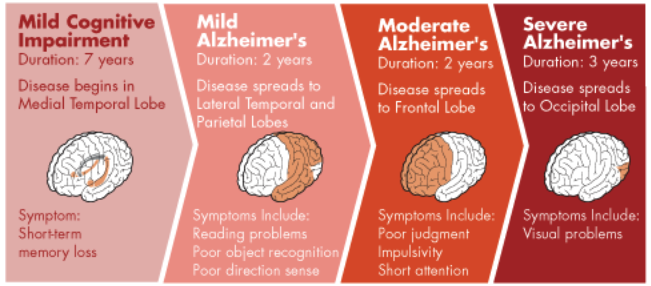
\includegraphics[width=5.20833in,height=\textheight]{img/ad_stages.png}

}

\caption{\label{fig-ad-progression}Alzheimer Disease Progression
(Credit: https://preventad.com/alzheimers-disease/)}

\end{figure}%

We estimate this order based on the biomarker data from patients'
visits. These data are typically results of neuropsych (e.g., MMSE)
and/or biological examiations (e.g., blood pressure). Visits data can be
longitudinal and/or cross-sectional, i.e., single visits from a cohort
of patients.

Knowing the disease progression is important because it helps prevent
and hopefully cure the disease. It also helps health professionals
prepare for the disease's further development.

We have several assumptions in EBM:

\begin{figure}

\centering{

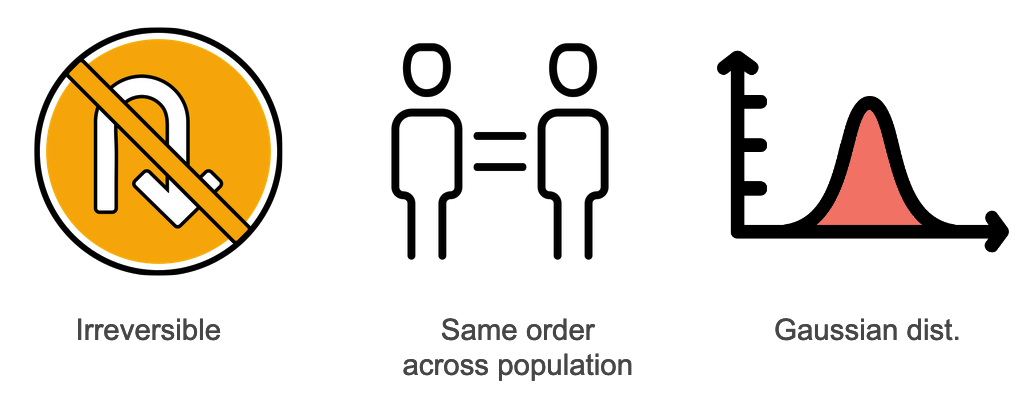
\includegraphics[width=5.20833in,height=\textheight]{img/assumptions.png}

}

\caption{\label{fig-ebm-assumptions}Assumptions of EBM}

\end{figure}%

\begin{itemize}
\tightlist
\item
  The disease is irreversible (i.e., a patient cannot go from stage 2 to
  stage 1)
\item
  The order in which different biomarkers get affected by the disease is
  the same across all patients.
\item
  Biomarker data can be approximated by a Gaussian distribution.
\end{itemize}

\begin{tcolorbox}[enhanced jigsaw, rightrule=.15mm, opacityback=0, leftrule=.75mm, colframe=quarto-callout-note-color-frame, colback=white, bottomrule=.15mm, toprule=.15mm, arc=.35mm, left=2mm, breakable]
\begin{minipage}[t]{5.5mm}
\textcolor{quarto-callout-note-color}{\faInfo}
\end{minipage}%
\begin{minipage}[t]{\textwidth - 5.5mm}

\vspace{-3mm}\textbf{Pay Attention}\vspace{3mm}

The third assumption, i.e., Gaussian approximation, isn't always hold.
However, for the purpose of our current method, we assume this is true.
There are other methods that do not assume Gaussian distributions, for
example, \href{https://github.com/ucl-pond/kde_ebm}{KDE EBM}, against
which we will compare results with later in our report.

\end{minipage}%
\end{tcolorbox}

This book contains chapters that explain step by step how we use the
event-based model to estimate the order of disease progression based on
cross-sectional patients' biomarker data.

\bookmarksetup{startatroot}

\chapter{EBM as A Generative Model}\label{sec-gen}

We can use EBM to generate synthetic biomarker data if we know:

\begin{itemize}
\tightlist
\item
  The order (\(S\)) in which different biomarkers get affected by the
  disease.
\item
  Parameters (i.e., mean and standard deviation) of biomarkers'
  distribution when they are affected (\(\theta\)) and not affected
  (\(\phi\)) by the disease.
\item
  Stages (\(k_j\)) that each participant is in.
\end{itemize}

Data we can generate looks like this:

\begin{figure}

\centering{

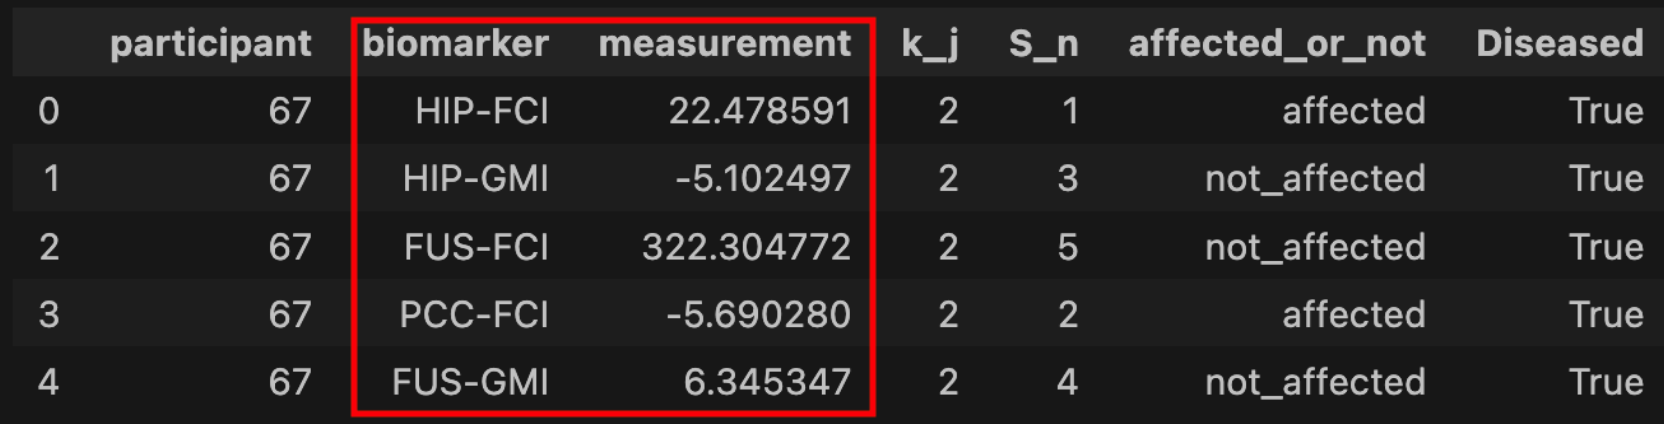
\includegraphics{img/sample_data.png}

}

\caption{\label{fig-sample-data}Sample Data}

\end{figure}%

This data is from a single participant.

As we mentioned above, to generate this data, we need to know:

\begin{itemize}
\tightlist
\item
  \(S\), i.e., the order of biomarkers. In the above example, \(S\) is
  HIP-FCI, PCC-FCI, HIP-GMI, FUS-GMI, FUS-FCI.
\item
  \(\mathcal N(\theta_{\mu}, \theta_{\sigma})\) and
  \(\mathcal N(\phi_{\mu}, \phi_{\sigma})\) for each of the five
  biomarkers, which are known but not shown directly here in the
  dataset.
\item
  \(k_j\), which is 2 in the above example.
\end{itemize}

We explain how this data is constructed in the following, column by
column.

First, the \texttt{participant} id is \(67\). The \texttt{biomarker}
indicates each of the five biomarkers examined and measured. The
\texttt{measurement} is the biomarkers' measurement. \texttt{k\_j} is
the participant's stage. If this stage is above 0, it means
\texttt{Diseased\ =\ True}. \texttt{S\_n} indicates the \(n\)-th rank in
the order. If \texttt{k\_j\ \textless{}\ S\_n}, it means the
participant's stage hasn't reached that biomarker's rank; therefore,
this biomarker is \texttt{not\ affected}. If
\texttt{k\_j\ \textgreater{}=\ S\_n}, then this biomarker is
\texttt{affected}.

If a biomarker is \texttt{affected}, then its measurement comes from
\(\mathcal N(\theta_{\mu}, \theta_{\sigma})\) of that biomarker; if
\texttt{not\_affected}, \(\mathcal N(\phi_{\mu}, \phi_{\sigma})\).

\section{Generative Process}\label{generative-process}

The generative process of biomarker measurements can be described as:

\begin{equation}\phantomsection\label{eq-gen}{
X_{nj} \mid S, k_j, \theta_n, \phi_n \sim I(z_j = 1) \bigg[ I(S(n) \leq k_j) \, p(X_{nj} \mid \theta_{n}) + I(S(n) > k_j) \, p(X_{nj} \mid \phi_{n}) \bigg] \\
+ \left(1 - I(z_j = 1) \right) p(X_{nj} \mid \phi_{n})
}\end{equation}

This model says that given that we know
\(S, k_j, \theta_n, \text{and } \phi_n\), we can draw the biomarker
measurement from a distribution.

\(S \sim \mathrm{UniformPermutation}(\cdot)\)

\(S\) follows a distribution of uniform permutation. That means the
ordering of biomarkers is random.

\(k_j \sim \mathrm{DiscreteUniform}(N)\)

\(k_j\) follows a discrete uniform distribution, which means a
participant is equally likely to fall in a progression stage (e.g., from
\(0\) to \(5\), where \(0\) indicate this participant is healthy.)

\section{Graphical Explanation}\label{graphical-explanation}

In the following, we explain the generative model in three different
scenarios using
\href{https://en.wikipedia.org/wiki/Graphical_model}{graphical models}:
(1) All participants are healthy; (2) Both healthy and diseased
participants, but all biomarkers are affected among diseased people; (3)
Both healthy and diseased participants, but we do not whether biomarkers
are affected or not among patients.

\subsection{Scenario 1}\label{scenario-1}

If all participants are healthy:

\begin{equation}\phantomsection\label{eq-gen-s1}{
X_{nj} \sim p(X_{nj} \mid \phi_{n})
}\end{equation}

Where

\(X_{nj}\) indicates the measurement of biomarker \(n\) in participant
\(j\).

\(\phi_{n}\) represents \(\mathcal N(\phi_{\mu}, \phi_{\sigma})\) for
biomarker \(n\).

The graphical model would look like:

\begin{figure}

\centering{

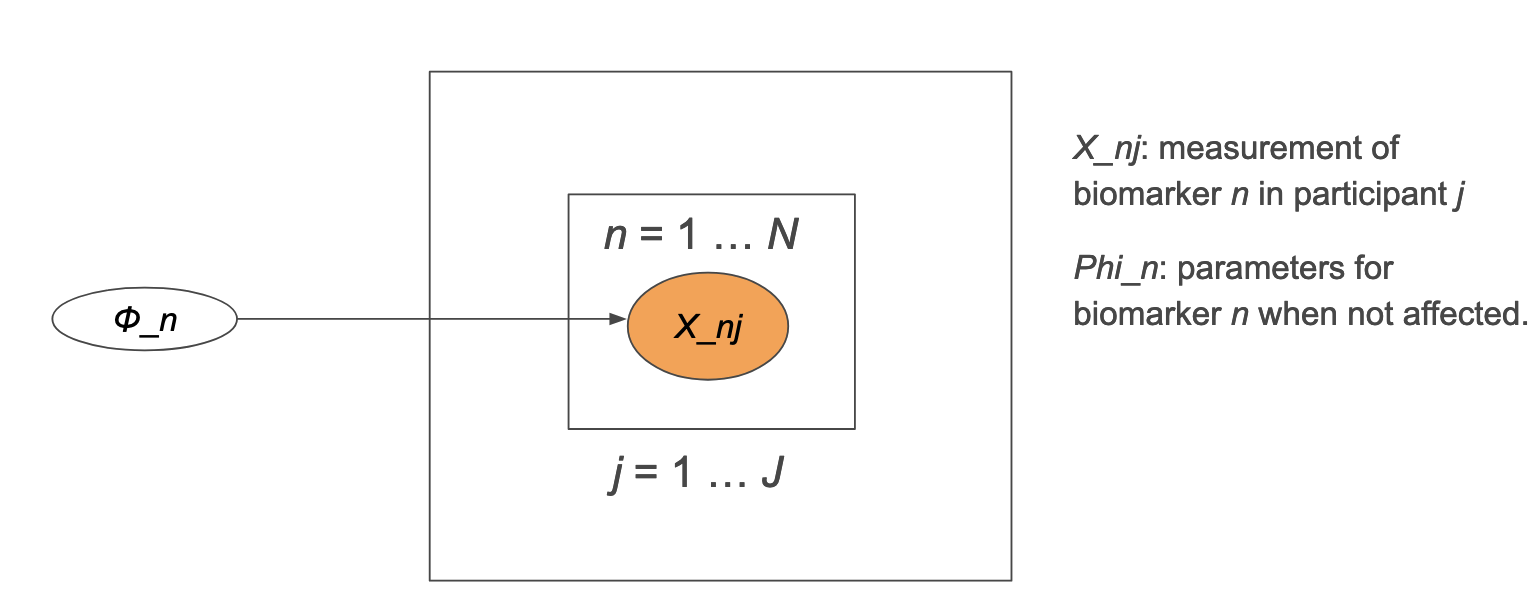
\includegraphics{img/g1.png}

}

\caption{\label{fig-g1}Graphical Model of Scenario 1}

\end{figure}%

\subsection{Scenario 2}\label{scenario-2}

If we have oth diseased and healthy participants, and all biomarkers are
affected among diseased participants.

\begin{equation}\phantomsection\label{eq-gen-s2}{
X_{nj} \sim I(z_j == 1) p(X_{nj} \mid \theta_n) + (1-I(z_j == 1))p(X_{nj} \mid \phi_n)
}\end{equation}

Where:

\(z_j = 1\) indicates this participant is diseased and \(z_j = 1\)
represents a healthy participant.

\(I(True) = 1\) and \(I(False) = 0\).

\(\theta_{n}\) represents \(\mathcal N(\theta_{\mu}, \theta_{\sigma})\)
for biomarker \(n\).

The graphical model would look like:

\begin{figure}

\centering{

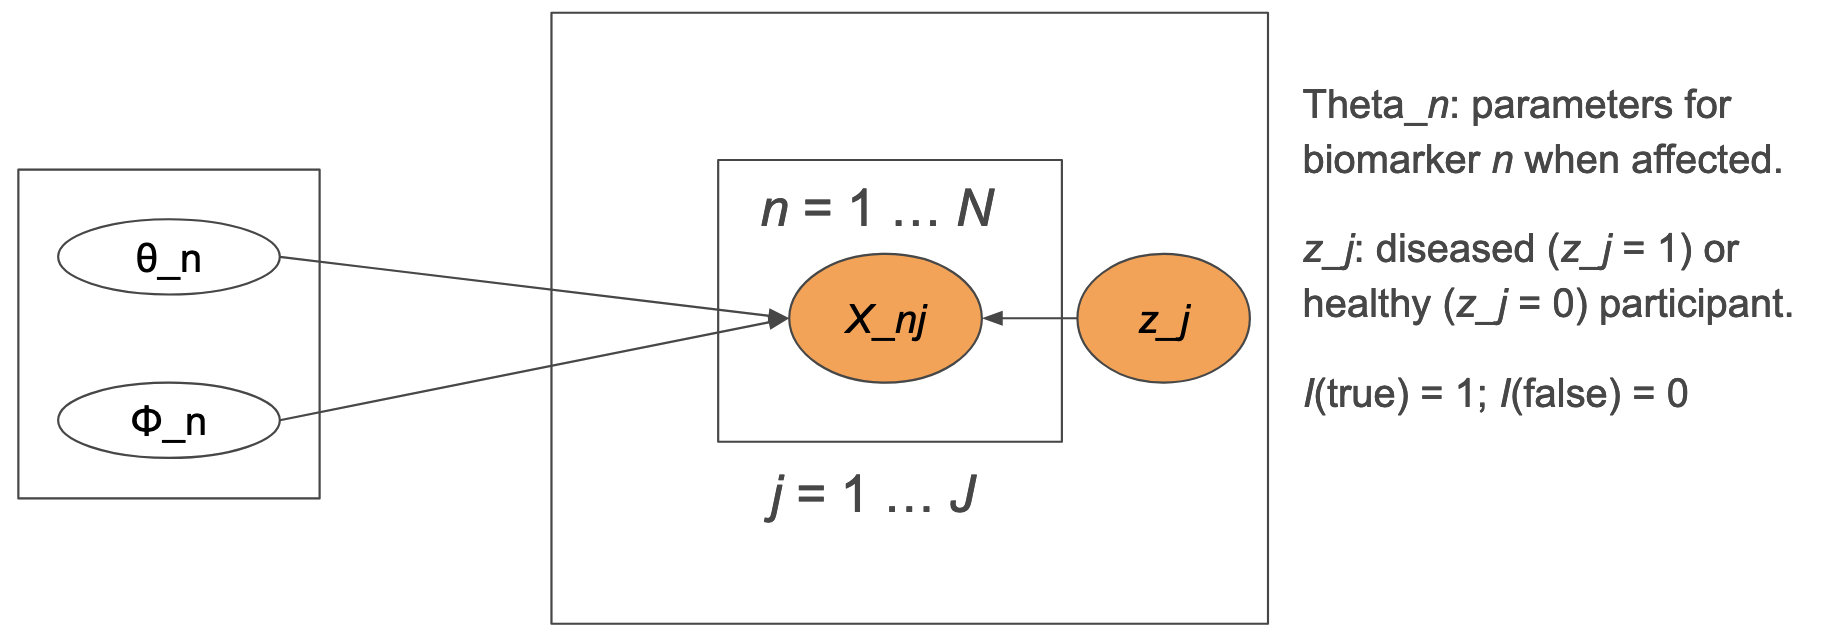
\includegraphics{img/g2.png}

}

\caption{\label{fig-g2}Graphical Model of Scenario 2}

\end{figure}%

\subsection{Scenario 3}\label{scenario-3}

If we have both healthy and diseased participants, but we do not whether
biomarkers are affected or not among patients, see
Equation~\ref{eq-gen}.

This is the model in usual cases.

The graphical model looks like:

\begin{figure}

\centering{

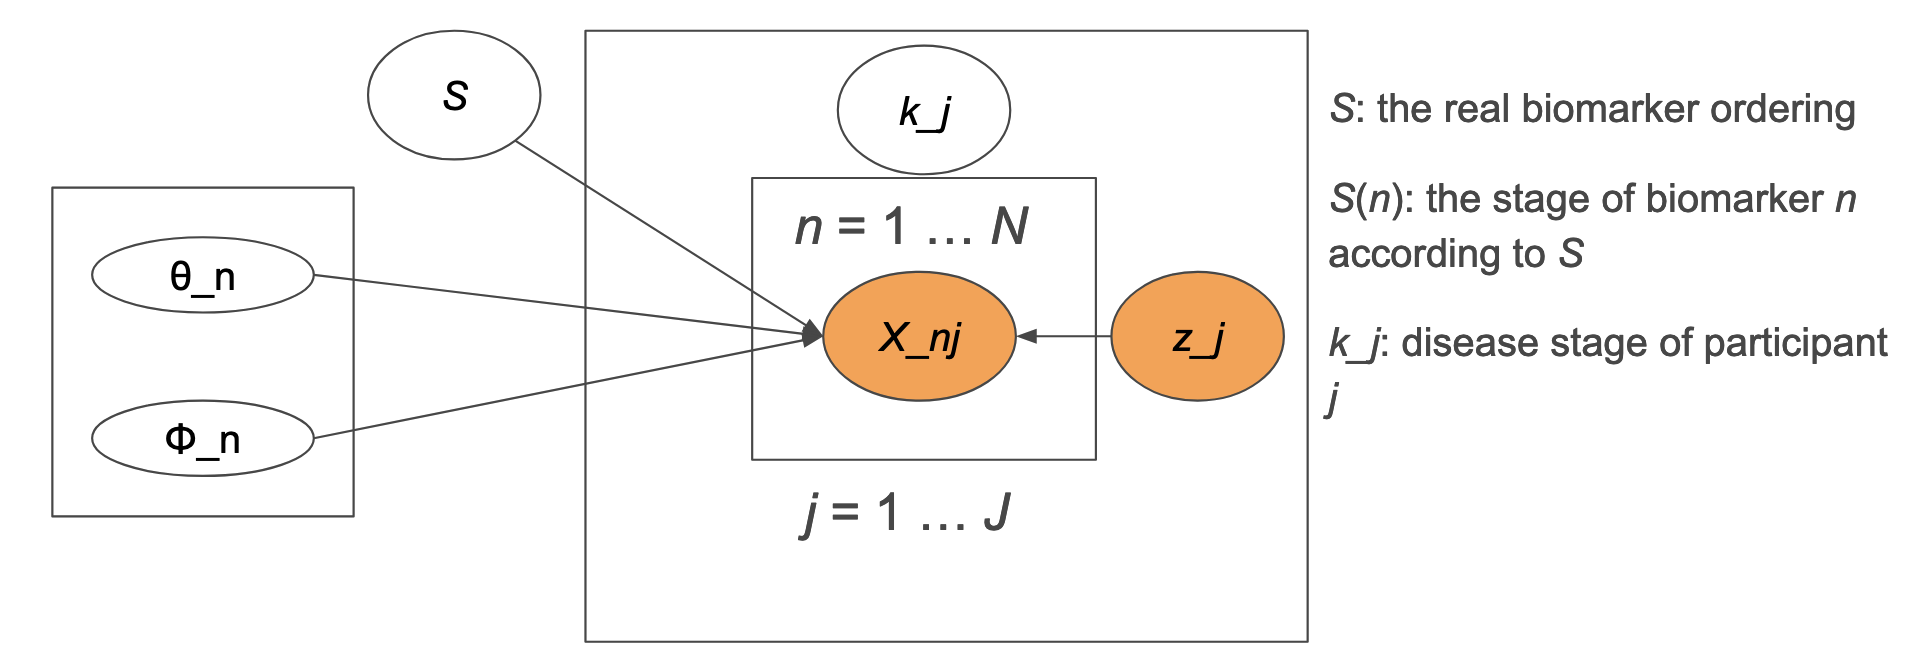
\includegraphics{img/g3.png}

}

\caption{\label{fig-g3}Graphical Model of Scenario 3}

\end{figure}%

\bookmarksetup{startatroot}

\chapter{Calculate the Likelihood of Biomarker
Measurements}\label{sec-calc-ll}

Suppose we have a participant's data, for example,
Figure~\ref{fig-sample-data}. Now, the question is:

\begin{quote}
What is the likelihood of this participant having this sequence of
biomarker data, given that we know \(S, \theta, \phi\).
\end{quote}

In the following, we explain how to calculate this likelihood in two
scenartios: (1) known \(k_j\) and (2) unknown \(k_j\).

\section{\texorpdfstring{Known \(k_j\)}{Known k\_j}}\label{known-k_j}

\begin{equation}\phantomsection\label{eq-known-kj}{
p(X_{j} | S, z_j = 1, k_j) = \underbrace{\prod_{i=1}^{k_j}{p(X_{S(i)j} \mid \theta_{S(i)} )}}_{\text{Affected biomarker likelihood}} \, 
\underbrace{\prod_{i=k_j+1}^N{p(X_{S(i)j} \mid \phi_{S(i)})}}_{\text{Non-affected biomarker likelihood}}
}\end{equation}

This equation compuates the likelihood of the observed biomarker data of
a specific participant, given that we know the disease stage this
patient is at (\(k_j\)).

\begin{itemize}
\item
  \(S\) is an \textbf{orded array} of biomarkers that are affected by
  the disease, for example, \([b, a, d, c]\). This means that biomarker
  \(b\) is affected at stage 1. At stage 2, biomarker \(b\) and \(a\)
  will be affected.
\item
  \(S(i)\) is the \(i^{th}\) biomarker according to \(S\). For example
  \(S_1\) will be biomarker \(b\).
\item
  \(k_j\) indicates the stage the patient is at, for example,
  \(k_j = 2\). This means that the disease has effected biomarker \(a\)
  and \(b\). Biomarker \(c\) and \(d\) have not been affected yet.
\item
  \(\theta_{S(i)}\) is the parameters for the probability density
  function (PDF) of observed value of biomarker \(S(i)\) when this
  biomarker has been affected by the disease. Let's assume this
  distribution is a Gaussian distribution with means of
  \([45, 50, 55, 60]\) and a standard deviation of \(5\) for biomarker
  \(b\), \(a\), \(d\), and \(c\).
\item
  \(\phi_{S(i)}\) is the parameters for the probability density function
  (PDF) of observed value of biomarker \(S(i)\) when this biomarker has
  \textbf{NOT} been affected by the disease. Let's assume this
  distribution is a Gaussian distribution with means of
  \([25, 30, 35, 40]\) and a standard deviation of \(3\) for biomarker
  \(b\), \(a\), \(d\), and \(c\).
\item
  \(X_j\) is an array representing the patient's observed data for all
  biomarker. Assume the data is \([77, 45, 53, 90]\) for biomarker
  \(b\), \(a\), \(d\), and \(c\).
\end{itemize}

We assume that the patient is at stage \(2\) of this disease; hence
\(k_j = 2\).

Next, we are going to calculate \(p(X_j|S, z_j = 1, k_j)\):

When \(i = 1\), we have \(S_{(i)} = b\) and \(X_{S_{(i)}} = X_b = 45\).
So

\[p(X_{S_{(i)}} | \theta_{S(i)}) = \frac{1}{\sigma \sqrt{2 \pi}} e^{-\frac{1}{2}\left(\frac{X_b - \mu}{\sigma} \right)^2}\]

Because \(k_j = 2\), so biomarker \(b\) and \(a\) are affected. We
should use the distribution of \(\theta_b\); therefore, we should plug
in \(\mu = 45, \sigma = 5\) in the above equation.

We can do the same for \(i\) = 2, 3, and 4.

So

\[p(X_j | S, k_j = 2) = p (X_b | \theta_b) \times p (X_a | \theta_a) \times p (X_d | \phi_d) \times p (X_c | \phi_c)\]

The above is the likelihood of the given biomarker data when
\(k_j = 2\).

Note that \(p (X_b | \theta_b)\) is probability density, a value of a
probability density function at a specific point; so it is not a
probability itself.

\textbf{Multiplying multiple probability densities will give us a
likelihood}.

\section{\texorpdfstring{Unknown
\(k_j\)}{Unknown k\_j}}\label{unknown-k_j}

\begin{equation}\phantomsection\label{eq-unknown-kj}{
P(X_{j} | S) = \sum_{k_j=0}^N{P(k_j) p(X_{j} \mid S, k_j)}
}\end{equation}

Suppose we have the same information above, except that we do not know
at which disease stage the patient is, i.e., we do not know \(k_j\). We
have the observed biomarker data: \(X_j = [77, 45, 53, 90]\). And I
wonder: what is the likelihood of seeing this specific ovserved data?

We assume that all five stages (including \(k_j = 0\)) are equally
likely.

We do not know \(k_j\), so the best option is to calculate the
``average'' likelihood of all the biomarker data.

Based on Equation~\ref{eq-known-kj}, we can calculate the following:

\(L_1 = p(X_j | S, k_j = 1)\)

\(L_2 = p(X_j | S, k_j = 2)\)

\(L_3 = p(X_j | S, k_j = 3)\)

\(L_4 = p(X_j | S, k_j = 4)\)

If this participant is healthy, then we know \(k_j = 0\), therefore:

\[L = L_0 = p(X_j | S, k_j = 0) = p (X_b | \phi_b) \times p (X_a | \phi_a) \times p (X_d | \phi_d) \times p (X_c | \phi_c)\]

If this participant is diseased but we do not know the actual \(k_j\),
we can estimate it this way

\[L_1 = p(X_j | S, k_j = 1) = p (X_b | \theta_b) \times p (X_a | \phi_a) \times p (X_d | \phi_d) \times p (X_c | \phi_c)\]

\[L_2 = p(X_j | S, k_j = 2) = p (X_b | \theta_b) \times p (X_a | \theta_a) \times p (X_d | \phi_d) \times p (X_c | \phi_c)\]

\[L_3 = p(X_j | S, k_j = 3) = p (X_b | \theta_b) \times p (X_a | \theta_a) \times p (X_d | \theta_d) \times p (X_c | \phi_c)\]

\[L_4 = p(X_j | S, k_j = 4) = p (X_b | \theta_b) \times p (X_a | \theta_a) \times p (X_d | \theta_d) \times p (X_c | \theta_c)\]

\(P(k_j)\) is the prior likelihood of being at stage \(k\).
\textbf{Event based models assume a uniform prior on \(k_j\)}.
Therefore:

\(P(X_{j} | z_j=1, S) = \frac{1}{4} \left(L_1 + L_2 + L_3 + L_4 \right)\)

\begin{tcolorbox}[enhanced jigsaw, bottomrule=.15mm, colback=white, bottomtitle=1mm, titlerule=0mm, arc=.35mm, breakable, rightrule=.15mm, opacityback=0, leftrule=.75mm, opacitybacktitle=0.6, colframe=quarto-callout-tip-color-frame, coltitle=black, toptitle=1mm, colbacktitle=quarto-callout-tip-color!10!white, title=\textcolor{quarto-callout-tip-color}{\faLightbulb}\hspace{0.5em}{Tip}, left=2mm, toprule=.15mm]

When this participant is diseased but we do not know the actual stage of
this participant, the above method is useful also because it hints at
the relative likelihood of each possible stage. For example, if L2 is
much larger than L1, L3, and L4, then we know this participant is most
likely to be at stage 2.

\end{tcolorbox}

\section{Extension}\label{extension}

If we are more interested in the likelihood of a whole dataset
consisting of all participants, we multiply all participants'
likelihood:
\(L = L_{P_1} \times L_{P_2} \times L_{P_3} ... \times L_{P_j}\).
Because this number tends to be very large, we take the natural log of
\(L\), i.e., \(\ln(L)\).

\bookmarksetup{startatroot}

\chapter{Generate Synthetic Data}\label{generate-synthetic-data}

In this chapter, we talk about how we generate the synthetic data of
participants' biomarker measurements. These data are used to test our
algorithms.

\section{Obtain Estimated Distribution
Parameters}\label{obtain-estimated-distribution-parameters}

In Chapter~\ref{sec-gen}, we mentioned that EBM can be used as a
generative model and we need to know \(S, \theta, \phi\) and \(k_j\).

First, we obtained \(S, \theta, \phi\) from Chen et al. (2016):

\begin{figure}

\centering{

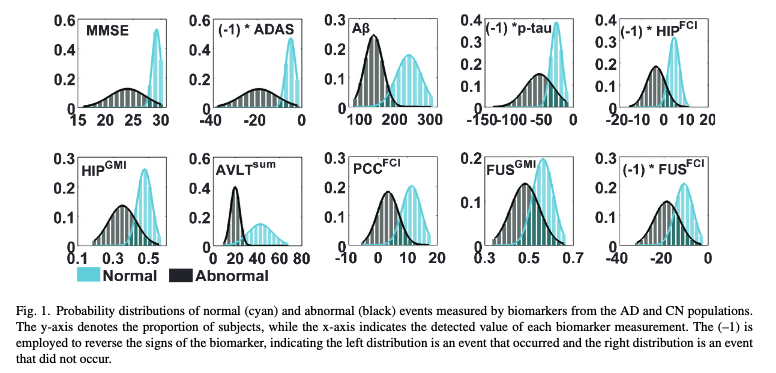
\includegraphics{img/chen1.png}

}

\caption{\label{fig-chen1}Theta and Phi from Chen's Paper}

\end{figure}%

\begin{figure}

\centering{

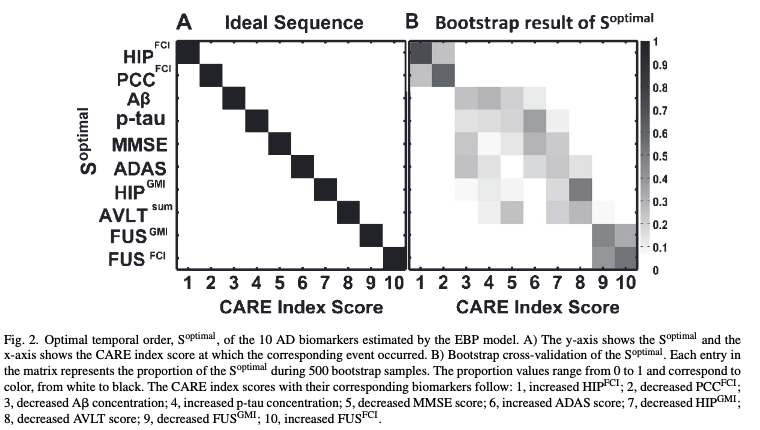
\includegraphics{img/chen2.png}

}

\caption{\label{fig-chen2}S from Chen's Paper}

\end{figure}%

This is our estimation:

\begin{Shaded}
\begin{Highlighting}[]
\ImportTok{import}\NormalTok{ pandas }\ImportTok{as}\NormalTok{ pd }
\ImportTok{import}\NormalTok{ numpy }\ImportTok{as}\NormalTok{ np }
\ImportTok{import}\NormalTok{ matplotlib.pyplot }\ImportTok{as}\NormalTok{ plt }
\ImportTok{import}\NormalTok{ json }
\ImportTok{import}\NormalTok{ scipy.stats }\ImportTok{as}\NormalTok{ stats}
\ImportTok{from}\NormalTok{ typing }\ImportTok{import}\NormalTok{ List, Optional, Tuple, Dict}
\ImportTok{import}\NormalTok{ os }
\ImportTok{import}\NormalTok{ seaborn }\ImportTok{as}\NormalTok{ sns}
\ImportTok{import}\NormalTok{ altair }\ImportTok{as}\NormalTok{ alt }
\end{Highlighting}
\end{Shaded}

\begin{Shaded}
\begin{Highlighting}[]
\NormalTok{all\_ten\_biomarker\_names }\OperatorTok{=}\NormalTok{ np.array([}
    \StringTok{\textquotesingle{}MMSE\textquotesingle{}}\NormalTok{, }\StringTok{\textquotesingle{}ADAS\textquotesingle{}}\NormalTok{, }\StringTok{\textquotesingle{}AB\textquotesingle{}}\NormalTok{, }\StringTok{\textquotesingle{}P{-}Tau\textquotesingle{}}\NormalTok{, }\StringTok{\textquotesingle{}HIP{-}FCI\textquotesingle{}}\NormalTok{, }
    \StringTok{\textquotesingle{}HIP{-}GMI\textquotesingle{}}\NormalTok{, }\StringTok{\textquotesingle{}AVLT{-}Sum\textquotesingle{}}\NormalTok{, }\StringTok{\textquotesingle{}PCC{-}FCI\textquotesingle{}}\NormalTok{, }\StringTok{\textquotesingle{}FUS{-}GMI\textquotesingle{}}\NormalTok{, }\StringTok{\textquotesingle{}FUS{-}FCI\textquotesingle{}}\NormalTok{])}
\CommentTok{\# in the order above}
\CommentTok{\# cyan, normal}
\NormalTok{phi\_means }\OperatorTok{=}\NormalTok{ [}\DecValTok{28}\NormalTok{, }\OperatorTok{{-}}\DecValTok{6}\NormalTok{, }\DecValTok{250}\NormalTok{, }\OperatorTok{{-}}\DecValTok{25}\NormalTok{, }\DecValTok{5}\NormalTok{, }\FloatTok{0.4}\NormalTok{, }\DecValTok{40}\NormalTok{, }\DecValTok{12}\NormalTok{, }\FloatTok{0.6}\NormalTok{, }\OperatorTok{{-}}\DecValTok{10}\NormalTok{]}
\CommentTok{\# black, abnormal}
\NormalTok{theta\_means }\OperatorTok{=}\NormalTok{ [}\DecValTok{22}\NormalTok{, }\OperatorTok{{-}}\DecValTok{20}\NormalTok{, }\DecValTok{150}\NormalTok{, }\OperatorTok{{-}}\DecValTok{50}\NormalTok{, }\OperatorTok{{-}}\DecValTok{5}\NormalTok{, }\FloatTok{0.3}\NormalTok{, }\DecValTok{20}\NormalTok{, }\DecValTok{5}\NormalTok{, }\FloatTok{0.5}\NormalTok{, }\OperatorTok{{-}}\DecValTok{20}\NormalTok{]}
\CommentTok{\# cyan, normal}
\NormalTok{phi\_std\_times\_three }\OperatorTok{=}\NormalTok{ [}\DecValTok{2}\NormalTok{, }\DecValTok{4}\NormalTok{, }\DecValTok{150}\NormalTok{, }\DecValTok{50}\NormalTok{, }\DecValTok{5}\NormalTok{, }\FloatTok{0.7}\NormalTok{, }\DecValTok{45}\NormalTok{, }\DecValTok{12}\NormalTok{, }\FloatTok{0.2}\NormalTok{, }\DecValTok{10}\NormalTok{]}
\NormalTok{phi\_stds }\OperatorTok{=}\NormalTok{ [std\_dev}\OperatorTok{/}\DecValTok{3} \ControlFlowTok{for}\NormalTok{ std\_dev }\KeywordTok{in}\NormalTok{ phi\_std\_times\_three]}
\CommentTok{\# black, abnormal}
\NormalTok{theta\_std\_times\_three }\OperatorTok{=}\NormalTok{ [}\DecValTok{8}\NormalTok{, }\DecValTok{12}\NormalTok{, }\DecValTok{50}\NormalTok{, }\DecValTok{100}\NormalTok{, }\DecValTok{20}\NormalTok{, }\DecValTok{1}\NormalTok{, }\DecValTok{20}\NormalTok{, }\DecValTok{10}\NormalTok{, }\FloatTok{0.2}\NormalTok{, }\DecValTok{18}\NormalTok{]}
\NormalTok{theta\_stds }\OperatorTok{=}\NormalTok{ [std\_dev}\OperatorTok{/}\DecValTok{3} \ControlFlowTok{for}\NormalTok{ std\_dev }\KeywordTok{in}\NormalTok{ theta\_std\_times\_three]}

\CommentTok{\# to get the real\_theta\_phi means and stds}
\NormalTok{hashmap\_of\_dicts }\OperatorTok{=}\NormalTok{ \{\}}
\ControlFlowTok{for}\NormalTok{ i, biomarker }\KeywordTok{in} \BuiltInTok{enumerate}\NormalTok{(all\_ten\_biomarker\_names):}
\NormalTok{    dic }\OperatorTok{=}\NormalTok{ \{\}}
    \CommentTok{\# dic = \{"biomarker": biomarker\}}
\NormalTok{    dic[}\StringTok{\textquotesingle{}theta\_mean\textquotesingle{}}\NormalTok{] }\OperatorTok{=}\NormalTok{ theta\_means[i]}
\NormalTok{    dic[}\StringTok{\textquotesingle{}theta\_std\textquotesingle{}}\NormalTok{] }\OperatorTok{=}\NormalTok{ theta\_stds[i]}
\NormalTok{    dic[}\StringTok{\textquotesingle{}phi\_mean\textquotesingle{}}\NormalTok{] }\OperatorTok{=}\NormalTok{ phi\_means[i]}
\NormalTok{    dic[}\StringTok{\textquotesingle{}phi\_std\textquotesingle{}}\NormalTok{] }\OperatorTok{=}\NormalTok{ phi\_stds[i]}
\NormalTok{    hashmap\_of\_dicts[biomarker] }\OperatorTok{=}\NormalTok{ dic }
\NormalTok{hashmap\_of\_dicts}

\NormalTok{real\_theta\_phi }\OperatorTok{=}\NormalTok{ pd.DataFrame(hashmap\_of\_dicts).transpose().reset\_index(names}\OperatorTok{=}\NormalTok{[}\StringTok{\textquotesingle{}biomarker\textquotesingle{}}\NormalTok{])}
\NormalTok{real\_theta\_phi}
\end{Highlighting}
\end{Shaded}

\begin{longtable}[]{@{}llllll@{}}
\toprule\noalign{}
& biomarker & theta\_mean & theta\_std & phi\_mean & phi\_std \\
\midrule\noalign{}
\endhead
\bottomrule\noalign{}
\endlastfoot
0 & MMSE & 22.0 & 2.666667 & 28.0 & 0.666667 \\
1 & ADAS & -20.0 & 4.000000 & -6.0 & 1.333333 \\
2 & AB & 150.0 & 16.666667 & 250.0 & 50.000000 \\
3 & P-Tau & -50.0 & 33.333333 & -25.0 & 16.666667 \\
4 & HIP-FCI & -5.0 & 6.666667 & 5.0 & 1.666667 \\
5 & HIP-GMI & 0.3 & 0.333333 & 0.4 & 0.233333 \\
6 & AVLT-Sum & 20.0 & 6.666667 & 40.0 & 15.000000 \\
7 & PCC-FCI & 5.0 & 3.333333 & 12.0 & 4.000000 \\
8 & FUS-GMI & 0.5 & 0.066667 & 0.6 & 0.066667 \\
9 & FUS-FCI & -20.0 & 6.000000 & -10.0 & 3.333333 \\
\end{longtable}

Store the parameters to a \texttt{JSON} file:

\begin{Shaded}
\begin{Highlighting}[]
\ControlFlowTok{with} \BuiltInTok{open}\NormalTok{(}\StringTok{\textquotesingle{}files/real\_theta\_phi.json\textquotesingle{}}\NormalTok{, }\StringTok{\textquotesingle{}w\textquotesingle{}}\NormalTok{) }\ImportTok{as}\NormalTok{ fp:}
\NormalTok{    json.dump(hashmap\_of\_dicts, fp)}
\end{Highlighting}
\end{Shaded}

\begin{Shaded}
\begin{Highlighting}[]
\NormalTok{biomarkers }\OperatorTok{=}\NormalTok{ all\_ten\_biomarker\_names}
\NormalTok{n\_biomarkers }\OperatorTok{=} \BuiltInTok{len}\NormalTok{(biomarkers)}

\KeywordTok{def}\NormalTok{ plot\_distribution\_pair(ax, mu1, sigma1, mu2, sigma2, title):}
    \CommentTok{"""mu1, sigma1: theta}
\CommentTok{    mu2, sigma2: phi}
\CommentTok{    """}
\NormalTok{    xmin }\OperatorTok{=} \BuiltInTok{min}\NormalTok{(mu1 }\OperatorTok{{-}} \DecValTok{4}\OperatorTok{*}\NormalTok{sigma1, mu2}\OperatorTok{{-}}\DecValTok{4}\OperatorTok{*}\NormalTok{sigma2)}
\NormalTok{    xmax }\OperatorTok{=} \BuiltInTok{max}\NormalTok{(mu1 }\OperatorTok{+} \DecValTok{4}\OperatorTok{*}\NormalTok{sigma1, mu2 }\OperatorTok{+} \DecValTok{4}\OperatorTok{*}\NormalTok{sigma2)}
\NormalTok{    x }\OperatorTok{=}\NormalTok{ np.linspace(xmin, xmax, }\DecValTok{1000}\NormalTok{)}
\NormalTok{    y1 }\OperatorTok{=}\NormalTok{ stats.norm.pdf(x, loc }\OperatorTok{=}\NormalTok{ mu1, scale }\OperatorTok{=}\NormalTok{ sigma1)}
\NormalTok{    y2 }\OperatorTok{=}\NormalTok{ stats.norm.pdf(x, loc }\OperatorTok{=}\NormalTok{ mu2, scale }\OperatorTok{=}\NormalTok{ sigma2)}
\NormalTok{    ax.plot(x, y1, label }\OperatorTok{=} \StringTok{"Abnormal"}\NormalTok{, color }\OperatorTok{=} \StringTok{"black"}\NormalTok{)}
\NormalTok{    ax.plot(x, y2, label }\OperatorTok{=} \StringTok{"Normal"}\NormalTok{, color }\OperatorTok{=} \StringTok{"cyan"}\NormalTok{)}
\NormalTok{    ax.fill\_between(x, y1, alpha }\OperatorTok{=} \FloatTok{0.3}\NormalTok{, color }\OperatorTok{=} \StringTok{"black"}\NormalTok{)}
\NormalTok{    ax.fill\_between(x, y2, alpha }\OperatorTok{=} \FloatTok{0.3}\NormalTok{, color }\OperatorTok{=} \StringTok{"cyan"}\NormalTok{)}
\NormalTok{    ax.set\_title(title)}
\NormalTok{    ax.legend()}

\NormalTok{fig, axes }\OperatorTok{=}\NormalTok{ plt.subplots(}\DecValTok{2}\NormalTok{, n\_biomarkers}\OperatorTok{//}\DecValTok{2}\NormalTok{, figsize}\OperatorTok{=}\NormalTok{(}\DecValTok{20}\NormalTok{, }\DecValTok{10}\NormalTok{))}
\ControlFlowTok{for}\NormalTok{ i, biomarker }\KeywordTok{in} \BuiltInTok{enumerate}\NormalTok{(biomarkers):}
\NormalTok{    ax }\OperatorTok{=}\NormalTok{ axes.flatten()[i] }
\NormalTok{    mu1, sigma1, mu2, sigma2 }\OperatorTok{=}\NormalTok{ real\_theta\_phi[}
\NormalTok{        real\_theta\_phi.biomarker }\OperatorTok{==}\NormalTok{ biomarker].reset\_index().iloc[}\DecValTok{0}\NormalTok{, :][}\DecValTok{2}\NormalTok{:].values}
\NormalTok{    plot\_distribution\_pair(}
\NormalTok{        ax, mu1, sigma1, mu2, sigma2, title }\OperatorTok{=}\NormalTok{ biomarker)}
\end{Highlighting}
\end{Shaded}

\begin{figure}[H]

\centering{

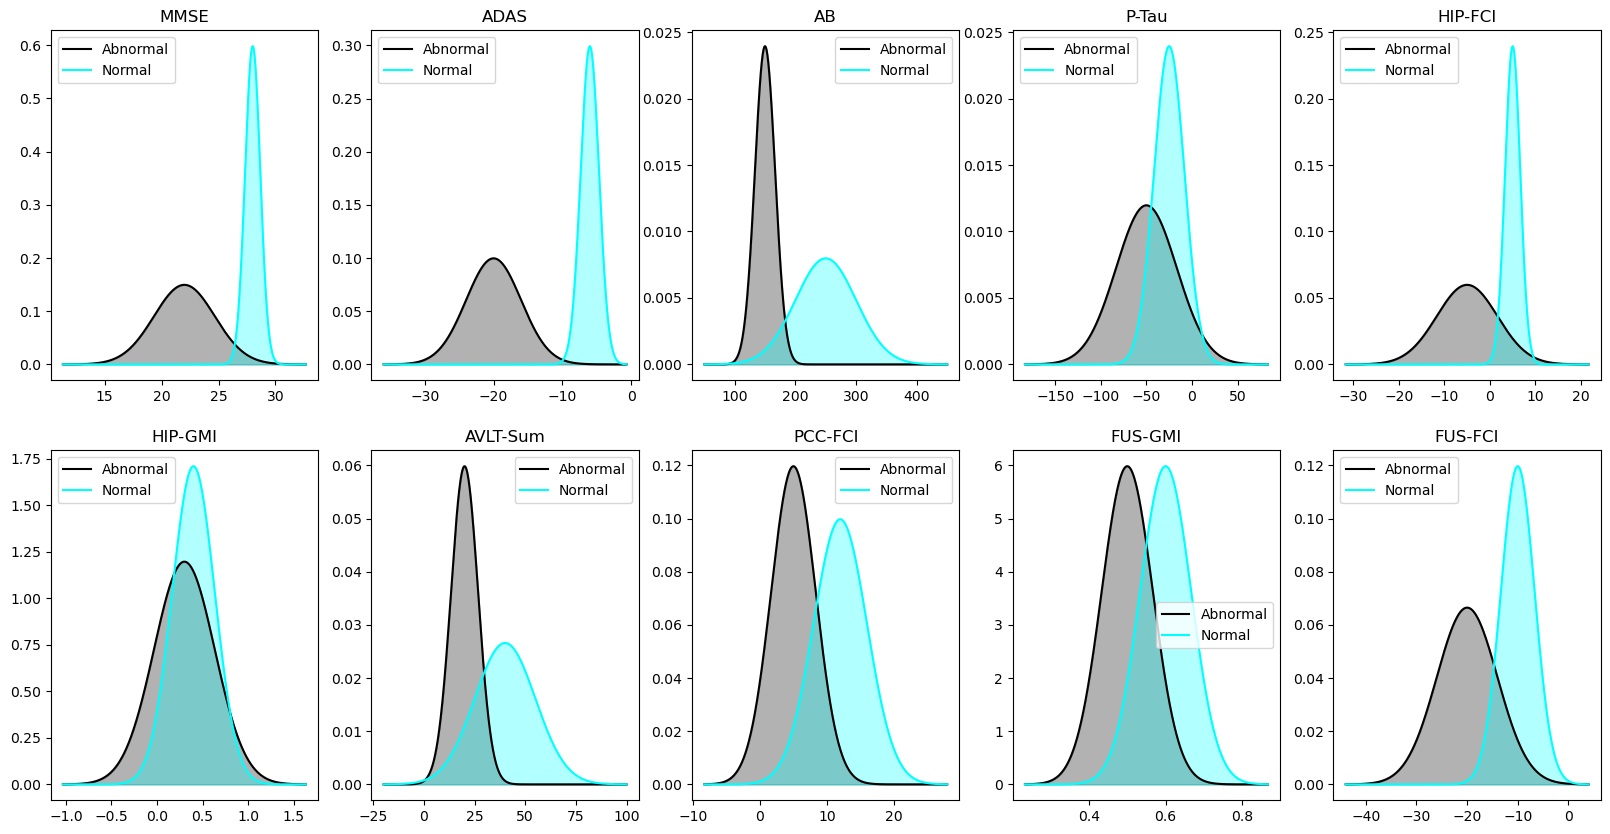
\includegraphics{gen_files/figure-pdf/fig-eval-theta-phi-estimations-output-1.png}

}

\caption{\label{fig-eval-theta-phi-estimations}evaluate theta and phi
estimations}

\end{figure}%

You can compare this to Figure~\ref{fig-chen1}.

\section{The Generating Process}\label{the-generating-process}

In the following, we explain our data generation process.

We have the following parameters:

\(J\): Number of participants.

\(R\): The percentage of healthy participants.

\(M\): Number of datasets per combination of \(j\) and \(r\).

We set these parameters:

\begin{Shaded}
\begin{Highlighting}[]
\NormalTok{js }\OperatorTok{=}\NormalTok{ [}\DecValTok{50}\NormalTok{, }\DecValTok{200}\NormalTok{, }\DecValTok{500}\NormalTok{]}
\NormalTok{rs }\OperatorTok{=}\NormalTok{ [}\FloatTok{0.1}\NormalTok{, }\FloatTok{0.25}\NormalTok{, }\FloatTok{0.5}\NormalTok{, }\FloatTok{0.75}\NormalTok{, }\FloatTok{0.9}\NormalTok{]}
\NormalTok{num\_of\_datasets\_per\_combination }\OperatorTok{=} \DecValTok{50}
\end{Highlighting}
\end{Shaded}

So, there will be \(3 \times 5 \times 50 = 750\) datasets to be
generated.

We define our \texttt{generate\_data\_from\_ebm} function:

\begin{Shaded}
\begin{Highlighting}[]
\KeywordTok{def}\NormalTok{ generate\_data\_from\_ebm(}
\NormalTok{    n\_participants: }\BuiltInTok{int}\NormalTok{,}
\NormalTok{    S\_ordering: List[}\BuiltInTok{str}\NormalTok{],}
\NormalTok{    real\_theta\_phi\_file: }\BuiltInTok{str}\NormalTok{,}
\NormalTok{    healthy\_ratio: }\BuiltInTok{float}\NormalTok{,}
\NormalTok{    output\_dir: }\BuiltInTok{str}\NormalTok{,}
\NormalTok{    m,  }\CommentTok{\# combstr\_m}
\NormalTok{    seed: Optional[}\BuiltInTok{int}\NormalTok{] }\OperatorTok{=} \DecValTok{0}
\NormalTok{) }\OperatorTok{{-}\textgreater{}}\NormalTok{ pd.DataFrame:}
    \CommentTok{"""}
\CommentTok{    Simulate an Event{-}Based Model (EBM) for disease progression.}

\CommentTok{    Args:}
\CommentTok{    n\_participants (int): Number of participants.}
\CommentTok{    S\_ordering (List[str]): Biomarker names ordered according to the order }
\CommentTok{        in which each of them get affected by the disease.}
\CommentTok{    real\_theta\_phi\_file (str): Directory of a JSON file which contains }
\CommentTok{        theta and phi values for all biomarkers.}
\CommentTok{        See real\_theta\_phi.json for example format.}
\CommentTok{    output\_dir (str): Directory where output files will be saved.}
\CommentTok{    healthy\_ratio (float): Proportion of healthy participants out of n\_participants.}
\CommentTok{    seed (Optional[int]): Seed for the random number generator for reproducibility.}

\CommentTok{    Returns:}
\CommentTok{    pd.DataFrame: A DataFrame with columns \textquotesingle{}participant\textquotesingle{}, "biomarker", \textquotesingle{}measurement\textquotesingle{}, }
\CommentTok{        \textquotesingle{}diseased\textquotesingle{}.}
\CommentTok{    """}
    \CommentTok{\# Parameter validation}
    \ControlFlowTok{assert}\NormalTok{ n\_participants }\OperatorTok{\textgreater{}} \DecValTok{0}\NormalTok{, }\StringTok{"Number of participants must be greater than 0."}
    \ControlFlowTok{assert} \DecValTok{0} \OperatorTok{\textless{}=}\NormalTok{ healthy\_ratio }\OperatorTok{\textless{}=} \DecValTok{1}\NormalTok{, }\StringTok{"Healthy ratio must be between 0 and 1."}

    \CommentTok{\# Set the seed for numpy\textquotesingle{}s random number generator}
\NormalTok{    rng }\OperatorTok{=}\NormalTok{ np.random.default\_rng(seed)}

    \CommentTok{\# Load theta and phi values from the JSON file}
    \ControlFlowTok{try}\NormalTok{:}
        \ControlFlowTok{with} \BuiltInTok{open}\NormalTok{(real\_theta\_phi\_file) }\ImportTok{as}\NormalTok{ f:}
\NormalTok{            real\_theta\_phi }\OperatorTok{=}\NormalTok{ json.load(f)}
    \ControlFlowTok{except} \PreprocessorTok{FileNotFoundError}\NormalTok{:}
        \ControlFlowTok{raise} \PreprocessorTok{FileNotFoundError}\NormalTok{(}\SpecialStringTok{f"File }\SpecialCharTok{\{}\NormalTok{real\_theta\_phi}\SpecialCharTok{\}}\SpecialStringTok{ not fount"}\NormalTok{)}
    \ControlFlowTok{except}\NormalTok{ json.JSONDecodeError:}
        \ControlFlowTok{raise} \PreprocessorTok{ValueError}\NormalTok{(}
            \SpecialStringTok{f"File }\SpecialCharTok{\{}\NormalTok{real\_theta\_phi\_file}\SpecialCharTok{\}}\SpecialStringTok{ is not a valid JSON file."}\NormalTok{)}

\NormalTok{    n\_biomarkers }\OperatorTok{=} \BuiltInTok{len}\NormalTok{(S\_ordering)}
\NormalTok{    n\_stages }\OperatorTok{=}\NormalTok{ n\_biomarkers }\OperatorTok{+} \DecValTok{1}

\NormalTok{    n\_healthy }\OperatorTok{=} \BuiltInTok{int}\NormalTok{(n\_participants }\OperatorTok{*}\NormalTok{ healthy\_ratio)}
\NormalTok{    n\_diseased }\OperatorTok{=} \BuiltInTok{int}\NormalTok{(n\_participants }\OperatorTok{{-}}\NormalTok{ n\_healthy)}

    \CommentTok{\# Generate disease stages}
\NormalTok{    kjs }\OperatorTok{=}\NormalTok{ np.concatenate((np.zeros(n\_healthy, dtype}\OperatorTok{=}\BuiltInTok{int}\NormalTok{),}
\NormalTok{                         rng.integers(}\DecValTok{1}\NormalTok{, n\_stages, n\_diseased)))}
    \CommentTok{\# shuffle so that it\textquotesingle{}s not 0s first and then disease stages bur all random}
\NormalTok{    rng.shuffle(kjs)}

    \CommentTok{\# Initiate biomarker measurement matrix (J participants x N biomarkers) with None}
\NormalTok{    X }\OperatorTok{=}\NormalTok{ np.full((n\_participants, n\_biomarkers), }\VariableTok{None}\NormalTok{, dtype}\OperatorTok{=}\BuiltInTok{object}\NormalTok{)}

    \CommentTok{\# Create distributions for each biomarker}
\NormalTok{    theta\_dist }\OperatorTok{=}\NormalTok{ \{biomarker: stats.norm(}
\NormalTok{        real\_theta\_phi[biomarker][}\StringTok{\textquotesingle{}theta\_mean\textquotesingle{}}\NormalTok{],}
\NormalTok{        real\_theta\_phi[biomarker][}\StringTok{\textquotesingle{}theta\_std\textquotesingle{}}\NormalTok{]}
\NormalTok{    ) }\ControlFlowTok{for}\NormalTok{ biomarker }\KeywordTok{in}\NormalTok{ S\_ordering\}}

\NormalTok{    phi\_dist }\OperatorTok{=}\NormalTok{ \{biomarker: stats.norm(}
\NormalTok{        real\_theta\_phi[biomarker][}\StringTok{\textquotesingle{}phi\_mean\textquotesingle{}}\NormalTok{],}
\NormalTok{        real\_theta\_phi[biomarker][}\StringTok{\textquotesingle{}phi\_std\textquotesingle{}}\NormalTok{]}
\NormalTok{    ) }\ControlFlowTok{for}\NormalTok{ biomarker }\KeywordTok{in}\NormalTok{ S\_ordering\}}

    \CommentTok{\# Populate the matrix with biomarker measurements}
    \ControlFlowTok{for}\NormalTok{ j }\KeywordTok{in} \BuiltInTok{range}\NormalTok{(n\_participants):}
        \ControlFlowTok{for}\NormalTok{ n, biomarker }\KeywordTok{in} \BuiltInTok{enumerate}\NormalTok{(S\_ordering):}
            \CommentTok{\# because for each j, we generate X[j, n] in the order of S\_ordering,}
            \CommentTok{\# the final dataset will have this ordering as well.}
\NormalTok{            k\_j }\OperatorTok{=}\NormalTok{ kjs[j]}
\NormalTok{            S\_n }\OperatorTok{=}\NormalTok{ n }\OperatorTok{+} \DecValTok{1}

            \CommentTok{\# Assign biomarker values based on the participant\textquotesingle{}s disease stage}
            \CommentTok{\# affected, or not\_affected, is regarding the biomarker, not the participant}
            \ControlFlowTok{if}\NormalTok{ k\_j }\OperatorTok{\textgreater{}=} \DecValTok{1}\NormalTok{:}
                \ControlFlowTok{if}\NormalTok{ k\_j }\OperatorTok{\textgreater{}=}\NormalTok{ S\_n:}
                    \CommentTok{\# rvs() is affected by np.random()}
\NormalTok{                    X[j, n] }\OperatorTok{=}\NormalTok{ (}
\NormalTok{                        j, biomarker, theta\_dist[biomarker].rvs(random\_state}\OperatorTok{=}\NormalTok{rng), k\_j, S\_n, }\StringTok{\textquotesingle{}affected\textquotesingle{}}\NormalTok{)}
                \ControlFlowTok{else}\NormalTok{:}
\NormalTok{                    X[j, n] }\OperatorTok{=}\NormalTok{ (j, biomarker, phi\_dist[biomarker].rvs(random\_state}\OperatorTok{=}\NormalTok{rng),}
\NormalTok{                               k\_j, S\_n, }\StringTok{\textquotesingle{}not\_affected\textquotesingle{}}\NormalTok{)}
            \CommentTok{\# if the participant is healthy}
            \ControlFlowTok{else}\NormalTok{:}
\NormalTok{                X[j, n] }\OperatorTok{=}\NormalTok{ (j, biomarker, phi\_dist[biomarker].rvs(random\_state}\OperatorTok{=}\NormalTok{rng),}
\NormalTok{                           k\_j, S\_n, }\StringTok{\textquotesingle{}not\_affected\textquotesingle{}}\NormalTok{)}

\NormalTok{    df }\OperatorTok{=}\NormalTok{ pd.DataFrame(X, columns}\OperatorTok{=}\NormalTok{S\_ordering)}
    \CommentTok{\# make this dataframe wide to long}
\NormalTok{    df\_long }\OperatorTok{=}\NormalTok{ df.melt(var\_name}\OperatorTok{=}\StringTok{"Biomarker"}\NormalTok{, value\_name}\OperatorTok{=}\StringTok{"Value"}\NormalTok{)}
\NormalTok{    data }\OperatorTok{=}\NormalTok{ df\_long[}\StringTok{\textquotesingle{}Value\textquotesingle{}}\NormalTok{].}\BuiltInTok{apply}\NormalTok{(pd.Series)}
\NormalTok{    data.columns }\OperatorTok{=}\NormalTok{ [}\StringTok{\textquotesingle{}participant\textquotesingle{}}\NormalTok{, }\StringTok{"biomarker"}\NormalTok{,}
                    \StringTok{\textquotesingle{}measurement\textquotesingle{}}\NormalTok{, }\StringTok{\textquotesingle{}k\_j\textquotesingle{}}\NormalTok{, }\StringTok{\textquotesingle{}S\_n\textquotesingle{}}\NormalTok{, }\StringTok{\textquotesingle{}affected\_or\_not\textquotesingle{}}\NormalTok{]}

    \CommentTok{\# biomarker\_name\_change\_dic = dict(}
    \CommentTok{\#     zip(S\_ordering, range(1, n\_biomarkers + 1)))}
\NormalTok{    data[}\StringTok{\textquotesingle{}diseased\textquotesingle{}}\NormalTok{] }\OperatorTok{=}\NormalTok{ data.}\BuiltInTok{apply}\NormalTok{(}\KeywordTok{lambda}\NormalTok{ row: row.k\_j }\OperatorTok{\textgreater{}} \DecValTok{0}\NormalTok{, axis}\OperatorTok{=}\DecValTok{1}\NormalTok{)}
    \CommentTok{\# data.drop([\textquotesingle{}k\_j\textquotesingle{}, \textquotesingle{}S\_n\textquotesingle{}, \textquotesingle{}affected\_or\_not\textquotesingle{}], axis=1, inplace=True)}
    \CommentTok{\# data[\textquotesingle{}biomarker\textquotesingle{}] = data.apply(}
    \CommentTok{\#     lambda row: f"\{row.biomarker\} (\{biomarker\_name\_change\_dic[row.biomarker]\})", axis=1)}

    \ControlFlowTok{if} \KeywordTok{not}\NormalTok{ os.path.exists(output\_dir):}
\NormalTok{        os.makedirs(output\_dir)}

\NormalTok{    filename }\OperatorTok{=} \SpecialStringTok{f"}\SpecialCharTok{\{}\BuiltInTok{int}\NormalTok{(healthy\_ratio}\OperatorTok{*}\NormalTok{n\_participants)}\SpecialCharTok{\}}\SpecialStringTok{|}\SpecialCharTok{\{}\NormalTok{n\_participants}\SpecialCharTok{\}}\SpecialStringTok{\_}\SpecialCharTok{\{}\NormalTok{m}\SpecialCharTok{\}}\SpecialStringTok{"}
\NormalTok{    data.to\_csv(}\SpecialStringTok{f\textquotesingle{}}\SpecialCharTok{\{}\NormalTok{output\_dir}\SpecialCharTok{\}}\SpecialStringTok{/}\SpecialCharTok{\{}\NormalTok{filename}\SpecialCharTok{\}}\SpecialStringTok{.csv\textquotesingle{}}\NormalTok{, index}\OperatorTok{=}\VariableTok{False}\NormalTok{)}
    \CommentTok{\# print("Data generation done! Output saved to:", filename)}
    \ControlFlowTok{return}\NormalTok{ data}
\end{Highlighting}
\end{Shaded}

\begin{Shaded}
\begin{Highlighting}[]
\NormalTok{S\_ordering }\OperatorTok{=}\NormalTok{ np.array([}
    \StringTok{\textquotesingle{}HIP{-}FCI\textquotesingle{}}\NormalTok{, }\StringTok{\textquotesingle{}PCC{-}FCI\textquotesingle{}}\NormalTok{, }\StringTok{\textquotesingle{}AB\textquotesingle{}}\NormalTok{, }\StringTok{\textquotesingle{}P{-}Tau\textquotesingle{}}\NormalTok{, }\StringTok{\textquotesingle{}MMSE\textquotesingle{}}\NormalTok{, }\StringTok{\textquotesingle{}ADAS\textquotesingle{}}\NormalTok{, }
    \StringTok{\textquotesingle{}HIP{-}GMI\textquotesingle{}}\NormalTok{, }\StringTok{\textquotesingle{}AVLT{-}Sum\textquotesingle{}}\NormalTok{, }\StringTok{\textquotesingle{}FUS{-}GMI\textquotesingle{}}\NormalTok{, }\StringTok{\textquotesingle{}FUS{-}FCI\textquotesingle{}}
\NormalTok{])}

\CommentTok{\# where the generated data will be saved}
\NormalTok{output\_dir }\OperatorTok{=} \StringTok{\textquotesingle{}data\textquotesingle{}}

\CommentTok{\# We run the following only once; once the data is generated, we no longer run it}
\CommentTok{\# We still show the codes to present our generation process}
\NormalTok{torun }\OperatorTok{=} \VariableTok{False}
\end{Highlighting}
\end{Shaded}

\begin{Shaded}
\begin{Highlighting}[]
\ControlFlowTok{if}\NormalTok{ torun:}
\NormalTok{    real\_theta\_phi\_file }\OperatorTok{=} \StringTok{\textquotesingle{}files/real\_theta\_phi.json\textquotesingle{}}
    \ControlFlowTok{for}\NormalTok{ j }\KeywordTok{in}\NormalTok{ js:}
        \ControlFlowTok{for}\NormalTok{ r }\KeywordTok{in}\NormalTok{ rs:}
            \ControlFlowTok{for}\NormalTok{ m }\KeywordTok{in} \BuiltInTok{range}\NormalTok{(}\DecValTok{0}\NormalTok{, num\_of\_datasets\_per\_combination):}
\NormalTok{                generate\_data\_from\_ebm(}
\NormalTok{                    n\_participants}\OperatorTok{=}\NormalTok{j,}
\NormalTok{                    S\_ordering}\OperatorTok{=}\NormalTok{S\_ordering,}
\NormalTok{                    real\_theta\_phi\_file}\OperatorTok{=}\NormalTok{real\_theta\_phi\_file,}
\NormalTok{                    healthy\_ratio}\OperatorTok{=}\NormalTok{r,}
\NormalTok{                    output\_dir}\OperatorTok{=}\NormalTok{output\_dir,}
\NormalTok{                    m}\OperatorTok{=}\NormalTok{m,}
\NormalTok{                    seed }\OperatorTok{=} \BuiltInTok{int}\NormalTok{(j}\OperatorTok{*}\DecValTok{10} \OperatorTok{+}\NormalTok{ (r }\OperatorTok{*} \DecValTok{100}\NormalTok{) }\OperatorTok{+}\NormalTok{ m),}
\NormalTok{                )}
        \BuiltInTok{print}\NormalTok{(}\SpecialStringTok{f\textquotesingle{}Done for J=}\SpecialCharTok{\{}\NormalTok{j}\SpecialCharTok{\}}\SpecialStringTok{\textquotesingle{}}\NormalTok{)}
\end{Highlighting}
\end{Shaded}

\section{Visualize Synthetic Data}\label{visualize-synthetic-data}

Above, we have generated 750 datasets, named in the fashion of
\texttt{150\textbar{}200\_3}, which means the third dataset when
\(j = 200\) and \(r = 0.75\).

Next, we try to visualize this dataset.

\begin{Shaded}
\begin{Highlighting}[]
\NormalTok{df }\OperatorTok{=}\NormalTok{ pd.read\_csv(}\SpecialStringTok{f"}\SpecialCharTok{\{}\NormalTok{output\_dir}\SpecialCharTok{\}}\SpecialStringTok{/150|200\_3.csv"}\NormalTok{)}
\NormalTok{df.head()}
\end{Highlighting}
\end{Shaded}

\begin{longtable}[]{@{}llllllll@{}}
\toprule\noalign{}
& participant & biomarker & measurement & k\_j & S\_n &
affected\_or\_not & diseased \\
\midrule\noalign{}
\endhead
\bottomrule\noalign{}
\endlastfoot
0 & 0 & HIP-FCI & 3.135981 & 0 & 1 & not\_affected & False \\
1 & 1 & HIP-FCI & 12.593704 & 2 & 1 & affected & True \\
2 & 2 & HIP-FCI & 6.220776 & 0 & 1 & not\_affected & False \\
3 & 3 & HIP-FCI & 3.545100 & 0 & 1 & not\_affected & False \\
4 & 4 & HIP-FCI & 3.966541 & 0 & 1 & not\_affected & False \\
\end{longtable}

\begin{Shaded}
\begin{Highlighting}[]
\NormalTok{df.shape}
\end{Highlighting}
\end{Shaded}

\begin{verbatim}
(2000, 7)
\end{verbatim}

This dataset has \(2000\) rows because we have \(200\) participants and
\(10\) biomarkers.

\subsection{Distribution of all biomarker
values}\label{distribution-of-all-biomarker-values}

\begin{Shaded}
\begin{Highlighting}[]
\NormalTok{alt.renderers.enable(}\StringTok{\textquotesingle{}png\textquotesingle{}}\NormalTok{)}
\NormalTok{alt.Chart(df).transform\_density(}
    \StringTok{\textquotesingle{}measurement\textquotesingle{}}\NormalTok{,}
\NormalTok{    as\_}\OperatorTok{=}\NormalTok{[}\StringTok{\textquotesingle{}measurement\textquotesingle{}}\NormalTok{, }\StringTok{\textquotesingle{}Density\textquotesingle{}}\NormalTok{],}
\NormalTok{    groupby}\OperatorTok{=}\NormalTok{[}\StringTok{\textquotesingle{}biomarker\textquotesingle{}}\NormalTok{]}
\NormalTok{).mark\_area().encode(}
\NormalTok{    x}\OperatorTok{=}\StringTok{"measurement:Q"}\NormalTok{,}
\NormalTok{    y}\OperatorTok{=}\StringTok{"Density:Q"}\NormalTok{,}
\NormalTok{    facet }\OperatorTok{=}\NormalTok{ alt.Facet(}
        \StringTok{"biomarker:N"}\NormalTok{,}
\NormalTok{        columns }\OperatorTok{=} \DecValTok{5}
\NormalTok{    ),}
\NormalTok{    color}\OperatorTok{=}\NormalTok{alt.Color(}
        \StringTok{\textquotesingle{}biomarker:N\textquotesingle{}}
\NormalTok{    )}
\NormalTok{).properties(}
\NormalTok{    width}\OperatorTok{=} \DecValTok{100}\NormalTok{,}
\NormalTok{    height }\OperatorTok{=} \DecValTok{180}\NormalTok{,}
\NormalTok{).properties(}
\NormalTok{    title}\OperatorTok{=}\StringTok{\textquotesingle{}Distribution of biomarker measurments\textquotesingle{}}
\NormalTok{)}
\end{Highlighting}
\end{Shaded}

\begin{figure}[H]

\centering{

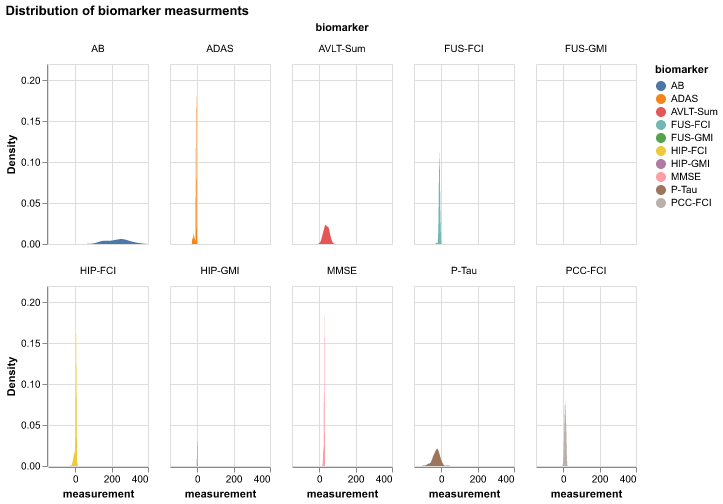
\includegraphics[width=7.53125in,height=5.25in]{gen_files/figure-pdf/fig-dist-biomarker-vals-output-1.png}

}

\caption{\label{fig-dist-biomarker-vals}Distribution of biomarker
measurments}

\end{figure}%

\subsection{Distribution of A Specific
Biomarker}\label{distribution-of-a-specific-biomarker}

\begin{Shaded}
\begin{Highlighting}[]
\NormalTok{idx }\OperatorTok{=} \DecValTok{1}
\NormalTok{biomarkers }\OperatorTok{=}\NormalTok{ df.biomarker.unique()}
\NormalTok{bio\_data }\OperatorTok{=}\NormalTok{ df[df.biomarker}\OperatorTok{==}\NormalTok{biomarkers[idx]]}
\NormalTok{alt.Chart(bio\_data).transform\_density(}
    \StringTok{\textquotesingle{}measurement\textquotesingle{}}\NormalTok{,}
\NormalTok{    as\_}\OperatorTok{=}\NormalTok{[}\StringTok{\textquotesingle{}measurement\textquotesingle{}}\NormalTok{, }\StringTok{\textquotesingle{}Density\textquotesingle{}}\NormalTok{],}
\NormalTok{    groupby}\OperatorTok{=}\NormalTok{[}\StringTok{\textquotesingle{}affected\_or\_not\textquotesingle{}}\NormalTok{]}
\NormalTok{).mark\_area().encode(}
\NormalTok{    x}\OperatorTok{=}\StringTok{"measurement:Q"}\NormalTok{,}
\NormalTok{    y}\OperatorTok{=}\StringTok{"Density:Q"}\NormalTok{,}
\NormalTok{    facet }\OperatorTok{=}\NormalTok{ alt.Facet(}
        \StringTok{"affected\_or\_not:N"}\NormalTok{,}
\NormalTok{    ),}
\NormalTok{    color}\OperatorTok{=}\NormalTok{alt.Color(}
        \StringTok{\textquotesingle{}affected\_or\_not:N\textquotesingle{}}
\NormalTok{    )}
\NormalTok{).properties(}
\NormalTok{    width}\OperatorTok{=} \DecValTok{240}\NormalTok{,}
\NormalTok{    height }\OperatorTok{=} \DecValTok{200}\NormalTok{,}
\NormalTok{).properties(}
\NormalTok{    title}\OperatorTok{=}\SpecialStringTok{f\textquotesingle{}Distribution of }\SpecialCharTok{\{}\NormalTok{biomarker}\SpecialCharTok{\}}\SpecialStringTok{ measurements\textquotesingle{}}
\NormalTok{)}
\end{Highlighting}
\end{Shaded}

\begin{figure}[H]

\centering{

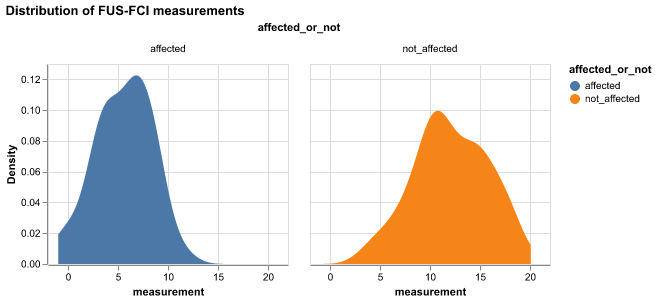
\includegraphics[width=6.84375in,height=3.14583in]{gen_files/figure-pdf/fig-dist-specific-biomarker-vals-output-1.png}

}

\caption{\label{fig-dist-specific-biomarker-vals}Distribution of HIP-FCI
measurements, compring bewteen affected and non-affected group}

\end{figure}%

\subsection{Looking into A Specific
Participant}\label{looking-into-a-specific-participant}

\begin{Shaded}
\begin{Highlighting}[]
\NormalTok{pidx }\OperatorTok{=} \DecValTok{1}
\NormalTok{p\_data }\OperatorTok{=}\NormalTok{ df[df.participant }\OperatorTok{==}\NormalTok{ pidx]}
\NormalTok{p\_data}
\end{Highlighting}
\end{Shaded}

\begin{longtable}[]{@{}llllllll@{}}
\toprule\noalign{}
& participant & biomarker & measurement & k\_j & S\_n &
affected\_or\_not & diseased \\
\midrule\noalign{}
\endhead
\bottomrule\noalign{}
\endlastfoot
1 & 1 & HIP-FCI & 12.593704 & 2 & 1 & affected & True \\
201 & 1 & PCC-FCI & 7.164017 & 2 & 2 & affected & True \\
401 & 1 & AB & 182.033823 & 2 & 3 & not\_affected & True \\
601 & 1 & P-Tau & -25.345325 & 2 & 4 & not\_affected & True \\
801 & 1 & MMSE & 27.600823 & 2 & 5 & not\_affected & True \\
1001 & 1 & ADAS & -4.920415 & 2 & 6 & not\_affected & True \\
1201 & 1 & HIP-GMI & 0.099052 & 2 & 7 & not\_affected & True \\
1401 & 1 & AVLT-Sum & 30.270797 & 2 & 8 & not\_affected & True \\
1601 & 1 & FUS-GMI & 0.658954 & 2 & 9 & not\_affected & True \\
1801 & 1 & FUS-FCI & -11.701559 & 2 & 10 & not\_affected & True \\
\end{longtable}

\begin{Shaded}
\begin{Highlighting}[]
\NormalTok{pidx }\OperatorTok{=}\DecValTok{1} \CommentTok{\# participant index}
\NormalTok{p\_data }\OperatorTok{=}\NormalTok{ df[df.participant }\OperatorTok{==}\NormalTok{ pidx]}
\NormalTok{alt.Chart(p\_data).mark\_bar().encode(}
\NormalTok{    x}\OperatorTok{=}\StringTok{\textquotesingle{}biomarker\textquotesingle{}}\NormalTok{,}
\NormalTok{    y}\OperatorTok{=}\StringTok{\textquotesingle{}measurement\textquotesingle{}}\NormalTok{,}
\NormalTok{    color}\OperatorTok{=}\NormalTok{alt.Color(}
        \StringTok{\textquotesingle{}affected\_or\_not:N\textquotesingle{}}
\NormalTok{    ),}
\NormalTok{    tooltip}\OperatorTok{=}\NormalTok{[}\StringTok{\textquotesingle{}biomarker\textquotesingle{}}\NormalTok{, }\StringTok{\textquotesingle{}affected\_or\_not\textquotesingle{}}\NormalTok{, }\StringTok{\textquotesingle{}measurement\textquotesingle{}}\NormalTok{]}
\NormalTok{).interactive().properties(}
\NormalTok{    title}\OperatorTok{=}\SpecialStringTok{f\textquotesingle{}Distribution of biomarker measurements for participant \#}\SpecialCharTok{\{}\NormalTok{idx}\SpecialCharTok{\}}\SpecialStringTok{ (k\_j = }\SpecialCharTok{\{}\NormalTok{p\_data}\SpecialCharTok{.}\NormalTok{k\_j}\SpecialCharTok{.}\NormalTok{to\_list()[}\DecValTok{0}\NormalTok{]}\SpecialCharTok{\}}\SpecialStringTok{)\textquotesingle{}}
\NormalTok{)}
\end{Highlighting}
\end{Shaded}

\begin{figure}[H]

\centering{

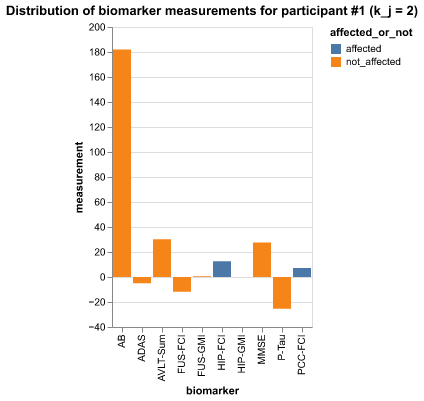
\includegraphics[width=4.41667in,height=4.17708in]{gen_files/figure-pdf/fig-dist-biomarker-vals-for-participant-output-1.png}

}

\caption{\label{fig-dist-biomarker-vals-for-participant}Distribution of
biomarker measurements for a specific participant}

\end{figure}%

\bookmarksetup{startatroot}

\chapter{Estimate Distribution
Parameters}\label{sec-estimate-dist-params}

Given \(S\), and a biomarker's measurements, how can we estimate
\(\mathcal N(\theta_{\mu}, \theta_{\sigma})\) and
\(\mathcal N(\phi_{\mu}, \phi_{\sigma})\)?

\begin{Shaded}
\begin{Highlighting}[]
\ImportTok{import}\NormalTok{ pandas }\ImportTok{as}\NormalTok{ pd}
\ImportTok{import}\NormalTok{ numpy }\ImportTok{as}\NormalTok{ np}
\ImportTok{import}\NormalTok{ matplotlib.pyplot }\ImportTok{as}\NormalTok{ plt }
\ImportTok{import}\NormalTok{ altair }\ImportTok{as}\NormalTok{ alt }
\ImportTok{import}\NormalTok{ math }
\ImportTok{from}\NormalTok{ scipy.stats }\ImportTok{import}\NormalTok{ norm}
\ImportTok{from}\NormalTok{ copkmeans.cop\_kmeans }\ImportTok{import}\NormalTok{ cop\_kmeans}
\ImportTok{from}\NormalTok{ typing }\ImportTok{import}\NormalTok{ Dict}
\ImportTok{import}\NormalTok{ re }
\ImportTok{import}\NormalTok{ json }
\ImportTok{from}\NormalTok{ collections }\ImportTok{import}\NormalTok{ defaultdict}
\end{Highlighting}
\end{Shaded}

\begin{Shaded}
\begin{Highlighting}[]
\NormalTok{output\_dir }\OperatorTok{=} \StringTok{\textquotesingle{}data\textquotesingle{}}
\NormalTok{df }\OperatorTok{=}\NormalTok{ pd.read\_csv(}\SpecialStringTok{f"}\SpecialCharTok{\{}\NormalTok{output\_dir}\SpecialCharTok{\}}\SpecialStringTok{/150|200\_3.csv"}\NormalTok{)}
\NormalTok{biomarkers }\OperatorTok{=}\NormalTok{ df.biomarker.unique()}
\NormalTok{idx }\OperatorTok{=} \DecValTok{1}
\NormalTok{biomarker\_df }\OperatorTok{=}\NormalTok{ df[df.biomarker}\OperatorTok{==}\NormalTok{biomarkers[idx]]}
\NormalTok{biomarker\_df.sample(}\DecValTok{10}\NormalTok{)}
\end{Highlighting}
\end{Shaded}

\begin{longtable}[]{@{}llllllll@{}}
\toprule\noalign{}
& participant & biomarker & measurement & k\_j & S\_n &
affected\_or\_not & diseased \\
\midrule\noalign{}
\endhead
\bottomrule\noalign{}
\endlastfoot
230 & 30 & PCC-FCI & 17.183986 & 0 & 2 & not\_affected & False \\
353 & 153 & PCC-FCI & 2.348147 & 6 & 2 & affected & True \\
397 & 197 & PCC-FCI & 10.062496 & 0 & 2 & not\_affected & False \\
232 & 32 & PCC-FCI & 12.526359 & 0 & 2 & not\_affected & False \\
316 & 116 & PCC-FCI & 15.028866 & 0 & 2 & not\_affected & False \\
305 & 105 & PCC-FCI & 3.762252 & 7 & 2 & affected & True \\
260 & 60 & PCC-FCI & 12.884854 & 0 & 2 & not\_affected & False \\
277 & 77 & PCC-FCI & 9.669905 & 0 & 2 & not\_affected & False \\
367 & 167 & PCC-FCI & 3.031575 & 5 & 2 & affected & True \\
208 & 8 & PCC-FCI & 10.352851 & 0 & 2 & not\_affected & False \\
\end{longtable}

\begin{Shaded}
\begin{Highlighting}[]
\NormalTok{biomarker\_df.shape}
\end{Highlighting}
\end{Shaded}

\begin{verbatim}
(200, 7)
\end{verbatim}

\section{Constrained K-Means}\label{sec-cop-kmeans}

\begin{tcolorbox}[enhanced jigsaw, bottomrule=.15mm, colback=white, bottomtitle=1mm, titlerule=0mm, arc=.35mm, breakable, rightrule=.15mm, opacityback=0, leftrule=.75mm, opacitybacktitle=0.6, colframe=quarto-callout-tip-color-frame, coltitle=black, toptitle=1mm, colbacktitle=quarto-callout-tip-color!10!white, title=\textcolor{quarto-callout-tip-color}{\faLightbulb}\hspace{0.5em}{Tip}, left=2mm, toprule=.15mm]

To use this algorithm, we only need to know (1) whether this participant
is diseased; and (2) each biomarker measurement.

\end{tcolorbox}

The first method we can use is constrained K-means, implemented by
Babaki (2017).

We choose constrained K-Means instead of the standard K-Means algorithm
because we know all healthy participants have to belong to the same
cluster. The constrained K-Means algorithm can satisfy this constraint.

\begin{Shaded}
\begin{Highlighting}[]
\KeywordTok{def}\NormalTok{ compute\_theta\_phi\_for\_biomarker(biomarker\_df, max\_attempt }\OperatorTok{=} \DecValTok{100}\NormalTok{):}
    \CommentTok{"""get theta and phi parameters for this biomarker using constrained k{-}means}
\CommentTok{    input: }
\CommentTok{        {-} biomarker\_df: a pd.dataframe of a specific biomarker}
\CommentTok{    output: }
\CommentTok{        {-} a tuple: theta\_mean, theta\_std, phi\_mean, phi\_std}
\CommentTok{    """}
\NormalTok{    n\_clusters }\OperatorTok{=} \DecValTok{2}
\NormalTok{    measurements }\OperatorTok{=}\NormalTok{ np.array(biomarker\_df[}\StringTok{\textquotesingle{}measurement\textquotesingle{}}\NormalTok{]).reshape(}\OperatorTok{{-}}\DecValTok{1}\NormalTok{, }\DecValTok{1}\NormalTok{)}
\NormalTok{    healthy\_df }\OperatorTok{=}\NormalTok{ biomarker\_df[biomarker\_df[}\StringTok{\textquotesingle{}diseased\textquotesingle{}}\NormalTok{] }\OperatorTok{==} \VariableTok{False}\NormalTok{]}
\NormalTok{    must\_link }\OperatorTok{=}\NormalTok{ [(x, }\DecValTok{0}\NormalTok{) }\ControlFlowTok{for}\NormalTok{ x }\KeywordTok{in}\NormalTok{ healthy\_df.index]}
    \CommentTok{\# Implement Constrained K{-}means algorithm}
    \CommentTok{\# https://github.com/Behrouz{-}Babaki/COP{-}Kmeans}

\NormalTok{    curr\_attempt }\OperatorTok{=} \DecValTok{0}
    \ControlFlowTok{while}\NormalTok{ curr\_attempt }\OperatorTok{\textless{}}\NormalTok{ max\_attempt:}
\NormalTok{        clusters, centers }\OperatorTok{=}\NormalTok{ cop\_kmeans(}
\NormalTok{            dataset}\OperatorTok{=}\NormalTok{measurements, k}\OperatorTok{=}\NormalTok{n\_clusters, ml}\OperatorTok{=}\NormalTok{must\_link)}
\NormalTok{        predictions }\OperatorTok{=}\NormalTok{ np.array(clusters)}
\NormalTok{        healthy\_predictions }\OperatorTok{=}\NormalTok{ predictions[healthy\_df.index]}
\NormalTok{        cluster\_counts }\OperatorTok{=}\NormalTok{ np.bincount(predictions)}
        \ControlFlowTok{if} \BuiltInTok{all}\NormalTok{(}
\NormalTok{            c }\OperatorTok{\textgreater{}} \DecValTok{1} \ControlFlowTok{for}\NormalTok{ c }\KeywordTok{in}\NormalTok{ cluster\_counts) }\KeywordTok{and} \BuiltInTok{len}\NormalTok{(}
\NormalTok{                cluster\_counts) }\OperatorTok{==}\NormalTok{ n\_clusters }\KeywordTok{and} \BuiltInTok{len}\NormalTok{(}
                    \BuiltInTok{set}\NormalTok{(healthy\_predictions)) }\OperatorTok{==} \DecValTok{1}\NormalTok{:}
            \ControlFlowTok{break} 
\NormalTok{        curr\_attempt }\OperatorTok{+=} \DecValTok{1}
    
    \ControlFlowTok{if}\NormalTok{ curr\_attempt }\OperatorTok{\textgreater{}} \DecValTok{2}\NormalTok{:}
        \BuiltInTok{print}\NormalTok{(curr\_attempt)}

    \CommentTok{\# double check the result}
    \ControlFlowTok{if} \KeywordTok{not} \BuiltInTok{all}\NormalTok{(c }\OperatorTok{\textgreater{}} \DecValTok{1} \ControlFlowTok{for}\NormalTok{ c }\KeywordTok{in}\NormalTok{ cluster\_counts):}
        \ControlFlowTok{raise} \PreprocessorTok{ValueError}\NormalTok{(}\SpecialStringTok{f"Not all clusters have more than one node."}\NormalTok{)}
    \ControlFlowTok{if} \BuiltInTok{len}\NormalTok{(cluster\_counts) }\OperatorTok{!=}\NormalTok{ n\_clusters:}
        \ControlFlowTok{raise} \PreprocessorTok{ValueError}\NormalTok{(}\SpecialStringTok{f"Number of clusters is not equal to }\SpecialCharTok{\{}\NormalTok{n\_clusters}\SpecialCharTok{\}}\SpecialStringTok{."}\NormalTok{)}
    \ControlFlowTok{if} \BuiltInTok{len}\NormalTok{(}\BuiltInTok{set}\NormalTok{(healthy\_predictions)) }\OperatorTok{\textgreater{}} \DecValTok{1}\NormalTok{:}
        \ControlFlowTok{raise} \PreprocessorTok{ValueError}\NormalTok{(}\StringTok{"Not all healthy participants belong to one cluster."}\NormalTok{)}
    
\NormalTok{    phi\_cluster\_idx }\OperatorTok{=}\NormalTok{ healthy\_predictions[}\DecValTok{0}\NormalTok{]}
\NormalTok{    theta\_cluster\_idx }\OperatorTok{=} \DecValTok{1} \OperatorTok{{-}}\NormalTok{ phi\_cluster\_idx}

    \CommentTok{\# two empty clusters to strore measurements}
\NormalTok{    clustered\_measurements }\OperatorTok{=}\NormalTok{ [[] }\ControlFlowTok{for}\NormalTok{ \_ }\KeywordTok{in} \BuiltInTok{range}\NormalTok{(}\DecValTok{2}\NormalTok{)]}
    \CommentTok{\# Store measurements into their cluster}
    \ControlFlowTok{for}\NormalTok{ i, prediction }\KeywordTok{in} \BuiltInTok{enumerate}\NormalTok{(predictions):}
\NormalTok{        clustered\_measurements[prediction].append(measurements[i][}\DecValTok{0}\NormalTok{])}
    
     \CommentTok{\# Calculate means and standard deviations}
\NormalTok{    theta\_mean, theta\_std }\OperatorTok{=}\NormalTok{ np.mean(}
\NormalTok{        clustered\_measurements[theta\_cluster\_idx]), np.std(}
\NormalTok{            clustered\_measurements[theta\_cluster\_idx])}
\NormalTok{    phi\_mean, phi\_std }\OperatorTok{=}\NormalTok{ np.mean(}
\NormalTok{        clustered\_measurements[phi\_cluster\_idx]), np.std(}
\NormalTok{            clustered\_measurements[phi\_cluster\_idx])}
    
    \CommentTok{\# check whether the prior\_theta\_phi contain 0s or nan}
    \ControlFlowTok{if}\NormalTok{ math.isnan(theta\_std) }\KeywordTok{or}\NormalTok{ theta\_std }\OperatorTok{==} \DecValTok{0}\NormalTok{:}
        \ControlFlowTok{raise} \PreprocessorTok{ValueError}\NormalTok{(}\SpecialStringTok{f"Invalid theta\_std: }\SpecialCharTok{\{}\NormalTok{theta\_std}\SpecialCharTok{\}}\SpecialStringTok{"}\NormalTok{)}
    \ControlFlowTok{if}\NormalTok{ math.isnan(phi\_std) }\KeywordTok{or}\NormalTok{ phi\_std }\OperatorTok{==} \DecValTok{0}\NormalTok{:}
        \ControlFlowTok{raise} \PreprocessorTok{ValueError}\NormalTok{(}\SpecialStringTok{f"Invalid phi\_std: }\SpecialCharTok{\{}\NormalTok{phi\_std}\SpecialCharTok{\}}\SpecialStringTok{"}\NormalTok{)}
    \ControlFlowTok{if}\NormalTok{ theta\_mean }\OperatorTok{==} \DecValTok{0} \KeywordTok{or}\NormalTok{ math.isnan(theta\_mean):}
        \ControlFlowTok{raise} \PreprocessorTok{ValueError}\NormalTok{(}\SpecialStringTok{f"Invalid theta\_mean: }\SpecialCharTok{\{}\NormalTok{theta\_mean}\SpecialCharTok{\}}\SpecialStringTok{"}\NormalTok{)}
    \ControlFlowTok{if}\NormalTok{ phi\_mean }\OperatorTok{==} \DecValTok{0} \KeywordTok{or}\NormalTok{ math.isnan(phi\_mean):}
        \ControlFlowTok{raise} \PreprocessorTok{ValueError}\NormalTok{(}\SpecialStringTok{f"Invalid phi\_mean: }\SpecialCharTok{\{}\NormalTok{phi\_mean}\SpecialCharTok{\}}\SpecialStringTok{"}\NormalTok{)}

    \ControlFlowTok{return}\NormalTok{ theta\_mean, theta\_std, phi\_mean, phi\_std}

\KeywordTok{def}\NormalTok{ get\_theta\_phi\_estimates(}
\NormalTok{    data: pd.DataFrame,}
\NormalTok{) }\OperatorTok{{-}\textgreater{}}\NormalTok{ Dict[}\BuiltInTok{str}\NormalTok{, Dict[}\BuiltInTok{str}\NormalTok{, }\BuiltInTok{float}\NormalTok{]]:}
    \CommentTok{"""}
\CommentTok{    Obtain theta and phi estimates (mean and standard deviation) for each biomarker.}

\CommentTok{    Args:}
\CommentTok{    data (pd.DataFrame): DataFrame containing participant data with columns \textquotesingle{}participant\textquotesingle{}, }
\CommentTok{        \textquotesingle{}biomarker\textquotesingle{}, \textquotesingle{}measurement\textquotesingle{}, and \textquotesingle{}diseased\textquotesingle{}.}
\CommentTok{    \# biomarkers (List[str]): A list of biomarker names.}

\CommentTok{    Returns:}
\CommentTok{    Dict[str, Dict[str, float]]: A dictionary where each key is a biomarker name,}
\CommentTok{        and each value is another dictionary containing the means and standard deviations }
\CommentTok{        for theta and phi of that biomarker, with keys \textquotesingle{}theta\_mean\textquotesingle{}, \textquotesingle{}theta\_std\textquotesingle{}, \textquotesingle{}phi\_mean\textquotesingle{}, }
\CommentTok{        and \textquotesingle{}phi\_std\textquotesingle{}.}
\CommentTok{    """}
    \CommentTok{\# empty hashmap of dictionaries to store the estimates}
\NormalTok{    estimates }\OperatorTok{=}\NormalTok{ \{\}}
\NormalTok{    biomarkers }\OperatorTok{=}\NormalTok{ data.biomarker.unique()}
    \ControlFlowTok{for}\NormalTok{ biomarker }\KeywordTok{in}\NormalTok{ biomarkers:}
        \CommentTok{\# Filter data for the current biomarker}
        \CommentTok{\# reset\_index is necessary here because we will use healthy\_df.index later}
\NormalTok{        biomarker\_df }\OperatorTok{=}\NormalTok{ data[data[}\StringTok{\textquotesingle{}biomarker\textquotesingle{}}\NormalTok{]}
                            \OperatorTok{==}\NormalTok{ biomarker].reset\_index(drop}\OperatorTok{=}\VariableTok{True}\NormalTok{)}
\NormalTok{        theta\_mean, theta\_std, phi\_mean, phi\_std }\OperatorTok{=}\NormalTok{ compute\_theta\_phi\_for\_biomarker(}
\NormalTok{            biomarker\_df)}
\NormalTok{        estimates[biomarker] }\OperatorTok{=}\NormalTok{ \{}
            \StringTok{\textquotesingle{}theta\_mean\textquotesingle{}}\NormalTok{: theta\_mean,}
            \StringTok{\textquotesingle{}theta\_std\textquotesingle{}}\NormalTok{: theta\_std,}
            \StringTok{\textquotesingle{}phi\_mean\textquotesingle{}}\NormalTok{: phi\_mean,}
            \StringTok{\textquotesingle{}phi\_std\textquotesingle{}}\NormalTok{: phi\_std}
\NormalTok{        \}}
    \ControlFlowTok{return}\NormalTok{ estimates}
\end{Highlighting}
\end{Shaded}

\begin{Shaded}
\begin{Highlighting}[]
\NormalTok{cop\_kmeans\_estimates }\OperatorTok{=}\NormalTok{ get\_theta\_phi\_estimates(data }\OperatorTok{=}\NormalTok{ df)}
\NormalTok{cop\_kmeans\_estimates\_df }\OperatorTok{=}\NormalTok{ pd.DataFrame.from\_dict(}
\NormalTok{    cop\_kmeans\_estimates, orient}\OperatorTok{=}\StringTok{\textquotesingle{}index\textquotesingle{}}\NormalTok{)}
\NormalTok{cop\_kmeans\_estimates\_df.reset\_index(names }\OperatorTok{=} \StringTok{\textquotesingle{}biomarker\textquotesingle{}}\NormalTok{, inplace}\OperatorTok{=}\VariableTok{True}\NormalTok{)}
\NormalTok{cop\_kmeans\_estimates\_df}
\end{Highlighting}
\end{Shaded}

\begin{longtable}[]{@{}llllll@{}}
\toprule\noalign{}
& biomarker & theta\_mean & theta\_std & phi\_mean & phi\_std \\
\midrule\noalign{}
\endhead
\bottomrule\noalign{}
\endlastfoot
0 & HIP-FCI & -8.587833 & 5.365053 & 4.903437 & 2.008974 \\
1 & PCC-FCI & 16.330398 & 0.720160 & 10.507041 & 4.427907 \\
2 & AB & 152.194375 & 15.344414 & 252.969562 & 50.946400 \\
3 & P-Tau & -71.767059 & 15.231429 & -23.737466 & 16.637657 \\
4 & MMSE & 22.164115 & 1.555676 & 27.994652 & 0.832845 \\
5 & ADAS & -20.582091 & 3.853234 & -6.002048 & 1.487443 \\
6 & HIP-GMI & 0.114735 & 0.106857 & 0.404924 & 0.235082 \\
7 & AVLT-Sum & 60.569081 & 6.389012 & 38.169767 & 14.373474 \\
8 & FUS-GMI & 0.478209 & 0.041763 & 0.596322 & 0.059436 \\
9 & FUS-FCI & -19.200644 & 4.688806 & -9.568412 & 3.003514 \\
\end{longtable}

\begin{Shaded}
\begin{Highlighting}[]
\ControlFlowTok{with} \BuiltInTok{open}\NormalTok{(}\StringTok{\textquotesingle{}files/real\_theta\_phi.json\textquotesingle{}}\NormalTok{, }\StringTok{\textquotesingle{}r\textquotesingle{}}\NormalTok{) }\ImportTok{as}\NormalTok{ f:}
\NormalTok{    truth }\OperatorTok{=}\NormalTok{ json.load(f)}
\NormalTok{truth\_df }\OperatorTok{=}\NormalTok{ pd.DataFrame.from\_dict(truth, orient}\OperatorTok{=}\StringTok{\textquotesingle{}index\textquotesingle{}}\NormalTok{)}
\NormalTok{truth\_df.reset\_index(names }\OperatorTok{=} \StringTok{\textquotesingle{}biomarker\textquotesingle{}}\NormalTok{, inplace}\OperatorTok{=}\VariableTok{True}\NormalTok{)}
\NormalTok{truth\_df}
\end{Highlighting}
\end{Shaded}

\begin{longtable}[]{@{}llllll@{}}
\toprule\noalign{}
& biomarker & theta\_mean & theta\_std & phi\_mean & phi\_std \\
\midrule\noalign{}
\endhead
\bottomrule\noalign{}
\endlastfoot
0 & MMSE & 22.0 & 2.666667 & 28.0 & 0.666667 \\
1 & ADAS & -20.0 & 4.000000 & -6.0 & 1.333333 \\
2 & AB & 150.0 & 16.666667 & 250.0 & 50.000000 \\
3 & P-Tau & -50.0 & 33.333333 & -25.0 & 16.666667 \\
4 & HIP-FCI & -5.0 & 6.666667 & 5.0 & 1.666667 \\
5 & HIP-GMI & 0.3 & 0.333333 & 0.4 & 0.233333 \\
6 & AVLT-Sum & 20.0 & 6.666667 & 40.0 & 15.000000 \\
7 & PCC-FCI & 5.0 & 3.333333 & 12.0 & 4.000000 \\
8 & FUS-GMI & 0.5 & 0.066667 & 0.6 & 0.066667 \\
9 & FUS-FCI & -20.0 & 6.000000 & -10.0 & 3.333333 \\
\end{longtable}

Now let's compare the results using plots:

\begin{Shaded}
\begin{Highlighting}[]
\KeywordTok{def}\NormalTok{ obtain\_theta\_phi\_params(biomarker, estimate\_df, truth):}
    \CommentTok{\textquotesingle{}\textquotesingle{}\textquotesingle{}This is to obtain both true and estimated theta and phi params for each biomarker \textquotesingle{}\textquotesingle{}\textquotesingle{}}
\NormalTok{    biomarker\_data\_est }\OperatorTok{=}\NormalTok{ estimate\_df[estimate\_df.biomarker }\OperatorTok{==}\NormalTok{ biomarker].reset\_index()}
\NormalTok{    biomarker\_data }\OperatorTok{=}\NormalTok{ truth[truth.biomarker }\OperatorTok{==}\NormalTok{ biomarker].reset\_index()}
    \CommentTok{\# theta for affected}
\NormalTok{    theta\_mean\_est }\OperatorTok{=}\NormalTok{ biomarker\_data\_est.theta\_mean[}\DecValTok{0}\NormalTok{]}
\NormalTok{    theta\_std\_est }\OperatorTok{=}\NormalTok{ biomarker\_data\_est.theta\_std[}\DecValTok{0}\NormalTok{]}

\NormalTok{    theta\_mean }\OperatorTok{=}\NormalTok{ biomarker\_data.theta\_mean[}\DecValTok{0}\NormalTok{]}
\NormalTok{    theta\_std }\OperatorTok{=}\NormalTok{ biomarker\_data.theta\_std[}\DecValTok{0}\NormalTok{]}

    \CommentTok{\# phi for not affected}
\NormalTok{    phi\_mean\_est }\OperatorTok{=}\NormalTok{ biomarker\_data\_est.phi\_mean[}\DecValTok{0}\NormalTok{]}
\NormalTok{    phi\_std\_est }\OperatorTok{=}\NormalTok{ biomarker\_data\_est.phi\_std[}\DecValTok{0}\NormalTok{]}

\NormalTok{    phi\_mean }\OperatorTok{=}\NormalTok{ biomarker\_data.phi\_mean[}\DecValTok{0}\NormalTok{]}
\NormalTok{    phi\_std }\OperatorTok{=}\NormalTok{ biomarker\_data.phi\_std[}\DecValTok{0}\NormalTok{]}

    \ControlFlowTok{return}\NormalTok{ theta\_mean, theta\_std, theta\_mean\_est, theta\_std\_est, phi\_mean, phi\_std, phi\_mean\_est, phi\_std\_est}

\KeywordTok{def}\NormalTok{ make\_chart(biomarkers, estimate\_df, truth, title):}
\NormalTok{    alt.renderers.enable(}\StringTok{\textquotesingle{}png\textquotesingle{}}\NormalTok{)}
\NormalTok{    charts }\OperatorTok{=}\NormalTok{ []}
    \ControlFlowTok{for}\NormalTok{ biomarker }\KeywordTok{in}\NormalTok{ biomarkers: }
\NormalTok{        theta\_mean, theta\_std, theta\_mean\_est, theta\_std\_est, phi\_mean, phi\_std, phi\_mean\_est, phi\_std\_est }\OperatorTok{=}\NormalTok{ obtain\_theta\_phi\_params(}
\NormalTok{        biomarker, estimate\_df, truth)}
\NormalTok{        mean1, std1 }\OperatorTok{=}\NormalTok{ theta\_mean, theta\_std}
\NormalTok{        mean2, std2 }\OperatorTok{=}\NormalTok{ theta\_mean\_est, theta\_std\_est}

        \CommentTok{\# Generating points on the x axis}
\NormalTok{        x\_thetas }\OperatorTok{=}\NormalTok{ np.linspace(}\BuiltInTok{min}\NormalTok{(mean1 }\OperatorTok{{-}} \DecValTok{3}\OperatorTok{*}\NormalTok{std1, mean2 }\OperatorTok{{-}} \DecValTok{3}\OperatorTok{*}\NormalTok{std2), }
                        \BuiltInTok{max}\NormalTok{(mean1 }\OperatorTok{+} \DecValTok{3}\OperatorTok{*}\NormalTok{std1, mean2 }\OperatorTok{+} \DecValTok{3}\OperatorTok{*}\NormalTok{std2), }\DecValTok{1000}\NormalTok{)}

        \CommentTok{\# Creating DataFrames for each distribution}
\NormalTok{        df1 }\OperatorTok{=}\NormalTok{ pd.DataFrame(\{}\StringTok{\textquotesingle{}x\textquotesingle{}}\NormalTok{: x\_thetas, }\StringTok{\textquotesingle{}pdf\textquotesingle{}}\NormalTok{: norm.pdf(x\_thetas, mean1, std1), }\StringTok{\textquotesingle{}Distribution\textquotesingle{}}\NormalTok{: }\StringTok{\textquotesingle{}Actual\textquotesingle{}}\NormalTok{\})}
\NormalTok{        df2 }\OperatorTok{=}\NormalTok{ pd.DataFrame(\{}\StringTok{\textquotesingle{}x\textquotesingle{}}\NormalTok{: x\_thetas, }\StringTok{\textquotesingle{}pdf\textquotesingle{}}\NormalTok{: norm.pdf(x\_thetas, mean2, std2), }\StringTok{\textquotesingle{}Distribution\textquotesingle{}}\NormalTok{: }\StringTok{\textquotesingle{}Estimated\textquotesingle{}}\NormalTok{\})}

        \CommentTok{\# Combining the DataFrames}
\NormalTok{        df3 }\OperatorTok{=}\NormalTok{ pd.concat([df1, df2])}

        \CommentTok{\# Altair plot}
\NormalTok{        chart\_theta }\OperatorTok{=}\NormalTok{ alt.Chart(df3).mark\_line().encode(}
\NormalTok{            x}\OperatorTok{=}\StringTok{\textquotesingle{}x\textquotesingle{}}\NormalTok{,}
\NormalTok{            y}\OperatorTok{=}\StringTok{\textquotesingle{}pdf\textquotesingle{}}\NormalTok{,}
\NormalTok{            color}\OperatorTok{=}\NormalTok{alt.Color(}\StringTok{\textquotesingle{}Distribution:N\textquotesingle{}}\NormalTok{, legend}\OperatorTok{=}\NormalTok{alt.Legend(title}\OperatorTok{=}\StringTok{"Theta"}\NormalTok{))}
\NormalTok{        ).properties(}
\NormalTok{            title}\OperatorTok{=}\SpecialStringTok{f\textquotesingle{}}\SpecialCharTok{\{}\NormalTok{biomarker}\SpecialCharTok{\}}\SpecialStringTok{, Theta\textquotesingle{}}\NormalTok{,}
\NormalTok{            width}\OperatorTok{=}\DecValTok{100}\NormalTok{,}
\NormalTok{            height}\OperatorTok{=}\DecValTok{100}
\NormalTok{            )}

\NormalTok{        mean1, std1 }\OperatorTok{=}\NormalTok{ phi\_mean, phi\_std}
\NormalTok{        mean2, std2 }\OperatorTok{=}\NormalTok{ phi\_mean\_est, phi\_std\_est}

        \CommentTok{\# Generating points on the x axis}
\NormalTok{        x\_phis }\OperatorTok{=}\NormalTok{ np.linspace(}\BuiltInTok{min}\NormalTok{(mean1 }\OperatorTok{{-}} \DecValTok{3}\OperatorTok{*}\NormalTok{std1, mean2 }\OperatorTok{{-}} \DecValTok{3}\OperatorTok{*}\NormalTok{std2), }
                        \BuiltInTok{max}\NormalTok{(mean1 }\OperatorTok{+} \DecValTok{3}\OperatorTok{*}\NormalTok{std1, mean2 }\OperatorTok{+} \DecValTok{3}\OperatorTok{*}\NormalTok{std2), }\DecValTok{1000}\NormalTok{)}

        \CommentTok{\# Creating DataFrames for each distribution}
\NormalTok{        df1 }\OperatorTok{=}\NormalTok{ pd.DataFrame(\{}\StringTok{\textquotesingle{}x\textquotesingle{}}\NormalTok{: x\_phis, }\StringTok{\textquotesingle{}pdf\textquotesingle{}}\NormalTok{: norm.pdf(x\_phis, mean1, std1), }\StringTok{\textquotesingle{}Distribution\textquotesingle{}}\NormalTok{: }\StringTok{\textquotesingle{}Actual\textquotesingle{}}\NormalTok{\})}
\NormalTok{        df2 }\OperatorTok{=}\NormalTok{ pd.DataFrame(\{}\StringTok{\textquotesingle{}x\textquotesingle{}}\NormalTok{: x\_phis, }\StringTok{\textquotesingle{}pdf\textquotesingle{}}\NormalTok{: norm.pdf(x\_phis, mean2, std2), }\StringTok{\textquotesingle{}Distribution\textquotesingle{}}\NormalTok{: }\StringTok{\textquotesingle{}Estimated\textquotesingle{}}\NormalTok{\})}

        \CommentTok{\# Combining the DataFrames}
\NormalTok{        df3 }\OperatorTok{=}\NormalTok{ pd.concat([df1, df2])}

        \CommentTok{\# Altair plot}
\NormalTok{        chart\_phi }\OperatorTok{=}\NormalTok{ alt.Chart(df3).mark\_line().encode(}
\NormalTok{            x}\OperatorTok{=}\StringTok{\textquotesingle{}x\textquotesingle{}}\NormalTok{,}
\NormalTok{            y}\OperatorTok{=}\StringTok{\textquotesingle{}pdf\textquotesingle{}}\NormalTok{,}
\NormalTok{            color}\OperatorTok{=}\NormalTok{alt.Color(}\StringTok{\textquotesingle{}Distribution:N\textquotesingle{}}\NormalTok{, legend}\OperatorTok{=}\NormalTok{alt.Legend(title}\OperatorTok{=}\StringTok{"Phi"}\NormalTok{))}
\NormalTok{        ).properties(}
\NormalTok{            title}\OperatorTok{=}\SpecialStringTok{f\textquotesingle{}}\SpecialCharTok{\{}\NormalTok{biomarker}\SpecialCharTok{\}}\SpecialStringTok{, Phi\textquotesingle{}}\NormalTok{,}
\NormalTok{            width}\OperatorTok{=}\DecValTok{100}\NormalTok{,}
\NormalTok{            height}\OperatorTok{=}\DecValTok{100}
\NormalTok{            )}
        
        \CommentTok{\# Concatenate theta and phi charts horizontally}
\NormalTok{        hconcat\_chart }\OperatorTok{=}\NormalTok{ alt.hconcat(chart\_theta, chart\_phi).resolve\_scale(color}\OperatorTok{=}\StringTok{"independent"}\NormalTok{)}

        \CommentTok{\# Append the concatenated chart to the list of charts}
\NormalTok{        charts.append(hconcat\_chart)}
    \CommentTok{\# Concatenate all the charts vertically}
\NormalTok{    final\_chart }\OperatorTok{=}\NormalTok{ alt.vconcat(}\OperatorTok{*}\NormalTok{charts).properties(title }\OperatorTok{=}\NormalTok{ title)}

    \CommentTok{\# Display the final chart}
\NormalTok{    final\_chart.display()}
\end{Highlighting}
\end{Shaded}

\begin{Shaded}
\begin{Highlighting}[]
\NormalTok{make\_chart(}
\NormalTok{    biomarkers[}\DecValTok{0}\NormalTok{:}\DecValTok{4}\NormalTok{], }
\NormalTok{    cop\_kmeans\_estimates\_df, }
\NormalTok{    truth\_df, }
\NormalTok{    title }\OperatorTok{=} \StringTok{"Comparing Theta and Phi Distributions Using Constrained K{-}Means"}
\NormalTok{)}
\end{Highlighting}
\end{Shaded}

\begin{figure}[H]

\centering{

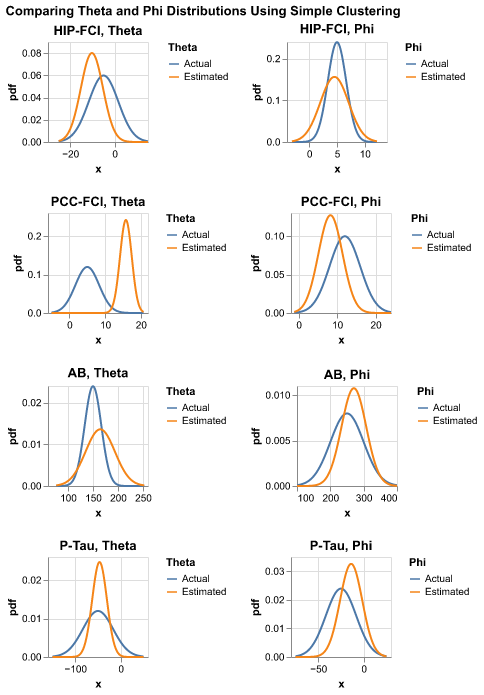
\includegraphics[width=5.04167in,height=7.375in]{estDistParams_files/figure-pdf/fig-estdistparamscopkm-output-1.png}

}

\caption{\label{fig-estdistparamscopkm}Comparing Theta and Phi
Distributions Using Constrained K-Means}

\end{figure}%

It turns out the result is not very desriable.

\section{Conjugate Priors}\label{sec-conjugate-priors}

The second method we may utilize is conjugate priors. Conjugacy occurs
when the posterior distribution is in the same family of distribution as
the prior distribution, but with new parameter values.

Why conjugacy is important? Because without it, one has to do the
integration, which oftentimes is hard.

Three major conjugate families:

\begin{itemize}
\tightlist
\item
  Beta-Binomial
\item
  Gamma-Poisson
\item
  Normal-Normal
\end{itemize}

In our example, we assume that the measurement data for each biomarker
follows a normal distribution; however, we do not know the exact \(\mu\)
and \(\sigma\). Our job is to estimate the two parameters for each
biomarker based on the data we have.

According to
\href{https://statswithr.github.io/book/inference-and-decision-making-with-multiple-parameters.html\#sec:normal-gamma}{\emph{An
Introduction to Bayesian Thinking}} by Clyde et al. (2022), if the data
comes from a normal distribution with unknown \(\mu\) and \(\sigma\),
the conjugate prior for \(\mu\) has a normal distribution with mean
\(m_0\) and variance \(\frac{\sigma^2}{n_0}\). The conjugate prior for
\(\frac{1}{\sigma^2}\) has a Gamma distribution with shape
\(\frac{v_0}{2}\) and rate \(\frac{v_0 s_0^{2}}{2}\) where

\begin{itemize}
\tightlist
\item
  \(m_0\): prior estimate of \(\mu\).
\item
  \(n_0\): how strongly is the prior belief in \(m_0\) is held.
\item
  \(s_0^2\): prior estimate of \(\sigma^2\).
\item
  \(v_0\): prior degress of freedome, influencing the certainty of
  \(s_0^2\).
\end{itemize}

That is to say:

\[\mu | \sigma^2 \sim \mathcal{N}(m_0, \sigma^2/n_0)\]

\[1/\sigma^2 \sim Gamma\left(\frac{v_0}{2}, \frac{v_0 s_0^2}{2} \right)\]

Combined, we have:

\[(\mu, 1/\sigma^2) \sim NormalGamma(m_0, n_0, s_0^2, v_0)\]

The posterior also follows a Normal-Gamma distribution:

\[(\mu, 1/\sigma^2) | data \sim NormalGamma(m_n, n_n, s_n^2, v_n)\]

More specifically

\[1/\sigma^2 | data \sim Gamma(v_n/2, s_n^2 v_n/2)\]

\[\mu | data, \sigma^2 \sim \mathcal{N}(m_n, \sigma^2/n_n)\]

Based on the above two equations, we know that the mean of posterior
mean is \(m_n\) and the mean of the posterior variance is
\((s_n^2 v_n/2)/(v_n/2)\). This is beceause the expected value of
\(Gamma(\alpha, \beta)\) is \(\frac{\alpha}{\beta}\).

where

\begin{itemize}
\tightlist
\item
  \(m_n\): posterior mean, mode, and median for \(\mu\)
\item
  \(n_n\): posterior sample size
\item
  \(s_n^2\): posterior variance
\item
  \(v_n\): posterior degrees of freedome
\end{itemize}

The updating rules to get the new hyper-parameters:

\[m_n = \frac{n}{n+n_0} \bar{y} + \frac{n_0}{n+n_0}m_0\]

\[n_n = n_0 + n\]

\[v_n = v_0 + n\]

\[s_n^2 = \frac{1}{v_n}\left[s^2(n-1) + s_0^2v_0 + \frac{n_0n}{n_n}(\bar{y}-m_0)^2\right]\]

where

\begin{itemize}
\tightlist
\item
  \(n\): sample size
\item
  \(\bar{y}\): sample mean
\item
  \(s^2\): sample variance
\end{itemize}

\begin{tcolorbox}[enhanced jigsaw, bottomrule=.15mm, colback=white, bottomtitle=1mm, titlerule=0mm, arc=.35mm, breakable, rightrule=.15mm, opacityback=0, leftrule=.75mm, opacitybacktitle=0.6, colframe=quarto-callout-tip-color-frame, coltitle=black, toptitle=1mm, colbacktitle=quarto-callout-tip-color!10!white, title=\textcolor{quarto-callout-tip-color}{\faLightbulb}\hspace{0.5em}{Tip}, left=2mm, toprule=.15mm]

To apply the algorithm of conjugate priors, we assume we already know
\(S\) and \(k_j\), alongside biomarker measurement (\(X_{nj}\)). Based
on \(S\) and \(k_j\), we can infer whether a biomarker is affected by
the disease or not.

\end{tcolorbox}

\begin{Shaded}
\begin{Highlighting}[]
\KeywordTok{def}\NormalTok{ estimate\_params\_exact(m0, n0, s0\_sq, v0, data):}
    \CommentTok{\textquotesingle{}\textquotesingle{}\textquotesingle{}This is to estimate means and vars based on conjugate priors}
\CommentTok{    Inputs:}
\CommentTok{        {-} data: a vector of measurements }
\CommentTok{        {-} m0: prior estimate of $\textbackslash{}mu$.}
\CommentTok{        {-} n0: how strongly is the prior belief in $m\_0$ is held.}
\CommentTok{        {-} s0\_sq: prior estimate of $\textbackslash{}sigma\^{}2$.}
\CommentTok{        {-} v0: prior degress of freedome, influencing the certainty of $s\_0\^{}2$.}

\CommentTok{    Outputs:}
\CommentTok{        {-} mu estiate, std estimate}
\CommentTok{    \textquotesingle{}\textquotesingle{}\textquotesingle{}}
    \CommentTok{\# Data summary}
\NormalTok{    sample\_mean }\OperatorTok{=}\NormalTok{ np.mean(data)}
\NormalTok{    sample\_size }\OperatorTok{=} \BuiltInTok{len}\NormalTok{(data)}
\NormalTok{    sample\_var }\OperatorTok{=}\NormalTok{ np.var(data, ddof}\OperatorTok{=}\DecValTok{1}\NormalTok{)  }\CommentTok{\# ddof=1 for unbiased estimator}

    \CommentTok{\# Update hyperparameters for the Normal{-}Inverse Gamma posterior}
\NormalTok{    updated\_m0 }\OperatorTok{=}\NormalTok{ (n0 }\OperatorTok{*}\NormalTok{ m0 }\OperatorTok{+}\NormalTok{ sample\_size }\OperatorTok{*}\NormalTok{ sample\_mean) }\OperatorTok{/}\NormalTok{ (n0 }\OperatorTok{+}\NormalTok{ sample\_size)}
\NormalTok{    updated\_n0 }\OperatorTok{=}\NormalTok{ n0 }\OperatorTok{+}\NormalTok{ sample\_size}
\NormalTok{    updated\_v0 }\OperatorTok{=}\NormalTok{ v0 }\OperatorTok{+}\NormalTok{ sample\_size}
\NormalTok{    updated\_s0\_sq }\OperatorTok{=}\NormalTok{ (}\DecValTok{1} \OperatorTok{/}\NormalTok{ updated\_v0) }\OperatorTok{*}\NormalTok{ ((sample\_size }\OperatorTok{{-}} \DecValTok{1}\NormalTok{) }\OperatorTok{*}\NormalTok{ sample\_var }\OperatorTok{+}\NormalTok{ v0 }\OperatorTok{*}\NormalTok{ s0\_sq }\OperatorTok{+}
\NormalTok{                                        (n0 }\OperatorTok{*}\NormalTok{ sample\_size }\OperatorTok{/}\NormalTok{ updated\_n0) }\OperatorTok{*}\NormalTok{ (sample\_mean }\OperatorTok{{-}}\NormalTok{ m0)}\OperatorTok{**}\DecValTok{2}\NormalTok{)}
\NormalTok{    updated\_alpha }\OperatorTok{=}\NormalTok{ updated\_v0}\OperatorTok{/}\DecValTok{2}
\NormalTok{    updated\_beta }\OperatorTok{=}\NormalTok{ updated\_v0}\OperatorTok{*}\NormalTok{updated\_s0\_sq}\OperatorTok{/}\DecValTok{2}

    \CommentTok{\# Posterior estimates}
\NormalTok{    mu\_posterior\_mean }\OperatorTok{=}\NormalTok{ updated\_m0}
\NormalTok{    sigma\_squared\_posterior\_mean }\OperatorTok{=}\NormalTok{ updated\_beta}\OperatorTok{/}\NormalTok{updated\_alpha}

\NormalTok{    mu\_estimation }\OperatorTok{=}\NormalTok{ mu\_posterior\_mean}
\NormalTok{    std\_estimation }\OperatorTok{=}\NormalTok{ np.sqrt(sigma\_squared\_posterior\_mean)}

    \ControlFlowTok{return}\NormalTok{ mu\_estimation, std\_estimation}

\KeywordTok{def}\NormalTok{ get\_theta\_phi\_conjugate\_priors(biomarkers, data\_we\_have, theta\_phi\_kmeans):}
    \CommentTok{\textquotesingle{}\textquotesingle{}\textquotesingle{}To get estimated parameters, returns a hashmap}
\CommentTok{    Input:}
\CommentTok{    {-} biomarkers: biomarkers }
\CommentTok{    {-} data\_we\_have: participants data filled with initial or updated participant\_stages}
\CommentTok{    {-} theta\_phi\_kmeans: a hashmap of dicts, which are the prior theta and phi values}
\CommentTok{        obtained from the initial constrained kmeans algorithm}

\CommentTok{    Output: }
\CommentTok{    {-} a hashmap of dictionaries. Key is biomarker name and value is a dictionary.}
\CommentTok{    Each dictionary contains the theta and phi mean/std values for a specific biomarker. }
\CommentTok{    \textquotesingle{}\textquotesingle{}\textquotesingle{}}
    \CommentTok{\# empty list of dictionaries to store the estimates}
\NormalTok{    hashmap\_of\_means\_stds\_estimate\_dicts }\OperatorTok{=}\NormalTok{ \{\}}

    \ControlFlowTok{for}\NormalTok{ biomarker }\KeywordTok{in}\NormalTok{ biomarkers:}
        \CommentTok{\# Initialize dictionary outside the inner loop}
\NormalTok{        dic }\OperatorTok{=}\NormalTok{ \{}\StringTok{\textquotesingle{}biomarker\textquotesingle{}}\NormalTok{: biomarker\}}
        \ControlFlowTok{for}\NormalTok{ affected }\KeywordTok{in}\NormalTok{ [}\StringTok{\textquotesingle{}affected\textquotesingle{}}\NormalTok{, }\StringTok{\textquotesingle{}not\_affected\textquotesingle{}}\NormalTok{]:}
\NormalTok{            data\_full }\OperatorTok{=}\NormalTok{ data\_we\_have[(data\_we\_have.biomarker }\OperatorTok{==}\NormalTok{ biomarker) }\OperatorTok{\&}\NormalTok{ (}
\NormalTok{                data\_we\_have.affected\_or\_not }\OperatorTok{==}\NormalTok{ affected)]}
            \ControlFlowTok{if} \BuiltInTok{len}\NormalTok{(data\_full) }\OperatorTok{\textgreater{}} \DecValTok{1}\NormalTok{:}
\NormalTok{                measurements }\OperatorTok{=}\NormalTok{ data\_full.measurement}
\NormalTok{                s0\_sq }\OperatorTok{=}\NormalTok{ np.var(measurements, ddof}\OperatorTok{=}\DecValTok{1}\NormalTok{)}
\NormalTok{                m0 }\OperatorTok{=}\NormalTok{ np.mean(measurements)}
\NormalTok{                mu\_estimate, std\_estimate }\OperatorTok{=}\NormalTok{ estimate\_params\_exact(}
\NormalTok{                    m0}\OperatorTok{=}\NormalTok{m0, n0}\OperatorTok{=}\DecValTok{1}\NormalTok{, s0\_sq}\OperatorTok{=}\NormalTok{s0\_sq, v0}\OperatorTok{=}\DecValTok{1}\NormalTok{, data}\OperatorTok{=}\NormalTok{measurements)}
                \ControlFlowTok{if}\NormalTok{ affected }\OperatorTok{==} \StringTok{\textquotesingle{}affected\textquotesingle{}}\NormalTok{:}
\NormalTok{                    dic[}\StringTok{\textquotesingle{}theta\_mean\textquotesingle{}}\NormalTok{] }\OperatorTok{=}\NormalTok{ mu\_estimate}
\NormalTok{                    dic[}\StringTok{\textquotesingle{}theta\_std\textquotesingle{}}\NormalTok{] }\OperatorTok{=}\NormalTok{ std\_estimate}
                \ControlFlowTok{else}\NormalTok{:}
\NormalTok{                    dic[}\StringTok{\textquotesingle{}phi\_mean\textquotesingle{}}\NormalTok{] }\OperatorTok{=}\NormalTok{ mu\_estimate}
\NormalTok{                    dic[}\StringTok{\textquotesingle{}phi\_std\textquotesingle{}}\NormalTok{] }\OperatorTok{=}\NormalTok{ std\_estimate}
            \CommentTok{\# If there is only one observation or not observation at all, resort to theta\_phi\_kmeans}
            \CommentTok{\# YES, IT IS POSSIBLE THAT DATA\_FULL HERE IS NULL}
            \CommentTok{\# For example, if a biomarker indicates stage of (num\_biomarkers), but all participants\textquotesingle{} stages}
            \CommentTok{\# are smaller than that stage; so that for all participants, this biomarker is not affected}
            \ControlFlowTok{else}\NormalTok{:}
                \BuiltInTok{print}\NormalTok{(}\StringTok{\textquotesingle{}not enough data here, so we have to use theta phi estimates from constrained kmeans\textquotesingle{}}\NormalTok{)}
                \CommentTok{\# print(theta\_phi\_kmeans)}
                \ControlFlowTok{if}\NormalTok{ affected }\OperatorTok{==} \StringTok{\textquotesingle{}affected\textquotesingle{}}\NormalTok{:}
\NormalTok{                    dic[}\StringTok{\textquotesingle{}theta\_mean\textquotesingle{}}\NormalTok{] }\OperatorTok{=}\NormalTok{ theta\_phi\_kmeans[biomarker][}\StringTok{\textquotesingle{}theta\_mean\textquotesingle{}}\NormalTok{]}
\NormalTok{                    dic[}\StringTok{\textquotesingle{}theta\_std\textquotesingle{}}\NormalTok{] }\OperatorTok{=}\NormalTok{ theta\_phi\_kmeans[biomarker][}\StringTok{\textquotesingle{}theta\_std\textquotesingle{}}\NormalTok{]}
                \ControlFlowTok{else}\NormalTok{:}
\NormalTok{                    dic[}\StringTok{\textquotesingle{}phi\_mean\textquotesingle{}}\NormalTok{] }\OperatorTok{=}\NormalTok{ theta\_phi\_kmeans[biomarker][}\StringTok{\textquotesingle{}phi\_mean\textquotesingle{}}\NormalTok{]}
\NormalTok{                    dic[}\StringTok{\textquotesingle{}phi\_std\textquotesingle{}}\NormalTok{] }\OperatorTok{=}\NormalTok{ theta\_phi\_kmeans[biomarker][}\StringTok{\textquotesingle{}phi\_std\textquotesingle{}}\NormalTok{]}
        \CommentTok{\# print(f"biomarker \{biomarker\} done!")}
\NormalTok{        hashmap\_of\_means\_stds\_estimate\_dicts[biomarker] }\OperatorTok{=}\NormalTok{ dic}
    \ControlFlowTok{return}\NormalTok{ hashmap\_of\_means\_stds\_estimate\_dicts}
\end{Highlighting}
\end{Shaded}

\begin{Shaded}
\begin{Highlighting}[]
\NormalTok{conjugate\_prior\_theta\_phi }\OperatorTok{=}\NormalTok{ get\_theta\_phi\_conjugate\_priors(}
\NormalTok{    biomarkers }\OperatorTok{=}\NormalTok{ biomarkers, }
\NormalTok{    data\_we\_have }\OperatorTok{=}\NormalTok{ df, }
\NormalTok{    theta\_phi\_kmeans }\OperatorTok{=}\NormalTok{ cop\_kmeans\_estimates}
\NormalTok{)}
\NormalTok{cp\_df }\OperatorTok{=}\NormalTok{ pd.DataFrame.from\_dict(conjugate\_prior\_theta\_phi, orient}\OperatorTok{=}\StringTok{\textquotesingle{}index\textquotesingle{}}\NormalTok{)}
\NormalTok{cp\_df.reset\_index(drop}\OperatorTok{=}\VariableTok{True}\NormalTok{, inplace}\OperatorTok{=}\VariableTok{True}\NormalTok{)}
\NormalTok{cp\_df}
\end{Highlighting}
\end{Shaded}

\begin{longtable}[]{@{}llllll@{}}
\toprule\noalign{}
& biomarker & theta\_mean & theta\_std & phi\_mean & phi\_std \\
\midrule\noalign{}
\endhead
\bottomrule\noalign{}
\endlastfoot
0 & HIP-FCI & -5.378366 & 7.233991 & 5.092800 & 1.514402 \\
1 & PCC-FCI & 5.521792 & 2.777207 & 12.071769 & 3.671679 \\
2 & AB & 151.143708 & 14.806694 & 251.973564 & 51.382188 \\
3 & P-Tau & -41.768257 & 34.857945 & -24.739527 & 14.928907 \\
4 & MMSE & 23.122406 & 2.446874 & 28.049683 & 0.718493 \\
5 & ADAS & -19.633304 & 4.582900 & -5.902198 & 1.278311 \\
6 & HIP-GMI & 0.425625 & 0.272876 & 0.379542 & 0.235348 \\
7 & AVLT-Sum & 21.664360 & 3.755735 & 40.700638 & 14.480463 \\
8 & FUS-GMI & 0.482745 & 0.055585 & 0.590434 & 0.063730 \\
9 & FUS-FCI & -18.566905 & 5.781937 & -9.648705 & 3.099195 \\
\end{longtable}

\begin{tcolorbox}[enhanced jigsaw, bottomrule=.15mm, colback=white, bottomtitle=1mm, titlerule=0mm, arc=.35mm, breakable, rightrule=.15mm, opacityback=0, leftrule=.75mm, opacitybacktitle=0.6, colframe=quarto-callout-note-color-frame, coltitle=black, toptitle=1mm, colbacktitle=quarto-callout-note-color!10!white, title=\textcolor{quarto-callout-note-color}{\faInfo}\hspace{0.5em}{Note}, left=2mm, toprule=.15mm]

When we estimate \(\theta\) and \(\phi\) using conjugate priors, we need
to use the result from constrained kmeans as a fall back because it is
possible that for a specific biomarker, either the \texttt{affected} or
the \texttt{not\_affected} group is empty. If that is the case, we are
not able to estimate relevant parameters and have to resort to the
fallback result.

\end{tcolorbox}

\begin{Shaded}
\begin{Highlighting}[]
\NormalTok{make\_chart(}
\NormalTok{    biomarkers[}\DecValTok{0}\NormalTok{:}\DecValTok{4}\NormalTok{], }
\NormalTok{    cp\_df, }
\NormalTok{    truth\_df, }
\NormalTok{    title }\OperatorTok{=} \StringTok{"Comparing Theta and Phi Distributions Using Conjugate Priors"}
\NormalTok{)}
\end{Highlighting}
\end{Shaded}

\begin{figure}[H]

\centering{

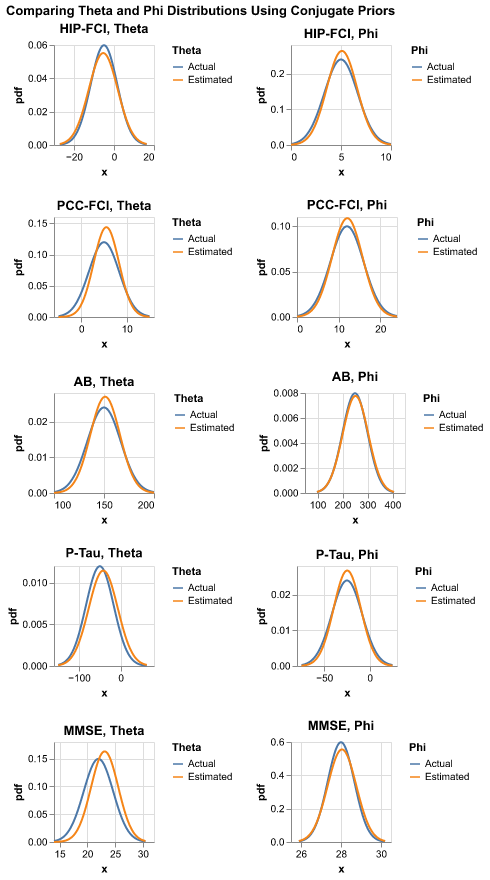
\includegraphics[width=5.10417in,height=7.33333in]{estDistParams_files/figure-pdf/fig-estdistparamscp-output-1.png}

}

\caption{\label{fig-estdistparamscp}Comparing Theta and Phi
Distributions Using Conjugate Prior}

\end{figure}%

\section{Soft K-Means}\label{sec-soft-kmeans}

Conjugate Priors assumes we know \(k_j\), which often times is not
already known. Constrained K-Means is only taking advantage of
\(X_{nj}\) and whether participants are diseased or not, leaving \(S\),
which is known to us, unexploited.

Soft K-Means is a good alternative to these two because it utilizes
\(S\) while at the same time not assuming we know \(k_j\).

The logic of soft-kmeans is this;

\begin{enumerate}
\def\labelenumi{\arabic{enumi}.}
\tightlist
\item
  If a participant is diseased, we iterate through all possible disease
  stages, and calculate the associated likelihood using
  Equation~\ref{eq-known-kj}. We then normalize these likelihoods to
  obtain the estimated probability of this participant being at each
  stage. For example, if there are three possible stages, and the
  associated likelihoods are \texttt{{[}1,\ 3,\ 6{]}}, then the
  normalized likelihoods would be \texttt{{[}0.1,\ 0.3,\ 0.6{]}}.
\end{enumerate}

\begin{tcolorbox}[enhanced jigsaw, bottomrule=.15mm, colback=white, bottomtitle=1mm, titlerule=0mm, arc=.35mm, breakable, rightrule=.15mm, opacityback=0, leftrule=.75mm, opacitybacktitle=0.6, colframe=quarto-callout-tip-color-frame, coltitle=black, toptitle=1mm, colbacktitle=quarto-callout-tip-color!10!white, title=\textcolor{quarto-callout-tip-color}{\faLightbulb}\hspace{0.5em}{Tip}, left=2mm, toprule=.15mm]

You may wonder how we can use Equation~\ref{eq-known-kj} when we do not
know \(\theta\) and \(\phi\) yet (which is exactly what we are trying to
do!). If you notice this, it is a very keen observation!.

If fact, we are going to use the estimated \(\theta\) and \(\phi\) we
obtained above using constrained K-Means.

\end{tcolorbox}

\begin{enumerate}
\def\labelenumi{\arabic{enumi}.}
\setcounter{enumi}{1}
\tightlist
\item
  For each biomarker \(n\), we obtain \(S_n\) based on \(S\). Then we
  iterate through all participants. If this participant is healthy, we
  include their biomarker measurement in \texttt{cluster\_phi}. If this
  participant is diseased, we compare between \(P_{\theta}\) and
  \(P_{\phi}\). If \(S_n = 2\), then \(P_{\theta} = 0.1 + 0.3 = 0.4\)
  and \(P_{\phi} = 0.6\). Because \(P_{\phi}\) is larger, we include
  this participant's biomarker measurement in \texttt{cluster\_phi}.
  When the iteration through participants is done, we can calculate the
  mean and standard deviation of each cluster.
\end{enumerate}

\begin{tcolorbox}[enhanced jigsaw, bottomrule=.15mm, colback=white, bottomtitle=1mm, titlerule=0mm, arc=.35mm, breakable, rightrule=.15mm, opacityback=0, leftrule=.75mm, opacitybacktitle=0.6, colframe=quarto-callout-tip-color-frame, coltitle=black, toptitle=1mm, colbacktitle=quarto-callout-tip-color!10!white, title=\textcolor{quarto-callout-tip-color}{\faLightbulb}\hspace{0.5em}{Tip}, left=2mm, toprule=.15mm]

If \(P_{\theta} =  P_{\phi}\), we randomly assign this participant's
biomarker measurement to a cluster.

\end{tcolorbox}

\begin{Shaded}
\begin{Highlighting}[]
\KeywordTok{def}\NormalTok{ compute\_single\_measurement\_likelihood(theta\_phi, biomarker, affected, measurement):}
    \CommentTok{\textquotesingle{}\textquotesingle{}\textquotesingle{}Computes the likelihood of the measurement value of a single biomarker}

\CommentTok{    We know the normal distribution defined by either theta or phi}
\CommentTok{    and we know the measurement. This will give us the probability}
\CommentTok{    of this given measurement value. }

\CommentTok{    input:}
\CommentTok{    {-} theta\_phi: the dictionary containing theta and phi values for each biomarker}
\CommentTok{    {-} biomarker: an integer between 0 and 9 }
\CommentTok{    {-} affected: boolean }
\CommentTok{    {-} measurement: the observed value for a biomarker in a specific participant}

\CommentTok{    output: a scalar}
\CommentTok{    \textquotesingle{}\textquotesingle{}\textquotesingle{}}
\NormalTok{    biomarker\_dict }\OperatorTok{=}\NormalTok{ theta\_phi[biomarker]}
\NormalTok{    mu }\OperatorTok{=}\NormalTok{ biomarker\_dict[}\StringTok{\textquotesingle{}theta\_mean\textquotesingle{}}\NormalTok{] }\ControlFlowTok{if}\NormalTok{ affected }\ControlFlowTok{else}\NormalTok{ biomarker\_dict[}\StringTok{\textquotesingle{}phi\_mean\textquotesingle{}}\NormalTok{]}
\NormalTok{    std }\OperatorTok{=}\NormalTok{ biomarker\_dict[}\StringTok{\textquotesingle{}theta\_std\textquotesingle{}}\NormalTok{] }\ControlFlowTok{if}\NormalTok{ affected }\ControlFlowTok{else}\NormalTok{ biomarker\_dict[}\StringTok{\textquotesingle{}phi\_std\textquotesingle{}}\NormalTok{]}
\NormalTok{    var }\OperatorTok{=}\NormalTok{ std}\OperatorTok{**}\DecValTok{2}
    \ControlFlowTok{if}\NormalTok{ var }\OperatorTok{\textless{}=} \BuiltInTok{int}\NormalTok{(}\DecValTok{0}\NormalTok{) }\KeywordTok{or}\NormalTok{ np.isnan(measurement) }\KeywordTok{or}\NormalTok{ np.isnan(mu):}
        \BuiltInTok{print}\NormalTok{(}\SpecialStringTok{f"Invalid values: measurement: }\SpecialCharTok{\{}\NormalTok{measurement}\SpecialCharTok{\}}\SpecialStringTok{, mu: }\SpecialCharTok{\{}\NormalTok{mu}\SpecialCharTok{\}}\SpecialStringTok{, var: }\SpecialCharTok{\{}\NormalTok{var}\SpecialCharTok{\}}\SpecialStringTok{"}\NormalTok{)}
\NormalTok{        likelihood }\OperatorTok{=}\NormalTok{ np.exp(}\OperatorTok{{-}}\NormalTok{(measurement }\OperatorTok{{-}}\NormalTok{ mu)}\OperatorTok{**}\DecValTok{2} \OperatorTok{/}
\NormalTok{                            (}\DecValTok{2} \OperatorTok{*}\NormalTok{ var)) }\OperatorTok{/}\NormalTok{ np.sqrt(}\DecValTok{2} \OperatorTok{*}\NormalTok{ np.pi }\OperatorTok{*}\NormalTok{ var)}
    \ControlFlowTok{else}\NormalTok{:}
\NormalTok{        likelihood }\OperatorTok{=}\NormalTok{ np.exp(}\OperatorTok{{-}}\NormalTok{(measurement }\OperatorTok{{-}}\NormalTok{ mu)}\OperatorTok{**}\DecValTok{2} \OperatorTok{/}
\NormalTok{                            (}\DecValTok{2} \OperatorTok{*}\NormalTok{ var)) }\OperatorTok{/}\NormalTok{ np.sqrt(}\DecValTok{2} \OperatorTok{*}\NormalTok{ np.pi }\OperatorTok{*}\NormalTok{ var)}
    \ControlFlowTok{return}\NormalTok{ likelihood}

\KeywordTok{def}\NormalTok{ fill\_up\_kj\_and\_affected(pdata, k\_j):}
    \CommentTok{\textquotesingle{}\textquotesingle{}\textquotesingle{}Fill up a single participant\textquotesingle{}s data using k\_j; basically add two columns: }
\CommentTok{    k\_j and affected}
\CommentTok{    Note that this function assumes that pdata already has the S\_n column}

\CommentTok{    Input:}
\CommentTok{    {-} pdata: a dataframe of ten biomarker values for a specific participant }
\CommentTok{    {-} k\_j: a scalar}
\CommentTok{    \textquotesingle{}\textquotesingle{}\textquotesingle{}}
\NormalTok{    data }\OperatorTok{=}\NormalTok{ pdata.copy()}
\NormalTok{    data[}\StringTok{\textquotesingle{}k\_j\textquotesingle{}}\NormalTok{] }\OperatorTok{=}\NormalTok{ k\_j}
\NormalTok{    data[}\StringTok{\textquotesingle{}affected\textquotesingle{}}\NormalTok{] }\OperatorTok{=}\NormalTok{ data.}\BuiltInTok{apply}\NormalTok{(}\KeywordTok{lambda}\NormalTok{ row: row.k\_j }\OperatorTok{\textgreater{}=}\NormalTok{ row.S\_n, axis}\OperatorTok{=}\DecValTok{1}\NormalTok{)}
    \ControlFlowTok{return}\NormalTok{ data}

\KeywordTok{def}\NormalTok{ compute\_likelihood(pdata, k\_j, theta\_phi):}
    \CommentTok{\textquotesingle{}\textquotesingle{}\textquotesingle{}}
\CommentTok{    This function computes the likelihood of seeing this sequence of biomarker values }
\CommentTok{    for a specific participant, assuming that this participant is at stage k\_j}
\CommentTok{    \textquotesingle{}\textquotesingle{}\textquotesingle{}}
\NormalTok{    data }\OperatorTok{=}\NormalTok{ fill\_up\_kj\_and\_affected(pdata, k\_j)}
\NormalTok{    likelihood }\OperatorTok{=} \DecValTok{1}
    \ControlFlowTok{for}\NormalTok{ i, row }\KeywordTok{in}\NormalTok{ data.iterrows():}
\NormalTok{        biomarker }\OperatorTok{=}\NormalTok{ row[}\StringTok{\textquotesingle{}biomarker\textquotesingle{}}\NormalTok{]}
\NormalTok{        measurement }\OperatorTok{=}\NormalTok{ row[}\StringTok{\textquotesingle{}measurement\textquotesingle{}}\NormalTok{]}
\NormalTok{        affected }\OperatorTok{=}\NormalTok{ row[}\StringTok{\textquotesingle{}affected\textquotesingle{}}\NormalTok{]}
\NormalTok{        likelihood }\OperatorTok{*=}\NormalTok{ compute\_single\_measurement\_likelihood(}
\NormalTok{            theta\_phi, biomarker, affected, measurement)}
    \ControlFlowTok{return}\NormalTok{ likelihood}

\KeywordTok{def}\NormalTok{ obtain\_participants\_hashmap(}
\NormalTok{        data, }
\NormalTok{        prior\_theta\_phi\_estimates,}
\NormalTok{):}
    \CommentTok{"""}
\CommentTok{    Input:}
\CommentTok{        {-} data: a pd.dataframe. For exrample, 150|200\_3.csv}
\CommentTok{        {-} prior\_theta\_phi\_estimates, a hashmap of dicts. }
\CommentTok{            This is the result from constrained kmeans }
\CommentTok{    }
\CommentTok{    Output: }
\CommentTok{        {-} hashmap: a dictionary whose key is participant id}
\CommentTok{            and value value is a dict whose key is stage }
\CommentTok{            and value is normalized likelihood}
\CommentTok{    """}
    \CommentTok{\# initialize hashmap\_of\_normalized\_stage\_likelihood\_dicts}
\NormalTok{    participants\_hashmap }\OperatorTok{=}\NormalTok{ \{\}}
\NormalTok{    non\_diseased\_participants }\OperatorTok{=}\NormalTok{ data[}
\NormalTok{        data.diseased }\OperatorTok{==} \VariableTok{False}\NormalTok{][}\StringTok{\textquotesingle{}participant\textquotesingle{}}\NormalTok{].unique()}
\NormalTok{    disease\_stages }\OperatorTok{=}\NormalTok{ data.S\_n.unique()}
    \ControlFlowTok{for}\NormalTok{ p }\KeywordTok{in}\NormalTok{ data.participant.unique():}
\NormalTok{        dic }\OperatorTok{=}\NormalTok{ defaultdict(}\BuiltInTok{int}\NormalTok{)}
\NormalTok{        pdata }\OperatorTok{=}\NormalTok{ data[data.participant }\OperatorTok{==}\NormalTok{ p].reset\_index(drop }\OperatorTok{=} \VariableTok{True}\NormalTok{)}
        \ControlFlowTok{if}\NormalTok{ p }\KeywordTok{in}\NormalTok{ non\_diseased\_participants:}
\NormalTok{            dic[}\DecValTok{0}\NormalTok{] }\OperatorTok{=} \DecValTok{1}
        \ControlFlowTok{else}\NormalTok{:}
            \ControlFlowTok{for}\NormalTok{ k\_j }\KeywordTok{in}\NormalTok{ disease\_stages:}
\NormalTok{                kj\_ll }\OperatorTok{=}\NormalTok{ compute\_likelihood(pdata, k\_j, prior\_theta\_phi\_estimates)}
\NormalTok{                dic[k\_j] }\OperatorTok{=}\NormalTok{ kj\_ll}
            \CommentTok{\# likelihood sum}
\NormalTok{            sum\_ll }\OperatorTok{=} \BuiltInTok{sum}\NormalTok{(dic.values())}
\NormalTok{            epsilon }\OperatorTok{=} \FloatTok{1e{-}10}
            \ControlFlowTok{if}\NormalTok{ sum\_ll }\OperatorTok{==} \DecValTok{0}\NormalTok{:}
\NormalTok{                sum\_ll }\OperatorTok{=}\NormalTok{ epsilon}
\NormalTok{            normalized\_lls }\OperatorTok{=}\NormalTok{ [l}\OperatorTok{/}\NormalTok{sum\_ll }\ControlFlowTok{for}\NormalTok{ l }\KeywordTok{in}\NormalTok{ dic.values()]}
\NormalTok{            normalized\_ll\_dict }\OperatorTok{=} \BuiltInTok{dict}\NormalTok{(}\BuiltInTok{zip}\NormalTok{(disease\_stages, normalized\_lls))}
\NormalTok{            participants\_hashmap[p] }\OperatorTok{=}\NormalTok{ normalized\_ll\_dict}
    \ControlFlowTok{return}\NormalTok{ participants\_hashmap }

\KeywordTok{def}\NormalTok{ calc\_soft\_kmeans\_for\_biomarker(}
\NormalTok{        data,}
\NormalTok{        biomarker,}
\NormalTok{        participants\_hashmap}

\NormalTok{):}
    \CommentTok{"""obtain theta, phi estimates using soft kmeans for a single biomarker}
\CommentTok{    Inputs:}
\CommentTok{        {-} data: a pd.dataframe. For example, 150|200\_3.csv}
\CommentTok{        {-} biomarker: a str, a certain biomarker name}
\CommentTok{        {-} hashmap: a dict, returned result of obtain\_hashmap()}
\CommentTok{    Outputs:}
\CommentTok{        {-} theta\_mean, theta\_std, phi\_mean, phi\_std, a tuple of floats}
\CommentTok{    """}
\NormalTok{    non\_diseased\_participants }\OperatorTok{=}\NormalTok{ data[}
\NormalTok{        data.diseased }\OperatorTok{==} \VariableTok{False}\NormalTok{][}\StringTok{\textquotesingle{}participant\textquotesingle{}}\NormalTok{].unique()}
\NormalTok{    disease\_stages }\OperatorTok{=}\NormalTok{ data.S\_n.unique()}
     \CommentTok{\# DataFrame for this biomarker}
\NormalTok{    biomarker\_df }\OperatorTok{=}\NormalTok{ data[}
\NormalTok{        data[}\StringTok{\textquotesingle{}biomarker\textquotesingle{}}\NormalTok{] }\OperatorTok{==}\NormalTok{ biomarker].reset\_index(}
\NormalTok{            drop}\OperatorTok{=}\VariableTok{True}\NormalTok{).sort\_values(}
\NormalTok{                by }\OperatorTok{=} \StringTok{\textquotesingle{}participant\textquotesingle{}}\NormalTok{, ascending }\OperatorTok{=} \VariableTok{True}\NormalTok{)}
    \CommentTok{\# Extract measurements}
\NormalTok{    measurements }\OperatorTok{=}\NormalTok{ np.array(biomarker\_df[}\StringTok{\textquotesingle{}measurement\textquotesingle{}}\NormalTok{])}

\NormalTok{    this\_biomarker\_order }\OperatorTok{=}\NormalTok{ biomarker\_df.S\_n[}\DecValTok{0}\NormalTok{]}

\NormalTok{    affected\_cluster }\OperatorTok{=}\NormalTok{ []}
\NormalTok{    non\_affected\_cluster }\OperatorTok{=}\NormalTok{ []}

    \ControlFlowTok{for}\NormalTok{ p }\KeywordTok{in}\NormalTok{ data.participant.unique():}
        \ControlFlowTok{if}\NormalTok{ p }\KeywordTok{in}\NormalTok{ non\_diseased\_participants:}
\NormalTok{            non\_affected\_cluster.append(measurements[p])}
        \ControlFlowTok{else}\NormalTok{:}
\NormalTok{            normalized\_ll\_dict }\OperatorTok{=}\NormalTok{ participants\_hashmap[p]}
\NormalTok{            affected\_prob }\OperatorTok{=} \BuiltInTok{sum}\NormalTok{(}
\NormalTok{                normalized\_ll\_dict[}
\NormalTok{                    kj] }\ControlFlowTok{for}\NormalTok{ kj }\KeywordTok{in}\NormalTok{ disease\_stages }\ControlFlowTok{if}\NormalTok{ kj }\OperatorTok{\textgreater{}=}\NormalTok{ this\_biomarker\_order)}
\NormalTok{            non\_affected\_prob }\OperatorTok{=} \BuiltInTok{sum}\NormalTok{(}
\NormalTok{                normalized\_ll\_dict[}
\NormalTok{                    kj] }\ControlFlowTok{for}\NormalTok{ kj }\KeywordTok{in}\NormalTok{ disease\_stages }\ControlFlowTok{if}\NormalTok{ kj }\OperatorTok{\textless{}}\NormalTok{ this\_biomarker\_order)}
            \ControlFlowTok{if}\NormalTok{ affected\_prob }\OperatorTok{\textgreater{}}\NormalTok{ non\_affected\_prob:}
\NormalTok{                    affected\_cluster.append(measurements[p])}
            \ControlFlowTok{elif}\NormalTok{ affected\_prob }\OperatorTok{\textless{}}\NormalTok{ non\_affected\_prob:}
\NormalTok{                non\_affected\_cluster.append(measurements[p])}
            \ControlFlowTok{else}\NormalTok{:}
                \CommentTok{\# Assign to either cluster randomly if probabilities are equal}
                \ControlFlowTok{if}\NormalTok{ np.random.random() }\OperatorTok{\textgreater{}} \FloatTok{0.5}\NormalTok{:}
\NormalTok{                    affected\_cluster.append(measurements[p])}
                \ControlFlowTok{else}\NormalTok{:}
\NormalTok{                    non\_affected\_cluster.append(measurements[p])}
    \CommentTok{\# Compute means and standard deviations}
\NormalTok{    theta\_mean }\OperatorTok{=}\NormalTok{ np.mean(affected\_cluster) }\ControlFlowTok{if}\NormalTok{ affected\_cluster }\ControlFlowTok{else}\NormalTok{ np.nan}
\NormalTok{    theta\_std }\OperatorTok{=}\NormalTok{ np.std(affected\_cluster) }\ControlFlowTok{if}\NormalTok{ affected\_cluster }\ControlFlowTok{else}\NormalTok{ np.nan}
\NormalTok{    phi\_mean }\OperatorTok{=}\NormalTok{ np.mean(}
\NormalTok{        non\_affected\_cluster) }\ControlFlowTok{if}\NormalTok{ non\_affected\_cluster }\ControlFlowTok{else}\NormalTok{ np.nan}
\NormalTok{    phi\_std }\OperatorTok{=}\NormalTok{ np.std(non\_affected\_cluster) }\ControlFlowTok{if}\NormalTok{ non\_affected\_cluster }\ControlFlowTok{else}\NormalTok{ np.nan}
    \ControlFlowTok{return}\NormalTok{ theta\_mean, theta\_std, phi\_mean, phi\_std}

\KeywordTok{def}\NormalTok{ cal\_soft\_kmeans\_for\_biomarkers(}
\NormalTok{        data,}
\NormalTok{        participants\_hashmap,}
\NormalTok{        prior\_theta\_phi\_estimates,}
\NormalTok{):}
\NormalTok{    soft\_kmeans\_estimates }\OperatorTok{=}\NormalTok{ \{\}}
\NormalTok{    biomarkers }\OperatorTok{=}\NormalTok{ data.biomarker.unique()}
    \ControlFlowTok{for}\NormalTok{ biomarker }\KeywordTok{in}\NormalTok{ biomarkers:}
\NormalTok{        dic }\OperatorTok{=}\NormalTok{ \{}\StringTok{\textquotesingle{}biomarker\textquotesingle{}}\NormalTok{: biomarker\}}
\NormalTok{        prior }\OperatorTok{=}\NormalTok{ prior\_theta\_phi\_estimates[biomarker]}
\NormalTok{        theta\_mean, theta\_std, phi\_mean, phi\_std }\OperatorTok{=}\NormalTok{ calc\_soft\_kmeans\_for\_biomarker(}
\NormalTok{            data, biomarker, participants\_hashmap}
\NormalTok{        )}
        \ControlFlowTok{if}\NormalTok{ theta\_std }\OperatorTok{==} \DecValTok{0} \KeywordTok{or}\NormalTok{ math.isnan(theta\_std):}
\NormalTok{            theta\_mean }\OperatorTok{=}\NormalTok{ prior[}\StringTok{\textquotesingle{}theta\_mean\textquotesingle{}}\NormalTok{]}
\NormalTok{            theta\_std }\OperatorTok{=}\NormalTok{ prior[}\StringTok{\textquotesingle{}theta\_std\textquotesingle{}}\NormalTok{]}
        \ControlFlowTok{if}\NormalTok{ phi\_std }\OperatorTok{==} \DecValTok{0} \KeywordTok{or}\NormalTok{ math.isnan(phi\_std):}
\NormalTok{            phi\_mean }\OperatorTok{=}\NormalTok{ prior[}\StringTok{\textquotesingle{}phi\_mean\textquotesingle{}}\NormalTok{]}
\NormalTok{            phi\_std }\OperatorTok{=}\NormalTok{ prior[}\StringTok{\textquotesingle{}phi\_std\textquotesingle{}}\NormalTok{]}
\NormalTok{        dic[}\StringTok{\textquotesingle{}theta\_mean\textquotesingle{}}\NormalTok{] }\OperatorTok{=}\NormalTok{ theta\_mean}
\NormalTok{        dic[}\StringTok{\textquotesingle{}theta\_std\textquotesingle{}}\NormalTok{] }\OperatorTok{=}\NormalTok{ theta\_std}
\NormalTok{        dic[}\StringTok{\textquotesingle{}phi\_mean\textquotesingle{}}\NormalTok{] }\OperatorTok{=}\NormalTok{ phi\_mean}
\NormalTok{        dic[}\StringTok{\textquotesingle{}phi\_std\textquotesingle{}}\NormalTok{] }\OperatorTok{=}\NormalTok{ phi\_std}
\NormalTok{        soft\_kmeans\_estimates[biomarker] }\OperatorTok{=}\NormalTok{ dic}
    \ControlFlowTok{return}\NormalTok{ soft\_kmeans\_estimates}
\end{Highlighting}
\end{Shaded}

\begin{Shaded}
\begin{Highlighting}[]
\NormalTok{participants\_hashmap }\OperatorTok{=}\NormalTok{ obtain\_participants\_hashmap(}
\NormalTok{    data }\OperatorTok{=}\NormalTok{ df, }
\NormalTok{    prior\_theta\_phi\_estimates }\OperatorTok{=}\NormalTok{ cop\_kmeans\_estimates,}
\NormalTok{)}

\NormalTok{soft\_kmeans\_estimates }\OperatorTok{=}\NormalTok{ cal\_soft\_kmeans\_for\_biomarkers(}
\NormalTok{        data }\OperatorTok{=}\NormalTok{ df,}
\NormalTok{        participants\_hashmap }\OperatorTok{=}\NormalTok{ participants\_hashmap,}
\NormalTok{        prior\_theta\_phi\_estimates }\OperatorTok{=}\NormalTok{ cop\_kmeans\_estimates,}
\NormalTok{)}
\end{Highlighting}
\end{Shaded}

\begin{Shaded}
\begin{Highlighting}[]
\NormalTok{soft\_kmeans\_estimates\_df }\OperatorTok{=}\NormalTok{ pd.DataFrame.from\_dict(}
\NormalTok{    soft\_kmeans\_estimates, orient}\OperatorTok{=}\StringTok{\textquotesingle{}index\textquotesingle{}}\NormalTok{)}
\NormalTok{soft\_kmeans\_estimates\_df.reset\_index(drop}\OperatorTok{=}\VariableTok{True}\NormalTok{, inplace}\OperatorTok{=}\VariableTok{True}\NormalTok{)}
\NormalTok{soft\_kmeans\_estimates\_df}
\end{Highlighting}
\end{Shaded}

\begin{longtable}[]{@{}llllll@{}}
\toprule\noalign{}
& biomarker & theta\_mean & theta\_std & phi\_mean & phi\_std \\
\midrule\noalign{}
\endhead
\bottomrule\noalign{}
\endlastfoot
0 & HIP-FCI & -5.378366 & 7.232544 & 5.092800 & 1.514369 \\
1 & PCC-FCI & 10.397606 & 3.698129 & 10.572261 & 4.472485 \\
2 & AB & 157.514640 & 19.654237 & 232.546088 & 61.426283 \\
3 & P-Tau & -61.280491 & 21.704315 & -27.032696 & 20.645375 \\
4 & MMSE & 21.478486 & 0.869996 & 27.414771 & 1.956947 \\
5 & ADAS & -23.386222 & 3.249392 & -7.343264 & 4.453207 \\
6 & HIP-GMI & 0.114735 & 0.106857 & 0.385654 & 0.240309 \\
7 & AVLT-Sum & 60.569081 & 6.389012 & 39.177736 & 14.855928 \\
8 & FUS-GMI & 0.478209 & 0.041763 & 0.584511 & 0.067892 \\
9 & FUS-FCI & -19.200644 & 4.688806 & -10.050024 & 3.751844 \\
\end{longtable}

\begin{Shaded}
\begin{Highlighting}[]
\NormalTok{make\_chart(}
\NormalTok{    biomarkers[}\DecValTok{0}\NormalTok{:}\DecValTok{4}\NormalTok{], }
\NormalTok{    soft\_kmeans\_estimates\_df, }
\NormalTok{    truth\_df, }
\NormalTok{    title }\OperatorTok{=} \StringTok{"Comparing Theta and Phi Distributions Using Soft K{-}Means"}
\NormalTok{)}
\end{Highlighting}
\end{Shaded}

\begin{figure}[H]

\centering{

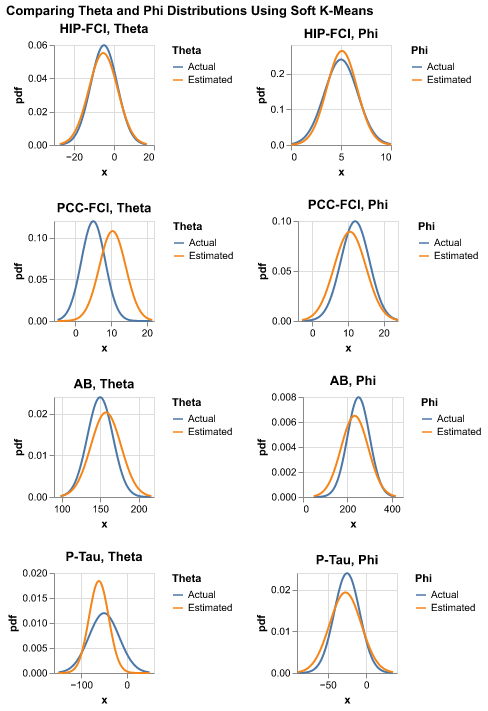
\includegraphics[width=5.08333in,height=7.40625in]{estDistParams_files/figure-pdf/fig-estdistparamsskm-output-1.png}

}

\caption{\label{fig-estdistparamsskm}Comparing Theta and Phi
Distributions Using Soft K-Mean}

\end{figure}%

\section{Conclusion}\label{conclusion}

We compare the above three methods. Constrained k-means has the least
number of prerequisites: it only needs to know whether participants are
healthy or not and biomarker measurements. However, the drawback is that
it might not be very accurate. Conjugate priors are extremely accurate;
however, it requires knowledge of almost everything: besides what is
required by constrained k-kmeans, it also requires \(S\) and \(k_j\).
Soft k-kmeans does not require the knowledge of \(k_j\) and is an
improvement over constrained k-means.

We also noticed that both conjugate priors and soft k-means need to use
the result from constrained k-means as a fallback.

\bookmarksetup{startatroot}

\chapter{Estimate Participant Stages}\label{estimate-participant-stages}

In this chapter, we will do some exercise to have a deeper understanding
of the math equations in Chapter~\ref{sec-calc-ll}.

\section{Challenge}\label{challenge}

Suppos we know \(S, \theta, \phi\). How could we estimate participant
stages?

\begin{Shaded}
\begin{Highlighting}[]
\ImportTok{import}\NormalTok{ pandas }\ImportTok{as}\NormalTok{ pd }
\ImportTok{import}\NormalTok{ numpy }\ImportTok{as}\NormalTok{ np }
\ImportTok{import}\NormalTok{ matplotlib.pyplot }\ImportTok{as}\NormalTok{ plt }
\ImportTok{import}\NormalTok{ json }
\ImportTok{from}\NormalTok{ collections }\ImportTok{import}\NormalTok{ Counter}
\end{Highlighting}
\end{Shaded}

This is the data we have. And we want to know fill the missing column of
\texttt{k\_j}.

\begin{Shaded}
\begin{Highlighting}[]
\NormalTok{output\_dir }\OperatorTok{=} \StringTok{\textquotesingle{}data\textquotesingle{}}
\NormalTok{df }\OperatorTok{=}\NormalTok{ pd.read\_csv(}\SpecialStringTok{f"}\SpecialCharTok{\{}\NormalTok{output\_dir}\SpecialCharTok{\}}\SpecialStringTok{/100|200\_3.csv"}\NormalTok{)}
\NormalTok{real\_stages\_dic }\OperatorTok{=} \BuiltInTok{dict}\NormalTok{(}\BuiltInTok{zip}\NormalTok{(df.participant, df.k\_j))}
\NormalTok{df.drop([}\StringTok{\textquotesingle{}k\_j\textquotesingle{}}\NormalTok{, }\StringTok{\textquotesingle{}affected\_or\_not\textquotesingle{}}\NormalTok{], axis }\OperatorTok{=} \DecValTok{1}\NormalTok{, inplace}\OperatorTok{=}\VariableTok{True}\NormalTok{)}
\NormalTok{df.head()}
\end{Highlighting}
\end{Shaded}

\begin{longtable}[]{@{}llllll@{}}
\toprule\noalign{}
& participant & biomarker & measurement & S\_n & diseased \\
\midrule\noalign{}
\endhead
\bottomrule\noalign{}
\endlastfoot
0 & 0 & HIP-FCI & -8.908479 & 1 & True \\
1 & 1 & HIP-FCI & -1.095464 & 1 & False \\
2 & 2 & HIP-FCI & 0.470754 & 1 & True \\
3 & 3 & HIP-FCI & 2.633455 & 1 & True \\
4 & 4 & HIP-FCI & 4.070208 & 1 & False \\
\end{longtable}

\section{Solution}\label{solution}

One possible solution looks like this:

\begin{itemize}
\item
  For each diseased participant, we iterate through all possible disease
  stages and calculate the likelihood using Equation~\ref{eq-known-kj}.
\item
  We normalize all the likelihoods, construct an array, and randomly
  sample one possible stage according to that array.
\item
  Run multiple times, for each diseased participant, the mode of the
  sampled stages will be their stage.
\end{itemize}

\begin{Shaded}
\begin{Highlighting}[]
\KeywordTok{def}\NormalTok{ compute\_single\_measurement\_likelihood(}
\NormalTok{        theta\_phi, }
\NormalTok{        biomarker, }
\NormalTok{        affected, }
\NormalTok{        measurement):}
    \CommentTok{\textquotesingle{}\textquotesingle{}\textquotesingle{}Computes the likelihood of the measurement value of a single biomarker}

\CommentTok{    We know the normal distribution defined by either theta or phi}
\CommentTok{    and we know the measurement. This will give us the probability}
\CommentTok{    of this given measurement value. }

\CommentTok{    input:}
\CommentTok{    {-} theta\_phi: the dictionary containing theta and phi values for each biomarker}
\CommentTok{    {-} biomarker: an integer between 0 and 9 }
\CommentTok{    {-} affected: boolean }
\CommentTok{    {-} measurement: the observed value for a biomarker in a specific participant}

\CommentTok{    output: a scalar}
\CommentTok{    \textquotesingle{}\textquotesingle{}\textquotesingle{}}
\NormalTok{    biomarker\_dict }\OperatorTok{=}\NormalTok{ theta\_phi[biomarker]}
\NormalTok{    mu }\OperatorTok{=}\NormalTok{ biomarker\_dict[}\StringTok{\textquotesingle{}theta\_mean\textquotesingle{}}\NormalTok{] }\ControlFlowTok{if}\NormalTok{ affected }\ControlFlowTok{else}\NormalTok{ biomarker\_dict[}\StringTok{\textquotesingle{}phi\_mean\textquotesingle{}}\NormalTok{]}
\NormalTok{    std }\OperatorTok{=}\NormalTok{ biomarker\_dict[}\StringTok{\textquotesingle{}theta\_std\textquotesingle{}}\NormalTok{] }\ControlFlowTok{if}\NormalTok{ affected }\ControlFlowTok{else}\NormalTok{ biomarker\_dict[}\StringTok{\textquotesingle{}phi\_std\textquotesingle{}}\NormalTok{]}
\NormalTok{    var }\OperatorTok{=}\NormalTok{ std}\OperatorTok{**}\DecValTok{2}
    \ControlFlowTok{if}\NormalTok{ var }\OperatorTok{\textless{}=} \BuiltInTok{int}\NormalTok{(}\DecValTok{0}\NormalTok{) }\KeywordTok{or}\NormalTok{ np.isnan(measurement) }\KeywordTok{or}\NormalTok{ np.isnan(mu):}
        \BuiltInTok{print}\NormalTok{(}\SpecialStringTok{f"Invalid values: measurement: }\SpecialCharTok{\{}\NormalTok{measurement}\SpecialCharTok{\}}\SpecialStringTok{, mu: }\SpecialCharTok{\{}\NormalTok{mu}\SpecialCharTok{\}}\SpecialStringTok{, var: }\SpecialCharTok{\{}\NormalTok{var}\SpecialCharTok{\}}\SpecialStringTok{"}\NormalTok{)}
\NormalTok{        likelihood }\OperatorTok{=}\NormalTok{ np.exp(}\OperatorTok{{-}}\NormalTok{(measurement }\OperatorTok{{-}}\NormalTok{ mu)}\OperatorTok{**}\DecValTok{2} \OperatorTok{/}
\NormalTok{                            (}\DecValTok{2} \OperatorTok{*}\NormalTok{ var)) }\OperatorTok{/}\NormalTok{ np.sqrt(}\DecValTok{2} \OperatorTok{*}\NormalTok{ np.pi }\OperatorTok{*}\NormalTok{ var)}
    \ControlFlowTok{else}\NormalTok{:}
\NormalTok{        likelihood }\OperatorTok{=}\NormalTok{ np.exp(}\OperatorTok{{-}}\NormalTok{(measurement }\OperatorTok{{-}}\NormalTok{ mu)}\OperatorTok{**}\DecValTok{2} \OperatorTok{/}
\NormalTok{                            (}\DecValTok{2} \OperatorTok{*}\NormalTok{ var)) }\OperatorTok{/}\NormalTok{ np.sqrt(}\DecValTok{2} \OperatorTok{*}\NormalTok{ np.pi }\OperatorTok{*}\NormalTok{ var)}
    \ControlFlowTok{return}\NormalTok{ likelihood}

\KeywordTok{def}\NormalTok{ fill\_up\_kj\_and\_affected(pdata, k\_j):}
    \CommentTok{\textquotesingle{}\textquotesingle{}\textquotesingle{}Fill up a single participant\textquotesingle{}s data using k\_j; basically add two columns: }
\CommentTok{    k\_j and affected}
\CommentTok{    Note that this function assumes that pdata already has the S\_n column}

\CommentTok{    Input:}
\CommentTok{    {-} pdata: a dataframe of ten biomarker values for a specific participant }
\CommentTok{    {-} k\_j: a scalar}
\CommentTok{    \textquotesingle{}\textquotesingle{}\textquotesingle{}}
\NormalTok{    data }\OperatorTok{=}\NormalTok{ pdata.copy()}
\NormalTok{    data[}\StringTok{\textquotesingle{}k\_j\textquotesingle{}}\NormalTok{] }\OperatorTok{=}\NormalTok{ k\_j}
\NormalTok{    data[}\StringTok{\textquotesingle{}affected\textquotesingle{}}\NormalTok{] }\OperatorTok{=}\NormalTok{ data.}\BuiltInTok{apply}\NormalTok{(}\KeywordTok{lambda}\NormalTok{ row: row.k\_j }\OperatorTok{\textgreater{}=}\NormalTok{ row.S\_n, axis}\OperatorTok{=}\DecValTok{1}\NormalTok{)}
    \ControlFlowTok{return}\NormalTok{ data}

\KeywordTok{def}\NormalTok{ compute\_likelihood(pdata, k\_j, theta\_phi):}
    \CommentTok{\textquotesingle{}\textquotesingle{}\textquotesingle{}}
\CommentTok{    This function computes the likelihood of seeing this sequence of biomarker values }
\CommentTok{    for a specific participant, assuming that this participant is at stage k\_j}
\CommentTok{    \textquotesingle{}\textquotesingle{}\textquotesingle{}}
\NormalTok{    data }\OperatorTok{=}\NormalTok{ fill\_up\_kj\_and\_affected(pdata, k\_j)}
\NormalTok{    likelihood }\OperatorTok{=} \DecValTok{1}
    \ControlFlowTok{for}\NormalTok{ i, row }\KeywordTok{in}\NormalTok{ data.iterrows():}
\NormalTok{        biomarker }\OperatorTok{=}\NormalTok{ row[}\StringTok{\textquotesingle{}biomarker\textquotesingle{}}\NormalTok{]}
\NormalTok{        measurement }\OperatorTok{=}\NormalTok{ row[}\StringTok{\textquotesingle{}measurement\textquotesingle{}}\NormalTok{]}
\NormalTok{        affected }\OperatorTok{=}\NormalTok{ row[}\StringTok{\textquotesingle{}affected\textquotesingle{}}\NormalTok{]}
\NormalTok{        likelihood }\OperatorTok{*=}\NormalTok{ compute\_single\_measurement\_likelihood(}
\NormalTok{            theta\_phi, biomarker, affected, measurement)}
    \ControlFlowTok{return}\NormalTok{ likelihood}
\end{Highlighting}
\end{Shaded}

We first look at the known \(\theta, \phi\):

\begin{Shaded}
\begin{Highlighting}[]
\ControlFlowTok{with} \BuiltInTok{open}\NormalTok{(}\StringTok{\textquotesingle{}files/real\_theta\_phi.json\textquotesingle{}}\NormalTok{, }\StringTok{\textquotesingle{}r\textquotesingle{}}\NormalTok{) }\ImportTok{as}\NormalTok{ f:}
\NormalTok{    truth }\OperatorTok{=}\NormalTok{ json.load(f)}
\NormalTok{truth\_df }\OperatorTok{=}\NormalTok{ pd.DataFrame.from\_dict(truth, orient}\OperatorTok{=}\StringTok{\textquotesingle{}index\textquotesingle{}}\NormalTok{)}
\NormalTok{truth\_df.reset\_index(names }\OperatorTok{=} \StringTok{\textquotesingle{}biomarker\textquotesingle{}}\NormalTok{, inplace}\OperatorTok{=}\VariableTok{True}\NormalTok{)}
\NormalTok{truth\_df}
\end{Highlighting}
\end{Shaded}

\begin{longtable}[]{@{}llllll@{}}
\toprule\noalign{}
& biomarker & theta\_mean & theta\_std & phi\_mean & phi\_std \\
\midrule\noalign{}
\endhead
\bottomrule\noalign{}
\endlastfoot
0 & MMSE & 22.0 & 2.666667 & 28.0 & 0.666667 \\
1 & ADAS & -20.0 & 4.000000 & -6.0 & 1.333333 \\
2 & AB & 150.0 & 16.666667 & 250.0 & 50.000000 \\
3 & P-Tau & -50.0 & 33.333333 & -25.0 & 16.666667 \\
4 & HIP-FCI & -5.0 & 6.666667 & 5.0 & 1.666667 \\
5 & HIP-GMI & 0.3 & 0.333333 & 0.4 & 0.233333 \\
6 & AVLT-Sum & 20.0 & 6.666667 & 40.0 & 15.000000 \\
7 & PCC-FCI & 5.0 & 3.333333 & 12.0 & 4.000000 \\
8 & FUS-GMI & 0.5 & 0.066667 & 0.6 & 0.066667 \\
9 & FUS-FCI & -20.0 & 6.000000 & -10.0 & 3.333333 \\
\end{longtable}

\section{Implementation}\label{implementation}

We then implement the algorithm mentioned above:

\begin{Shaded}
\begin{Highlighting}[]
\NormalTok{theta\_phi\_estimates }\OperatorTok{=}\NormalTok{ truth.copy()}
\NormalTok{disease\_stages }\OperatorTok{=}\NormalTok{ df.S\_n.unique()}
\NormalTok{diseased\_participants }\OperatorTok{=}\NormalTok{ df[df.diseased}\OperatorTok{==}\VariableTok{True}\NormalTok{][}\StringTok{\textquotesingle{}participant\textquotesingle{}}\NormalTok{].unique()}
\end{Highlighting}
\end{Shaded}

\begin{Shaded}
\begin{Highlighting}[]
\KeywordTok{def}\NormalTok{ update\_participant\_stages\_dic(}
\NormalTok{        data,}
\NormalTok{        p,}
\NormalTok{        disease\_stages,}
\NormalTok{        theta\_phi\_estimates,}
        \CommentTok{\# participant stage dic:}
\NormalTok{        psdic,}
\NormalTok{        sample\_iterations }\OperatorTok{=} \DecValTok{20}
\NormalTok{):}
    \CommentTok{"""}
\CommentTok{    Inputs:}
\CommentTok{        {-} data: pd.dataframe, e.g., 100|200\_3.csv}
\CommentTok{        {-} p: int}
\CommentTok{        {-} disease\_stages: a list of integers}
\CommentTok{        {-} theta\_phi\_estimates: a hashmap of dictionaries}
\CommentTok{        {-} psdic: a dictionary}
\CommentTok{        {-} sample\_iteration: int. How many times we sample }
\CommentTok{    Output:}
\CommentTok{        no outputs. Simply update psdic}
\CommentTok{    """}
\NormalTok{    pdata }\OperatorTok{=}\NormalTok{ data[data.participant }\OperatorTok{==}\NormalTok{ p]}
\NormalTok{    stage\_likelihood\_dict }\OperatorTok{=}\NormalTok{ \{\}}
    \ControlFlowTok{for}\NormalTok{ k\_j }\KeywordTok{in}\NormalTok{ disease\_stages:}
\NormalTok{        kj\_likelihood }\OperatorTok{=}\NormalTok{ compute\_likelihood(}
\NormalTok{            pdata, k\_j, theta\_phi\_estimates)}
        \CommentTok{\# update each stage likelihood for this participant}
\NormalTok{        stage\_likelihood\_dict[k\_j] }\OperatorTok{=}\NormalTok{ kj\_likelihood}
    \CommentTok{\# Add a small epsilon to avoid division by zero}
\NormalTok{    likelihood\_sum }\OperatorTok{=} \BuiltInTok{sum}\NormalTok{(stage\_likelihood\_dict.values())}
\NormalTok{    epsilon }\OperatorTok{=} \FloatTok{1e{-}10}
    \ControlFlowTok{if}\NormalTok{ likelihood\_sum }\OperatorTok{==} \DecValTok{0}\NormalTok{:}
        \CommentTok{\# print("Invalid likelihood\_sum: zero encountered.")}
\NormalTok{        likelihood\_sum }\OperatorTok{=}\NormalTok{ epsilon  }\CommentTok{\# Handle the case accordingly}
\NormalTok{    normalized\_stage\_likelihood }\OperatorTok{=}\NormalTok{ [}
\NormalTok{        l}\OperatorTok{/}\NormalTok{likelihood\_sum }\ControlFlowTok{for}\NormalTok{ l }\KeywordTok{in}\NormalTok{ stage\_likelihood\_dict.values()]}
\NormalTok{    sampled\_stages }\OperatorTok{=}\NormalTok{ np.random.choice(}
\NormalTok{        disease\_stages, }
\NormalTok{        size }\OperatorTok{=}\NormalTok{ sample\_iterations, }
\NormalTok{        p}\OperatorTok{=}\NormalTok{normalized\_stage\_likelihood, }
\NormalTok{        replace}\OperatorTok{=}\VariableTok{True}
\NormalTok{    )}
\NormalTok{    mode\_result }\OperatorTok{=}\NormalTok{ Counter(sampled\_stages).most\_common(}\DecValTok{1}\NormalTok{)[}\DecValTok{0}\NormalTok{][}\DecValTok{0}\NormalTok{]}
\NormalTok{    psdic[p] }\OperatorTok{=}\NormalTok{ mode\_result}
\end{Highlighting}
\end{Shaded}

\begin{Shaded}
\begin{Highlighting}[]
\NormalTok{participants }\OperatorTok{=}\NormalTok{ df.participant.unique()}
\NormalTok{psdic }\OperatorTok{=}\NormalTok{ \{\}}
\ControlFlowTok{for}\NormalTok{ p }\KeywordTok{in}\NormalTok{ participants:}
    \ControlFlowTok{if}\NormalTok{ p }\KeywordTok{not} \KeywordTok{in}\NormalTok{ diseased\_participants:}
\NormalTok{        psdic[p] }\OperatorTok{=} \DecValTok{0}
    \ControlFlowTok{else}\NormalTok{:}
\NormalTok{        update\_participant\_stages\_dic(}
\NormalTok{            df,}
\NormalTok{            p,}
\NormalTok{            disease\_stages,}
\NormalTok{            theta\_phi\_estimates,}
            \CommentTok{\# participant stage dic:}
\NormalTok{            psdic,}
\NormalTok{            sample\_iterations }\OperatorTok{=} \DecValTok{10}
\NormalTok{    )}
\end{Highlighting}
\end{Shaded}

\section{Result}\label{result}

Then we compare our results with the actual participants' stages:

\begin{Shaded}
\begin{Highlighting}[]
\NormalTok{diff }\OperatorTok{=}\NormalTok{ np.array(}\BuiltInTok{list}\NormalTok{(psdic.values())) }\OperatorTok{{-}}\NormalTok{ np.array(}\BuiltInTok{list}\NormalTok{(real\_stages\_dic.values()))}
\end{Highlighting}
\end{Shaded}

\begin{Shaded}
\begin{Highlighting}[]
\KeywordTok{def}\NormalTok{ scatter\_plot\_of\_stage\_differences(stage\_differences):}
    \CommentTok{\textquotesingle{}\textquotesingle{}\textquotesingle{}Scatter Plot of the Difference at each index}
\CommentTok{    Input:}
\CommentTok{    {-} stage\_differences: estimated\_stages {-} actual stages. Result should be a 1{-}dim np array}
\CommentTok{    \textquotesingle{}\textquotesingle{}\textquotesingle{}}
\NormalTok{    plt.figure(figsize}\OperatorTok{=}\NormalTok{(}\DecValTok{10}\NormalTok{, }\DecValTok{6}\NormalTok{))}
\NormalTok{    plt.scatter(}\BuiltInTok{range}\NormalTok{(}\BuiltInTok{len}\NormalTok{(diff)), stage\_differences, alpha}\OperatorTok{=}\FloatTok{0.6}\NormalTok{)}
\NormalTok{    plt.axhline(y}\OperatorTok{=}\DecValTok{0}\NormalTok{, color}\OperatorTok{=}\StringTok{\textquotesingle{}red\textquotesingle{}}\NormalTok{, linestyle}\OperatorTok{=}\StringTok{\textquotesingle{}{-}{-}\textquotesingle{}}\NormalTok{)}
\NormalTok{    plt.title(}\StringTok{"Scatter Plot of Stage Difference for Each Participant"}\NormalTok{)}
\NormalTok{    plt.xlabel(}\StringTok{"Participant"}\NormalTok{)}
\NormalTok{    plt.ylabel(}\StringTok{"Difference (Estimated Stage {-} True Stage)"}\NormalTok{)}
\NormalTok{    plt.grid(}\VariableTok{True}\NormalTok{)}
\NormalTok{    plt.show()}
\end{Highlighting}
\end{Shaded}

\begin{Shaded}
\begin{Highlighting}[]
\NormalTok{scatter\_plot\_of\_stage\_differences(diff)}
\end{Highlighting}
\end{Shaded}

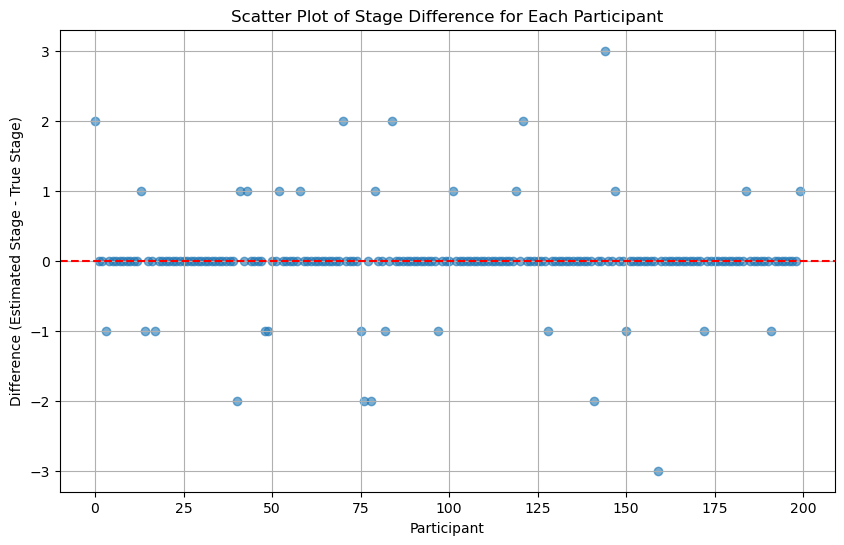
\includegraphics{estStages_files/figure-pdf/cell-11-output-1.png}

\section{Discussion}\label{discussion}

From the above result, we can see how challenging it is to accurately
estimate participant stages, \textbf{even if} we know exactly the
\(\theta\) and \(\phi\).

\begin{tcolorbox}[enhanced jigsaw, bottomrule=.15mm, colback=white, bottomtitle=1mm, titlerule=0mm, arc=.35mm, breakable, rightrule=.15mm, opacityback=0, leftrule=.75mm, opacitybacktitle=0.6, colframe=quarto-callout-tip-color-frame, coltitle=black, toptitle=1mm, colbacktitle=quarto-callout-tip-color!10!white, title=\textcolor{quarto-callout-tip-color}{\faLightbulb}\hspace{0.5em}{Tip}, left=2mm, toprule=.15mm]

What if we know only \(S\), but not \(\theta\) nor \(\phi\)?

The first step for us is to estimate \(\theta, \phi\) and then follow
the above procedures. To do that, refer back to
Chapter~\ref{sec-estimate-dist-params}.

\end{tcolorbox}

\bookmarksetup{startatroot}

\chapter{Estimate S}\label{estimate-s}

Now we come to the core part of our project: how can we estimate \(S\),
without knowing \(\theta, \phi, k_j\)?

Basically, this is the data we have:

\begin{Shaded}
\begin{Highlighting}[]
\ImportTok{import}\NormalTok{ pandas }\ImportTok{as}\NormalTok{ pd }
\NormalTok{output\_dir }\OperatorTok{=} \StringTok{\textquotesingle{}data\textquotesingle{}}
\NormalTok{df }\OperatorTok{=}\NormalTok{ pd.read\_csv(}\SpecialStringTok{f"}\SpecialCharTok{\{}\NormalTok{output\_dir}\SpecialCharTok{\}}\SpecialStringTok{/150|200\_3.csv"}\NormalTok{).drop(}
\NormalTok{    [}\StringTok{\textquotesingle{}k\_j\textquotesingle{}}\NormalTok{, }\StringTok{\textquotesingle{}S\_n\textquotesingle{}}\NormalTok{, }\StringTok{\textquotesingle{}affected\_or\_not\textquotesingle{}}\NormalTok{], axis }\OperatorTok{=} \DecValTok{1}\NormalTok{)}
\NormalTok{df.head()}
\end{Highlighting}
\end{Shaded}

\begin{longtable}[]{@{}lllll@{}}
\toprule\noalign{}
& participant & biomarker & measurement & diseased \\
\midrule\noalign{}
\endhead
\bottomrule\noalign{}
\endlastfoot
0 & 0 & HIP-FCI & 3.135981 & False \\
1 & 1 & HIP-FCI & 12.593704 & True \\
2 & 2 & HIP-FCI & 6.220776 & False \\
3 & 3 & HIP-FCI & 3.545100 & False \\
4 & 4 & HIP-FCI & 3.966541 & False \\
\end{longtable}

The main idea is this:

\begin{itemize}
\item
  We need to know \(\theta, \phi\) first before we can estimate
  likelihoods. To estimate \(\theta, \phi\), there are three approaches
  covered in Chapter~\ref{sec-estimate-dist-params}.
\item
  We try many different \(S\) and calculate its associated likelihood.
  We either accept or reject this \(S\) according to
  \href{https://en.wikipedia.org/wiki/Metropolis\%E2\%80\%93Hastings_algorithm}{Metropolis--Hastings
  algorithm}.
\end{itemize}

In the following, We will cover three different approaches to estimate
\(S\):

\begin{itemize}
\tightlist
\item
  Constrained K-Means
\item
  Conjugate Priors
\item
  Soft K-Means
\end{itemize}

\bookmarksetup{startatroot}

\chapter{\texorpdfstring{Estimate \(S\) with Constrained
K-Means}{Estimate S with Constrained K-Means}}\label{sec-estS-cop-kmeans}

The basic idea of using constrained K-Means to estimate \(S\) is:

\begin{itemize}
\tightlist
\item
  We first estimate distribution parameters using contrained K-Means,
  the exact procedure we covered in Section~\ref{sec-cop-kmeans}.
\item
  We use
  \href{https://en.wikipedia.org/wiki/Metropolis\%E2\%80\%93Hastings_algorithm}{Metropolis--Hastings
  algorithm} to accept or reject a proposed \(S\).
\end{itemize}

\section{Implementation}\label{implementation-1}

\begin{Shaded}
\begin{Highlighting}[]
\ImportTok{import}\NormalTok{ numpy }\ImportTok{as}\NormalTok{ np }
\ImportTok{import}\NormalTok{ utils }
\ImportTok{import}\NormalTok{ json }
\ImportTok{import}\NormalTok{ pandas }\ImportTok{as}\NormalTok{ pd }
\ImportTok{import}\NormalTok{ utils }
\ImportTok{from}\NormalTok{ scipy.stats }\ImportTok{import}\NormalTok{ kendalltau}
\ImportTok{import}\NormalTok{ sys}
\ImportTok{import}\NormalTok{ os}
\end{Highlighting}
\end{Shaded}

\begin{Shaded}
\begin{Highlighting}[]
\KeywordTok{def}\NormalTok{ calculate\_all\_participant\_ln\_likelihood(}
\NormalTok{        iteration,}
\NormalTok{        data\_we\_have,}
\NormalTok{        current\_order\_dict,}
\NormalTok{        n\_participants,}
\NormalTok{        non\_diseased\_participant\_ids,}
\NormalTok{        theta\_phi\_estimates,}
\NormalTok{        diseased\_stages,}
\NormalTok{):}
\NormalTok{    data }\OperatorTok{=}\NormalTok{ data\_we\_have.copy()}
\NormalTok{    data[}\StringTok{\textquotesingle{}S\_n\textquotesingle{}}\NormalTok{] }\OperatorTok{=}\NormalTok{ data.}\BuiltInTok{apply}\NormalTok{(}
        \KeywordTok{lambda}\NormalTok{ row: current\_order\_dict[row[}\StringTok{\textquotesingle{}biomarker\textquotesingle{}}\NormalTok{]], axis}\OperatorTok{=}\DecValTok{1}\NormalTok{)}
\NormalTok{    all\_participant\_ln\_likelihood }\OperatorTok{=} \DecValTok{0}

    \ControlFlowTok{for}\NormalTok{ p }\KeywordTok{in} \BuiltInTok{range}\NormalTok{(n\_participants):}
\NormalTok{        pdata }\OperatorTok{=}\NormalTok{ data[data.participant }\OperatorTok{==}\NormalTok{ p].reset\_index(drop}\OperatorTok{=}\VariableTok{True}\NormalTok{)}
        \ControlFlowTok{if}\NormalTok{ p }\KeywordTok{in}\NormalTok{ non\_diseased\_participant\_ids:}
\NormalTok{            this\_participant\_likelihood }\OperatorTok{=}\NormalTok{ utils.compute\_likelihood(}
\NormalTok{                pdata, k\_j}\OperatorTok{=}\DecValTok{0}\NormalTok{, theta\_phi}\OperatorTok{=}\NormalTok{theta\_phi\_estimates)}
\NormalTok{            this\_participant\_ln\_likelihood }\OperatorTok{=}\NormalTok{ np.log(}
\NormalTok{                this\_participant\_likelihood }\OperatorTok{+} \FloatTok{1e{-}10}\NormalTok{)}
        \ControlFlowTok{else}\NormalTok{:}
            \CommentTok{\# normalized\_stage\_likelihood\_dict = None}
            \CommentTok{\# initiaze stage\_likelihood}
\NormalTok{            stage\_likelihood\_dict }\OperatorTok{=}\NormalTok{ \{\}}
            \ControlFlowTok{for}\NormalTok{ k\_j }\KeywordTok{in}\NormalTok{ diseased\_stages:}
\NormalTok{                kj\_likelihood }\OperatorTok{=}\NormalTok{ utils.compute\_likelihood(}
\NormalTok{                    pdata, k\_j, theta\_phi\_estimates)}
                \CommentTok{\# update each stage likelihood for this participant}
\NormalTok{                stage\_likelihood\_dict[k\_j] }\OperatorTok{=}\NormalTok{ kj\_likelihood}
            \CommentTok{\# Add a small epsilon to avoid division by zero}
\NormalTok{            likelihood\_sum }\OperatorTok{=} \BuiltInTok{sum}\NormalTok{(stage\_likelihood\_dict.values())}

            \CommentTok{\# calculate weighted average}
\NormalTok{            this\_participant\_likelihood }\OperatorTok{=}\NormalTok{ np.mean(likelihood\_sum)}
\NormalTok{            this\_participant\_ln\_likelihood }\OperatorTok{=}\NormalTok{ np.log(}
\NormalTok{                this\_participant\_likelihood }\OperatorTok{+} \FloatTok{1e{-}10}\NormalTok{)}
\NormalTok{        all\_participant\_ln\_likelihood }\OperatorTok{+=}\NormalTok{ this\_participant\_ln\_likelihood}
    \ControlFlowTok{return}\NormalTok{ all\_participant\_ln\_likelihood}

\KeywordTok{def}\NormalTok{ metropolis\_hastings\_constrained\_kmeans(}
\NormalTok{    data\_we\_have,}
\NormalTok{    iterations,}
\NormalTok{    n\_shuffle,}
\NormalTok{):}
    \CommentTok{\textquotesingle{}\textquotesingle{}\textquotesingle{}Implement the metropolis{-}hastings algorithm using constrained kmeans}
\CommentTok{    Inputs: }
\CommentTok{        {-} data: data\_we\_have}
\CommentTok{        {-} iterations: number of iterations}
\CommentTok{        {-} log\_folder\_name: the folder where log files locate}

\CommentTok{    Outputs:}
\CommentTok{        {-} best\_order: a numpy array}
\CommentTok{        {-} best\_likelihood: a scalar }
\CommentTok{    \textquotesingle{}\textquotesingle{}\textquotesingle{}}
\NormalTok{    n\_participants }\OperatorTok{=} \BuiltInTok{len}\NormalTok{(data\_we\_have.participant.unique())}
\NormalTok{    biomarkers }\OperatorTok{=}\NormalTok{ data\_we\_have.biomarker.unique()}
\NormalTok{    n\_biomarkers }\OperatorTok{=} \BuiltInTok{len}\NormalTok{(biomarkers)}
\NormalTok{    n\_stages }\OperatorTok{=}\NormalTok{ n\_biomarkers }\OperatorTok{+} \DecValTok{1}
\NormalTok{    non\_diseased\_participant\_ids }\OperatorTok{=}\NormalTok{ data\_we\_have.loc[}
\NormalTok{        data\_we\_have.diseased }\OperatorTok{==} \VariableTok{False}\NormalTok{].participant.unique()}
\NormalTok{    diseased\_stages }\OperatorTok{=}\NormalTok{ np.arange(start}\OperatorTok{=}\DecValTok{1}\NormalTok{, stop}\OperatorTok{=}\NormalTok{n\_stages, step}\OperatorTok{=}\DecValTok{1}\NormalTok{)}
    \CommentTok{\# obtain the iniial theta and phi estimates}
\NormalTok{    theta\_phi\_estimates }\OperatorTok{=}\NormalTok{ utils.get\_theta\_phi\_estimates(}
\NormalTok{        data\_we\_have)}

    \CommentTok{\# initialize empty lists}
\NormalTok{    acceptance\_count }\OperatorTok{=} \DecValTok{0}
\NormalTok{    all\_current\_accepted\_order\_dicts }\OperatorTok{=}\NormalTok{ []}

\NormalTok{    current\_accepted\_order }\OperatorTok{=}\NormalTok{ np.random.permutation(np.arange(}\DecValTok{1}\NormalTok{, n\_stages))}
\NormalTok{    current\_accepted\_order\_dict }\OperatorTok{=} \BuiltInTok{dict}\NormalTok{(}\BuiltInTok{zip}\NormalTok{(biomarkers, current\_accepted\_order))}
\NormalTok{    current\_accepted\_likelihood }\OperatorTok{=} \OperatorTok{{-}}\NormalTok{np.inf}

    \ControlFlowTok{for}\NormalTok{ \_ }\KeywordTok{in} \BuiltInTok{range}\NormalTok{(iterations):}
        \CommentTok{\# in each iteration, we have updated current\_order\_dict and theta\_phi\_estimates}

\NormalTok{        new\_order }\OperatorTok{=}\NormalTok{ current\_accepted\_order.copy()}
\NormalTok{        utils.shuffle\_order(new\_order, n\_shuffle)}
\NormalTok{        current\_order\_dict }\OperatorTok{=} \BuiltInTok{dict}\NormalTok{(}\BuiltInTok{zip}\NormalTok{(biomarkers, new\_order))}
\NormalTok{        all\_participant\_ln\_likelihood }\OperatorTok{=}\NormalTok{ calculate\_all\_participant\_ln\_likelihood(}
\NormalTok{                \_,}
\NormalTok{                data\_we\_have,}
\NormalTok{                current\_order\_dict,}
\NormalTok{                n\_participants,}
\NormalTok{                non\_diseased\_participant\_ids,}
\NormalTok{                theta\_phi\_estimates,}
\NormalTok{                diseased\_stages,}
\NormalTok{            )}


        \CommentTok{\# Log{-}Sum{-}Exp Trick}
\NormalTok{        max\_likelihood }\OperatorTok{=} \BuiltInTok{max}\NormalTok{(all\_participant\_ln\_likelihood,}
\NormalTok{                             current\_accepted\_likelihood)}
\NormalTok{        prob\_of\_accepting\_new\_order }\OperatorTok{=}\NormalTok{ np.exp(}
\NormalTok{            (all\_participant\_ln\_likelihood }\OperatorTok{{-}}\NormalTok{ max\_likelihood) }\OperatorTok{{-}}
\NormalTok{            (current\_accepted\_likelihood }\OperatorTok{{-}}\NormalTok{ max\_likelihood)}
\NormalTok{        )}

        \CommentTok{\# prob\_of\_accepting\_new\_order = np.exp(}
        \CommentTok{\#     all\_participant\_ln\_likelihood {-} current\_accepted\_likelihood)}

        \CommentTok{\# np.exp(a)/np.exp(b) = np.exp(a {-} b)}
        \CommentTok{\# if a \textgreater{} b, then np.exp(a {-} b) \textgreater{} 1}

        \CommentTok{\# it will definitly update at the first iteration}
        \ControlFlowTok{if}\NormalTok{ np.random.rand() }\OperatorTok{\textless{}}\NormalTok{ prob\_of\_accepting\_new\_order:}
\NormalTok{            acceptance\_count }\OperatorTok{+=} \DecValTok{1}
\NormalTok{            current\_accepted\_order }\OperatorTok{=}\NormalTok{ new\_order}
\NormalTok{            current\_accepted\_likelihood }\OperatorTok{=}\NormalTok{ all\_participant\_ln\_likelihood}
\NormalTok{            current\_accepted\_order\_dict }\OperatorTok{=}\NormalTok{ current\_order\_dict}

\NormalTok{        acceptance\_ratio }\OperatorTok{=}\NormalTok{ acceptance\_count}\OperatorTok{*}\DecValTok{100}\OperatorTok{/}\NormalTok{(\_}\OperatorTok{+}\DecValTok{1}\NormalTok{)}
\NormalTok{        all\_current\_accepted\_order\_dicts.append(current\_accepted\_order\_dict)}

        \ControlFlowTok{if}\NormalTok{ (\_}\OperatorTok{+}\DecValTok{1}\NormalTok{) }\OperatorTok{\%} \DecValTok{10} \OperatorTok{==} \DecValTok{0}\NormalTok{:}
\NormalTok{            formatted\_string }\OperatorTok{=}\NormalTok{ (}
                \SpecialStringTok{f"iteration }\SpecialCharTok{\{}\NormalTok{\_ }\OperatorTok{+} \DecValTok{1}\SpecialCharTok{\}}\SpecialStringTok{ done, "}
                \SpecialStringTok{f"current accepted likelihood: }\SpecialCharTok{\{}\NormalTok{current\_accepted\_likelihood}\SpecialCharTok{\}}\SpecialStringTok{, "}
                \SpecialStringTok{f"current acceptance ratio is }\SpecialCharTok{\{}\NormalTok{acceptance\_ratio}\SpecialCharTok{:.2f\}}\SpecialStringTok{ \%, "}
                \SpecialStringTok{f"current accepted order is }\SpecialCharTok{\{}\NormalTok{current\_accepted\_order\_dict}\SpecialCharTok{.}\NormalTok{values()}\SpecialCharTok{\}}\SpecialStringTok{, "}
\NormalTok{            )}
            \BuiltInTok{print}\NormalTok{(formatted\_string)}

    \CommentTok{\# print("done!")}
    \ControlFlowTok{return}\NormalTok{ all\_current\_accepted\_order\_dicts}
\end{Highlighting}
\end{Shaded}

\begin{Shaded}
\begin{Highlighting}[]
\NormalTok{n\_shuffle }\OperatorTok{=} \DecValTok{2}
\NormalTok{iterations }\OperatorTok{=} \DecValTok{10}
\NormalTok{burn\_in }\OperatorTok{=} \DecValTok{2}
\NormalTok{thining }\OperatorTok{=} \DecValTok{2}

\NormalTok{base\_dir }\OperatorTok{=}\NormalTok{ os.getcwd()}
\BuiltInTok{print}\NormalTok{(}\SpecialStringTok{f"Current working directory: }\SpecialCharTok{\{}\NormalTok{base\_dir}\SpecialCharTok{\}}\SpecialStringTok{"}\NormalTok{)}
\NormalTok{data\_dir }\OperatorTok{=}\NormalTok{ os.path.join(base\_dir, }\StringTok{"data"}\NormalTok{)}

\NormalTok{cop\_kmeans\_dir }\OperatorTok{=}\NormalTok{ os.path.join(base\_dir, }\StringTok{\textquotesingle{}cop\_kmeans\textquotesingle{}}\NormalTok{)}
\NormalTok{temp\_results\_dir }\OperatorTok{=}\NormalTok{ os.path.join(cop\_kmeans\_dir, }\StringTok{"temp\_json\_results"}\NormalTok{)}
\NormalTok{img\_dir }\OperatorTok{=}\NormalTok{ os.path.join(cop\_kmeans\_dir, }\StringTok{\textquotesingle{}img\textquotesingle{}}\NormalTok{)}
\NormalTok{results\_file }\OperatorTok{=}\NormalTok{ os.path.join(cop\_kmeans\_dir, }\StringTok{"results.json"}\NormalTok{)}

\NormalTok{os.makedirs(cop\_kmeans\_dir, exist\_ok}\OperatorTok{=}\VariableTok{True}\NormalTok{)}
\NormalTok{os.makedirs(temp\_results\_dir, exist\_ok}\OperatorTok{=}\VariableTok{True}\NormalTok{)}
\NormalTok{os.makedirs(img\_dir, exist\_ok}\OperatorTok{=}\VariableTok{True}\NormalTok{)}

\BuiltInTok{print}\NormalTok{(}\SpecialStringTok{f"Data directory: }\SpecialCharTok{\{}\NormalTok{data\_dir}\SpecialCharTok{\}}\SpecialStringTok{"}\NormalTok{)}
\BuiltInTok{print}\NormalTok{(}\SpecialStringTok{f"Temp results directory: }\SpecialCharTok{\{}\NormalTok{temp\_results\_dir}\SpecialCharTok{\}}\SpecialStringTok{"}\NormalTok{)}
\BuiltInTok{print}\NormalTok{(}\SpecialStringTok{f"Image directory: }\SpecialCharTok{\{}\NormalTok{img\_dir}\SpecialCharTok{\}}\SpecialStringTok{"}\NormalTok{)}

\ControlFlowTok{if} \VariableTok{\_\_name\_\_} \OperatorTok{==} \StringTok{"\_\_main\_\_"}\NormalTok{:}

    \CommentTok{\# Read parameters from command line arguments}
\NormalTok{    j }\OperatorTok{=} \DecValTok{200}
\NormalTok{    r }\OperatorTok{=} \FloatTok{0.75}
\NormalTok{    m }\OperatorTok{=} \DecValTok{3}

    \BuiltInTok{print}\NormalTok{(}\SpecialStringTok{f"Processing with j=}\SpecialCharTok{\{}\NormalTok{j}\SpecialCharTok{\}}\SpecialStringTok{, r=}\SpecialCharTok{\{}\NormalTok{r}\SpecialCharTok{\}}\SpecialStringTok{, m=}\SpecialCharTok{\{}\NormalTok{m}\SpecialCharTok{\}}\SpecialStringTok{"}\NormalTok{)}

\NormalTok{    combstr }\OperatorTok{=} \SpecialStringTok{f"}\SpecialCharTok{\{}\BuiltInTok{int}\NormalTok{(j}\OperatorTok{*}\NormalTok{r)}\SpecialCharTok{\}}\SpecialStringTok{|}\SpecialCharTok{\{}\NormalTok{j}\SpecialCharTok{\}}\SpecialStringTok{"}
\NormalTok{    heatmap\_folder }\OperatorTok{=}\NormalTok{ img\_dir}
    
\NormalTok{    filename }\OperatorTok{=} \SpecialStringTok{f"}\SpecialCharTok{\{}\NormalTok{combstr}\SpecialCharTok{\}}\SpecialStringTok{\_}\SpecialCharTok{\{}\NormalTok{m}\SpecialCharTok{\}}\SpecialStringTok{"}
\NormalTok{    data\_file }\OperatorTok{=} \SpecialStringTok{f"}\SpecialCharTok{\{}\NormalTok{data\_dir}\SpecialCharTok{\}}\SpecialStringTok{/}\SpecialCharTok{\{}\NormalTok{filename}\SpecialCharTok{\}}\SpecialStringTok{.csv"}
\NormalTok{    data\_we\_have }\OperatorTok{=}\NormalTok{ pd.read\_csv(data\_file)}
\NormalTok{    n\_biomarkers }\OperatorTok{=} \BuiltInTok{len}\NormalTok{(data\_we\_have.biomarker.unique())}

    \ControlFlowTok{if} \KeywordTok{not}\NormalTok{ os.path.exists(data\_file):}
        \BuiltInTok{print}\NormalTok{(}\SpecialStringTok{f"Data file not found: }\SpecialCharTok{\{}\NormalTok{data\_file}\SpecialCharTok{\}}\SpecialStringTok{"}\NormalTok{)}
\NormalTok{        sys.exit(}\DecValTok{1}\NormalTok{)  }\CommentTok{\# Exit early if the file doesn\textquotesingle{}t exist}
    \ControlFlowTok{else}\NormalTok{:}
        \BuiltInTok{print}\NormalTok{(}\SpecialStringTok{f"Data file found: }\SpecialCharTok{\{}\NormalTok{data\_file}\SpecialCharTok{\}}\SpecialStringTok{"}\NormalTok{)}

    \CommentTok{\# Define the temporary result file}
\NormalTok{    temp\_result\_file }\OperatorTok{=}\NormalTok{ os.path.join(temp\_results\_dir, }\SpecialStringTok{f"temp\_results\_}\SpecialCharTok{\{}\NormalTok{j}\SpecialCharTok{\}}\SpecialStringTok{\_}\SpecialCharTok{\{}\NormalTok{r}\SpecialCharTok{\}}\SpecialStringTok{\_}\SpecialCharTok{\{}\NormalTok{m}\SpecialCharTok{\}}\SpecialStringTok{.json"}\NormalTok{)}
    
\NormalTok{    dic }\OperatorTok{=}\NormalTok{ \{\}}

    \ControlFlowTok{if}\NormalTok{ combstr }\KeywordTok{not} \KeywordTok{in}\NormalTok{ dic:}
\NormalTok{        dic[combstr] }\OperatorTok{=}\NormalTok{ []}

\NormalTok{    accepted\_order\_dicts }\OperatorTok{=}\NormalTok{ metropolis\_hastings\_constrained\_kmeans(}
\NormalTok{        data\_we\_have,}
\NormalTok{        iterations,}
\NormalTok{        n\_shuffle,}
\NormalTok{    )}

\NormalTok{    utils.save\_heatmap(}
\NormalTok{        accepted\_order\_dicts,}
\NormalTok{        burn\_in, }
\NormalTok{        thining, }
\NormalTok{        folder\_name}\OperatorTok{=}\NormalTok{heatmap\_folder,}
\NormalTok{        file\_name}\OperatorTok{=}\SpecialStringTok{f"}\SpecialCharTok{\{}\NormalTok{filename}\SpecialCharTok{\}}\SpecialStringTok{"}\NormalTok{, }
\NormalTok{        title}\OperatorTok{=}\SpecialStringTok{f\textquotesingle{}heatmap of }\SpecialCharTok{\{}\NormalTok{filename}\SpecialCharTok{\}}\SpecialStringTok{\textquotesingle{}}\NormalTok{)}
    
\NormalTok{    most\_likely\_order\_dic }\OperatorTok{=}\NormalTok{ utils.obtain\_most\_likely\_order\_dic(}
\NormalTok{        accepted\_order\_dicts, burn\_in, thining)}
\NormalTok{    most\_likely\_order }\OperatorTok{=} \BuiltInTok{list}\NormalTok{(most\_likely\_order\_dic.values())}
\NormalTok{    tau, p\_value }\OperatorTok{=}\NormalTok{ kendalltau(most\_likely\_order, }\BuiltInTok{range}\NormalTok{(}\DecValTok{1}\NormalTok{, n\_biomarkers }\OperatorTok{+} \DecValTok{1}\NormalTok{))}
    
\NormalTok{    dic[combstr].append(tau)}
    
    \CommentTok{\# Write the results to a unique temporary file inside the temp folder}
    \ControlFlowTok{with} \BuiltInTok{open}\NormalTok{(temp\_result\_file, }\StringTok{"w"}\NormalTok{) }\ImportTok{as} \BuiltInTok{file}\NormalTok{:}
\NormalTok{        json.dump(dic, }\BuiltInTok{file}\NormalTok{, indent}\OperatorTok{=}\DecValTok{4}\NormalTok{)}
    \BuiltInTok{print}\NormalTok{(}\SpecialStringTok{f"}\SpecialCharTok{\{}\NormalTok{filename}\SpecialCharTok{\}}\SpecialStringTok{ is done! Results written to }\SpecialCharTok{\{}\NormalTok{temp\_result\_file}\SpecialCharTok{\}}\SpecialStringTok{"}\NormalTok{)}
\end{Highlighting}
\end{Shaded}

\begin{verbatim}
Current working directory: /Users/hongtaoh/Desktop/github/ebmBook
Data directory: /Users/hongtaoh/Desktop/github/ebmBook/data
Temp results directory: /Users/hongtaoh/Desktop/github/ebmBook/cop_kmeans/temp_json_results
Image directory: /Users/hongtaoh/Desktop/github/ebmBook/cop_kmeans/img
Processing with j=200, r=0.75, m=3
Data file found: /Users/hongtaoh/Desktop/github/ebmBook/data/150|200_3.csv
iteration 10 done, current accepted likelihood: -4389.297238189531, current acceptance ratio is 80.00 %, current accepted order is dict_values([1, 9, 6, 8, 3, 2, 10, 7, 5, 4]), 
150|200_3 is done! Results written to /Users/hongtaoh/Desktop/github/ebmBook/cop_kmeans/temp_json_results/temp_results_200_0.75_3.json
\end{verbatim}

\section{Result}\label{result-1}

We plot the resulting \(S\) probalistically using a heatmap. We also
quantify the difference between our result with the real \(S\) using
\href{https://en.wikipedia.org/wiki/Kendall_rank_correlation_coefficient}{Kendall's
Tau}. It ranges from \(-1\) (completely different) to \(1\) (exactly the
same). \(0\) indicate complete randomness.

\begin{figure}

\centering{

\includegraphics{cop_kmeans/img/150\%7C200_3.png}

}

\caption{\label{fig-cop-kmeans-result}Result of Constrained K-Means}

\end{figure}%

\begin{Shaded}
\begin{Highlighting}[]
\NormalTok{dic}
\end{Highlighting}
\end{Shaded}

\begin{verbatim}
{'150|200': [-0.022222222222222223]}
\end{verbatim}

\bookmarksetup{startatroot}

\chapter{\texorpdfstring{Estimate \(S\) with Soft
K-Means}{Estimate S with Soft K-Means}}\label{sec-estS-soft-kmeans}

The basic idea of using Soft K-Means to estimate \(S\) is:

\begin{itemize}
\tightlist
\item
  We first estimate distribution parameters using contrained K-Means,
  the exact procedure we covered in Section~\ref{sec-cop-kmeans}.
\item
  In each iteration, we use Soft Kmeans algorithm to update
  \(\theta, \phi\) (refer to Section~\ref{sec-soft-kmeans}) and use
  \href{https://en.wikipedia.org/wiki/Metropolis\%E2\%80\%93Hastings_algorithm}{Metropolis--Hastings
  algorithm} to accept or reject a proposed \(S\).
\end{itemize}

\section{Implementation}\label{implementation-2}

\begin{Shaded}
\begin{Highlighting}[]
\ImportTok{import}\NormalTok{ numpy }\ImportTok{as}\NormalTok{ np }
\ImportTok{import}\NormalTok{ utils }
\ImportTok{import}\NormalTok{ json }
\ImportTok{import}\NormalTok{ pandas }\ImportTok{as}\NormalTok{ pd }
\ImportTok{import}\NormalTok{ utils }
\ImportTok{from}\NormalTok{ scipy.stats }\ImportTok{import}\NormalTok{ kendalltau}
\ImportTok{import}\NormalTok{ sys}
\ImportTok{import}\NormalTok{ os}
\ImportTok{import}\NormalTok{ math }
\end{Highlighting}
\end{Shaded}

\begin{Shaded}
\begin{Highlighting}[]
\KeywordTok{def}\NormalTok{ calculate\_soft\_kmeans\_for\_biomarker(}
\NormalTok{        data,}
\NormalTok{        biomarker,}
\NormalTok{        order\_dict,}
\NormalTok{        n\_participants,}
\NormalTok{        non\_diseased\_participants,}
\NormalTok{        hashmap\_of\_normalized\_stage\_likelihood\_dicts,}
\NormalTok{        diseased\_stages,}
\NormalTok{        seed}\OperatorTok{=}\VariableTok{None}
\NormalTok{):}
    \CommentTok{"""}
\CommentTok{    Calculate mean and std for both the affected and non{-}affected clusters for a single biomarker.}

\CommentTok{    Parameters:}
\CommentTok{        data (pd.DataFrame): The data containing measurements.}
\CommentTok{        biomarker (str): The biomarker to process.}
\CommentTok{        order\_dict (dict): Dictionary mapping biomarkers to their order.}
\CommentTok{        n\_participants (int): Number of participants in the study.}
\CommentTok{        non\_diseased\_participants (list): List of non{-}diseased participants.}
\CommentTok{        hashmap\_of\_normalized\_stage\_likelihood\_dicts (dict): Hash map of }
\CommentTok{            dictionaries containing stage likelihoods for each participant.}
\CommentTok{        diseased\_stages (list): List of diseased stages.}
\CommentTok{        seed (int, optional): Random seed for reproducibility.}

\CommentTok{    Returns:}
\CommentTok{        tuple: Means and standard deviations for affected and non{-}affected clusters.}
\CommentTok{    """}
    \ControlFlowTok{if}\NormalTok{ seed }\KeywordTok{is} \KeywordTok{not} \VariableTok{None}\NormalTok{:}
        \CommentTok{\# Set the seed for numpy\textquotesingle{}s random number generator}
\NormalTok{        rng }\OperatorTok{=}\NormalTok{ np.random.default\_rng(seed)}
    \ControlFlowTok{else}\NormalTok{:}
\NormalTok{        rng }\OperatorTok{=}\NormalTok{ np.random }

    \CommentTok{\# DataFrame for this biomarker}
\NormalTok{    biomarker\_df }\OperatorTok{=}\NormalTok{ data[}
\NormalTok{        data[}\StringTok{\textquotesingle{}biomarker\textquotesingle{}}\NormalTok{] }\OperatorTok{==}\NormalTok{ biomarker].reset\_index(}
\NormalTok{            drop}\OperatorTok{=}\VariableTok{True}\NormalTok{).sort\_values(}
\NormalTok{                by }\OperatorTok{=} \StringTok{\textquotesingle{}participant\textquotesingle{}}\NormalTok{, ascending }\OperatorTok{=} \VariableTok{True}\NormalTok{)}
    \CommentTok{\# Extract measurements}
\NormalTok{    measurements }\OperatorTok{=}\NormalTok{ np.array(biomarker\_df[}\StringTok{\textquotesingle{}measurement\textquotesingle{}}\NormalTok{])}

\NormalTok{    this\_biomarker\_order }\OperatorTok{=}\NormalTok{ order\_dict[biomarker]}

\NormalTok{    affected\_cluster }\OperatorTok{=}\NormalTok{ []}
\NormalTok{    non\_affected\_cluster }\OperatorTok{=}\NormalTok{ []}

    \ControlFlowTok{for}\NormalTok{ p }\KeywordTok{in} \BuiltInTok{range}\NormalTok{(n\_participants):}
        \ControlFlowTok{if}\NormalTok{ p }\KeywordTok{in}\NormalTok{ non\_diseased\_participants:}
\NormalTok{            non\_affected\_cluster.append(measurements[p])}
        \ControlFlowTok{else}\NormalTok{:}
            \ControlFlowTok{if}\NormalTok{ this\_biomarker\_order }\OperatorTok{==} \DecValTok{1}\NormalTok{:}
\NormalTok{                affected\_cluster.append(measurements[p])}
            \ControlFlowTok{else}\NormalTok{:}
\NormalTok{                normalized\_stage\_likelihood\_dict }\OperatorTok{=}\NormalTok{ hashmap\_of\_normalized\_stage\_likelihood\_dicts[}
\NormalTok{                    p]}
                \CommentTok{\# Calculate probabilities for affected and non{-}affected states}
\NormalTok{                affected\_prob }\OperatorTok{=} \BuiltInTok{sum}\NormalTok{(}
\NormalTok{                    normalized\_stage\_likelihood\_dict[s] }\ControlFlowTok{for}\NormalTok{ s }\KeywordTok{in}\NormalTok{ diseased\_stages }\ControlFlowTok{if}\NormalTok{ s }\OperatorTok{\textgreater{}=}\NormalTok{ this\_biomarker\_order}
\NormalTok{                )}
\NormalTok{                non\_affected\_prob }\OperatorTok{=} \BuiltInTok{sum}\NormalTok{(}
\NormalTok{                    normalized\_stage\_likelihood\_dict[s] }\ControlFlowTok{for}\NormalTok{ s }\KeywordTok{in}\NormalTok{ diseased\_stages }\ControlFlowTok{if}\NormalTok{ s }\OperatorTok{\textless{}}\NormalTok{ this\_biomarker\_order}
\NormalTok{                )}
                \ControlFlowTok{if}\NormalTok{ affected\_prob }\OperatorTok{\textgreater{}}\NormalTok{ non\_affected\_prob:}
\NormalTok{                    affected\_cluster.append(measurements[p])}
                \ControlFlowTok{elif}\NormalTok{ affected\_prob }\OperatorTok{\textless{}}\NormalTok{ non\_affected\_prob:}
\NormalTok{                    non\_affected\_cluster.append(measurements[p])}
                \ControlFlowTok{else}\NormalTok{:}
                    \CommentTok{\# Assign to either cluster randomly if probabilities are equal}
                    \ControlFlowTok{if}\NormalTok{ rng.random() }\OperatorTok{\textgreater{}} \FloatTok{0.5}\NormalTok{:}
\NormalTok{                        affected\_cluster.append(measurements[p])}
                    \ControlFlowTok{else}\NormalTok{:}
\NormalTok{                        non\_affected\_cluster.append(measurements[p])}

    \CommentTok{\# Compute means and standard deviations}
\NormalTok{    theta\_mean }\OperatorTok{=}\NormalTok{ np.mean(affected\_cluster) }\ControlFlowTok{if}\NormalTok{ affected\_cluster }\ControlFlowTok{else}\NormalTok{ np.nan}
\NormalTok{    theta\_std }\OperatorTok{=}\NormalTok{ np.std(affected\_cluster) }\ControlFlowTok{if}\NormalTok{ affected\_cluster }\ControlFlowTok{else}\NormalTok{ np.nan}
\NormalTok{    phi\_mean }\OperatorTok{=}\NormalTok{ np.mean(}
\NormalTok{        non\_affected\_cluster) }\ControlFlowTok{if}\NormalTok{ non\_affected\_cluster }\ControlFlowTok{else}\NormalTok{ np.nan}
\NormalTok{    phi\_std }\OperatorTok{=}\NormalTok{ np.std(non\_affected\_cluster) }\ControlFlowTok{if}\NormalTok{ non\_affected\_cluster }\ControlFlowTok{else}\NormalTok{ np.nan}
    \ControlFlowTok{return}\NormalTok{ theta\_mean, theta\_std, phi\_mean, phi\_std}

\KeywordTok{def}\NormalTok{ soft\_kmeans\_theta\_phi\_estimates(}
\NormalTok{        iteration,}
\NormalTok{        prior\_theta\_phi\_estimates,}
\NormalTok{        data\_we\_have,}
\NormalTok{        biomarkers,}
\NormalTok{        order\_dict,}
\NormalTok{        n\_participants,}
\NormalTok{        non\_diseased\_participants,}
\NormalTok{        hashmap\_of\_normalized\_stage\_likelihood\_dicts,}
\NormalTok{        diseased\_stages,}
\NormalTok{        seed}\OperatorTok{=}\VariableTok{None}\NormalTok{):}
    \CommentTok{"""}
\CommentTok{    Get the DataFrame of theta and phi using the soft K{-}means algorithm for all biomarkers.}

\CommentTok{    Parameters:}
\CommentTok{        data\_we\_have (pd.DataFrame): DataFrame containing the data.}
\CommentTok{        biomarkers (list): List of biomarkers in string.}
\CommentTok{        order\_dict (dict): Dictionary mapping biomarkers to their order.}
\CommentTok{        n\_participants (int): Number of participants in the study.}
\CommentTok{        non\_diseased\_participants (list): List of non{-}diseased participants.}
\CommentTok{        hashmap\_of\_normalized\_stage\_likelihood\_dicts (dict): Hash map of dictionaries containing stage likelihoods for each participant.}
\CommentTok{        diseased\_stages (list): List of diseased stages.}
\CommentTok{        seed (int, optional): Random seed for reproducibility.}

\CommentTok{    Returns:}
\CommentTok{        a dictionary containing the means and standard deviations for theta and phi for each biomarker.}
\CommentTok{    """}
    \CommentTok{\# List of dicts to store the estimates}
    \CommentTok{\# In each dic, key is biomarker, and values are theta and phi params}
\NormalTok{    hashmap\_of\_means\_stds\_estimate\_dicts }\OperatorTok{=}\NormalTok{ \{\}}
    \ControlFlowTok{for}\NormalTok{ biomarker }\KeywordTok{in}\NormalTok{ biomarkers:}
\NormalTok{        dic }\OperatorTok{=}\NormalTok{ \{}\StringTok{\textquotesingle{}biomarker\textquotesingle{}}\NormalTok{: biomarker\}}
\NormalTok{        prior\_theta\_phi\_estimates\_biomarker }\OperatorTok{=}\NormalTok{ prior\_theta\_phi\_estimates[biomarker]}
\NormalTok{        theta\_mean, theta\_std, phi\_mean, phi\_std }\OperatorTok{=}\NormalTok{ calculate\_soft\_kmeans\_for\_biomarker(}
\NormalTok{            data\_we\_have,}
\NormalTok{            biomarker,}
\NormalTok{            order\_dict,}
\NormalTok{            n\_participants,}
\NormalTok{            non\_diseased\_participants,}
\NormalTok{            hashmap\_of\_normalized\_stage\_likelihood\_dicts,}
\NormalTok{            diseased\_stages,}
\NormalTok{            seed}
\NormalTok{        )}
        \ControlFlowTok{if}\NormalTok{ theta\_std }\OperatorTok{==} \DecValTok{0} \KeywordTok{or}\NormalTok{ math.isnan(theta\_std):}
\NormalTok{            theta\_mean }\OperatorTok{=}\NormalTok{ prior\_theta\_phi\_estimates\_biomarker[}\StringTok{\textquotesingle{}theta\_mean\textquotesingle{}}\NormalTok{]}
\NormalTok{            theta\_std }\OperatorTok{=}\NormalTok{ prior\_theta\_phi\_estimates\_biomarker[}\StringTok{\textquotesingle{}theta\_std\textquotesingle{}}\NormalTok{]}
        \ControlFlowTok{if}\NormalTok{ phi\_std }\OperatorTok{==} \DecValTok{0} \KeywordTok{or}\NormalTok{ math.isnan(phi\_std):}
\NormalTok{            phi\_mean }\OperatorTok{=}\NormalTok{ prior\_theta\_phi\_estimates\_biomarker[}\StringTok{\textquotesingle{}phi\_mean\textquotesingle{}}\NormalTok{]}
\NormalTok{            phi\_std }\OperatorTok{=}\NormalTok{ prior\_theta\_phi\_estimates\_biomarker[}\StringTok{\textquotesingle{}phi\_std\textquotesingle{}}\NormalTok{]}
\NormalTok{        dic[}\StringTok{\textquotesingle{}theta\_mean\textquotesingle{}}\NormalTok{] }\OperatorTok{=}\NormalTok{ theta\_mean}
\NormalTok{        dic[}\StringTok{\textquotesingle{}theta\_std\textquotesingle{}}\NormalTok{] }\OperatorTok{=}\NormalTok{ theta\_std}
\NormalTok{        dic[}\StringTok{\textquotesingle{}phi\_mean\textquotesingle{}}\NormalTok{] }\OperatorTok{=}\NormalTok{ phi\_mean}
\NormalTok{        dic[}\StringTok{\textquotesingle{}phi\_std\textquotesingle{}}\NormalTok{] }\OperatorTok{=}\NormalTok{ phi\_std}
\NormalTok{        hashmap\_of\_means\_stds\_estimate\_dicts[biomarker] }\OperatorTok{=}\NormalTok{ dic}
    \ControlFlowTok{return}\NormalTok{ hashmap\_of\_means\_stds\_estimate\_dicts}

\KeywordTok{def}\NormalTok{ calculate\_all\_participant\_ln\_likelihood\_and\_update\_hashmap(}
\NormalTok{        iteration,}
\NormalTok{        data\_we\_have,}
\NormalTok{        current\_order\_dict,}
\NormalTok{        n\_participants,}
\NormalTok{        non\_diseased\_participant\_ids,}
\NormalTok{        theta\_phi\_estimates,}
\NormalTok{        diseased\_stages,}
\NormalTok{):}
\NormalTok{    data }\OperatorTok{=}\NormalTok{ data\_we\_have.copy()}
\NormalTok{    data[}\StringTok{\textquotesingle{}S\_n\textquotesingle{}}\NormalTok{] }\OperatorTok{=}\NormalTok{ data.}\BuiltInTok{apply}\NormalTok{(}
        \KeywordTok{lambda}\NormalTok{ row: current\_order\_dict[row[}\StringTok{\textquotesingle{}biomarker\textquotesingle{}}\NormalTok{]], axis}\OperatorTok{=}\DecValTok{1}\NormalTok{)}
\NormalTok{    all\_participant\_ln\_likelihood }\OperatorTok{=} \DecValTok{0}
    \CommentTok{\# key is participant id}
    \CommentTok{\# value is normalized\_stage\_likelihood\_dict}
\NormalTok{    hashmap\_of\_normalized\_stage\_likelihood\_dicts }\OperatorTok{=}\NormalTok{ \{\}}
    \ControlFlowTok{for}\NormalTok{ p }\KeywordTok{in} \BuiltInTok{range}\NormalTok{(n\_participants):}
\NormalTok{        pdata }\OperatorTok{=}\NormalTok{ data[data.participant }\OperatorTok{==}\NormalTok{ p].reset\_index(drop}\OperatorTok{=}\VariableTok{True}\NormalTok{)}
        \ControlFlowTok{if}\NormalTok{ p }\KeywordTok{in}\NormalTok{ non\_diseased\_participant\_ids:}
\NormalTok{            this\_participant\_likelihood }\OperatorTok{=}\NormalTok{ utils.compute\_likelihood(}
\NormalTok{                pdata, k\_j}\OperatorTok{=}\DecValTok{0}\NormalTok{, theta\_phi}\OperatorTok{=}\NormalTok{theta\_phi\_estimates)}
\NormalTok{            this\_participant\_ln\_likelihood }\OperatorTok{=}\NormalTok{ np.log(}
\NormalTok{                this\_participant\_likelihood }\OperatorTok{+} \FloatTok{1e{-}10}\NormalTok{)}
        \ControlFlowTok{else}\NormalTok{:}
            \CommentTok{\# normalized\_stage\_likelihood\_dict = None}
            \CommentTok{\# initiaze stage\_likelihood}
\NormalTok{            stage\_likelihood\_dict }\OperatorTok{=}\NormalTok{ \{\}}
            \ControlFlowTok{for}\NormalTok{ k\_j }\KeywordTok{in}\NormalTok{ diseased\_stages:}
\NormalTok{                kj\_likelihood }\OperatorTok{=}\NormalTok{ utils.compute\_likelihood(}
\NormalTok{                    pdata, k\_j, theta\_phi\_estimates)}
                \CommentTok{\# update each stage likelihood for this participant}
\NormalTok{                stage\_likelihood\_dict[k\_j] }\OperatorTok{=}\NormalTok{ kj\_likelihood}
            \CommentTok{\# Add a small epsilon to avoid division by zero}
\NormalTok{            likelihood\_sum }\OperatorTok{=} \BuiltInTok{sum}\NormalTok{(stage\_likelihood\_dict.values())}
\NormalTok{            epsilon }\OperatorTok{=} \FloatTok{1e{-}10}
            \ControlFlowTok{if}\NormalTok{ likelihood\_sum }\OperatorTok{==} \DecValTok{0}\NormalTok{:}
                \CommentTok{\# print("Invalid likelihood\_sum: zero encountered.")}
\NormalTok{                likelihood\_sum }\OperatorTok{=}\NormalTok{ epsilon  }\CommentTok{\# Handle the case accordingly}
\NormalTok{            normalized\_stage\_likelihood }\OperatorTok{=}\NormalTok{ [}
\NormalTok{                l}\OperatorTok{/}\NormalTok{likelihood\_sum }\ControlFlowTok{for}\NormalTok{ l }\KeywordTok{in}\NormalTok{ stage\_likelihood\_dict.values()]}
\NormalTok{            normalized\_stage\_likelihood\_dict }\OperatorTok{=} \BuiltInTok{dict}\NormalTok{(}
                \BuiltInTok{zip}\NormalTok{(diseased\_stages, normalized\_stage\_likelihood))}
\NormalTok{            hashmap\_of\_normalized\_stage\_likelihood\_dicts[p] }\OperatorTok{=}\NormalTok{ normalized\_stage\_likelihood\_dict}

            \CommentTok{\# calculate weighted average}
\NormalTok{            this\_participant\_likelihood }\OperatorTok{=}\NormalTok{ np.mean(likelihood\_sum)}
\NormalTok{            this\_participant\_ln\_likelihood }\OperatorTok{=}\NormalTok{ np.log(}
\NormalTok{                this\_participant\_likelihood)}
\NormalTok{        all\_participant\_ln\_likelihood }\OperatorTok{+=}\NormalTok{ this\_participant\_ln\_likelihood}
    \ControlFlowTok{return}\NormalTok{ all\_participant\_ln\_likelihood, hashmap\_of\_normalized\_stage\_likelihood\_dicts}


\KeywordTok{def}\NormalTok{ metropolis\_hastings\_soft\_kmeans(}
\NormalTok{    data\_we\_have,}
\NormalTok{    iterations,}
\NormalTok{    n\_shuffle,}
\NormalTok{):}
    \CommentTok{\textquotesingle{}\textquotesingle{}\textquotesingle{}Implement the metropolis{-}hastings algorithm using soft kmeans}
\CommentTok{    Inputs: }
\CommentTok{        {-} data: data\_we\_have}
\CommentTok{        {-} iterations: number of iterations}
\CommentTok{        {-} log\_folder\_name: the folder where log files locate}

\CommentTok{    Outputs:}
\CommentTok{        {-} best\_order: a numpy array}
\CommentTok{        {-} best\_likelihood: a scalar }
\CommentTok{    \textquotesingle{}\textquotesingle{}\textquotesingle{}}
\NormalTok{    n\_participants }\OperatorTok{=} \BuiltInTok{len}\NormalTok{(data\_we\_have.participant.unique())}
\NormalTok{    biomarkers }\OperatorTok{=}\NormalTok{ data\_we\_have.biomarker.unique()}
\NormalTok{    n\_biomarkers }\OperatorTok{=} \BuiltInTok{len}\NormalTok{(biomarkers)}
\NormalTok{    n\_stages }\OperatorTok{=}\NormalTok{ n\_biomarkers }\OperatorTok{+} \DecValTok{1}
\NormalTok{    non\_diseased\_participant\_ids }\OperatorTok{=}\NormalTok{ data\_we\_have.loc[}
\NormalTok{        data\_we\_have.diseased }\OperatorTok{==} \VariableTok{False}\NormalTok{].participant.unique()}
\NormalTok{    diseased\_stages }\OperatorTok{=}\NormalTok{ np.arange(start}\OperatorTok{=}\DecValTok{1}\NormalTok{, stop}\OperatorTok{=}\NormalTok{n\_stages, step}\OperatorTok{=}\DecValTok{1}\NormalTok{)}
    \CommentTok{\# obtain the iniial theta and phi estimates}
\NormalTok{    prior\_theta\_phi\_estimates }\OperatorTok{=}\NormalTok{ utils.get\_theta\_phi\_estimates(}
\NormalTok{        data\_we\_have)}
\NormalTok{    theta\_phi\_estimates }\OperatorTok{=}\NormalTok{ prior\_theta\_phi\_estimates.copy()}

    \CommentTok{\# initialize empty lists}
\NormalTok{    acceptance\_count }\OperatorTok{=} \DecValTok{0}
\NormalTok{    all\_current\_accepted\_order\_dicts }\OperatorTok{=}\NormalTok{ []}

\NormalTok{    current\_accepted\_order }\OperatorTok{=}\NormalTok{ np.random.permutation(np.arange(}\DecValTok{1}\NormalTok{, n\_stages))}
\NormalTok{    current\_accepted\_order\_dict }\OperatorTok{=} \BuiltInTok{dict}\NormalTok{(}\BuiltInTok{zip}\NormalTok{(biomarkers, current\_accepted\_order))}
\NormalTok{    current\_accepted\_likelihood }\OperatorTok{=} \OperatorTok{{-}}\NormalTok{np.inf}

    \ControlFlowTok{for}\NormalTok{ \_ }\KeywordTok{in} \BuiltInTok{range}\NormalTok{(iterations):}
        \CommentTok{\# in each iteration, we have updated current\_order\_dict and theta\_phi\_estimates}

\NormalTok{        new\_order }\OperatorTok{=}\NormalTok{ current\_accepted\_order.copy()}
\NormalTok{        utils.shuffle\_order(new\_order, n\_shuffle)}
\NormalTok{        current\_order\_dict }\OperatorTok{=} \BuiltInTok{dict}\NormalTok{(}\BuiltInTok{zip}\NormalTok{(biomarkers, new\_order))}
\NormalTok{        all\_participant\_ln\_likelihood, }\OperatorTok{\textbackslash{}}
\NormalTok{            hashmap\_of\_normalized\_stage\_likelihood\_dicts }\OperatorTok{=}\NormalTok{ calculate\_all\_participant\_ln\_likelihood\_and\_update\_hashmap(}
\NormalTok{                \_,}
\NormalTok{                data\_we\_have,}
\NormalTok{                current\_order\_dict,}
\NormalTok{                n\_participants,}
\NormalTok{                non\_diseased\_participant\_ids,}
\NormalTok{                theta\_phi\_estimates,}
\NormalTok{                diseased\_stages,}
\NormalTok{            )}

        \CommentTok{\# Now, update theta\_phi\_estimates using soft kmeans}
        \CommentTok{\# based on the updated hashmap of normalized stage likelihood dicts}
\NormalTok{        theta\_phi\_estimates }\OperatorTok{=}\NormalTok{ soft\_kmeans\_theta\_phi\_estimates(}
\NormalTok{            \_,}
\NormalTok{            prior\_theta\_phi\_estimates,}
\NormalTok{            data\_we\_have,}
\NormalTok{            biomarkers,}
\NormalTok{            current\_order\_dict,}
\NormalTok{            n\_participants,}
\NormalTok{            non\_diseased\_participant\_ids,}
\NormalTok{            hashmap\_of\_normalized\_stage\_likelihood\_dicts,}
\NormalTok{            diseased\_stages,}
\NormalTok{            seed}\OperatorTok{=}\VariableTok{None}\NormalTok{,}
\NormalTok{        )}

        \CommentTok{\# Log{-}Sum{-}Exp Trick}
\NormalTok{        max\_likelihood }\OperatorTok{=} \BuiltInTok{max}\NormalTok{(all\_participant\_ln\_likelihood,}
\NormalTok{                             current\_accepted\_likelihood)}
\NormalTok{        prob\_of\_accepting\_new\_order }\OperatorTok{=}\NormalTok{ np.exp(}
\NormalTok{            (all\_participant\_ln\_likelihood }\OperatorTok{{-}}\NormalTok{ max\_likelihood) }\OperatorTok{{-}}
\NormalTok{            (current\_accepted\_likelihood }\OperatorTok{{-}}\NormalTok{ max\_likelihood)}
\NormalTok{        )}

        \CommentTok{\# prob\_of\_accepting\_new\_order = np.exp(}
        \CommentTok{\#     all\_participant\_ln\_likelihood {-} current\_accepted\_likelihood)}

        \CommentTok{\# np.exp(a)/np.exp(b) = np.exp(a {-} b)}
        \CommentTok{\# if a \textgreater{} b, then np.exp(a {-} b) \textgreater{} 1}

        \CommentTok{\# it will definitly update at the first iteration}
        \ControlFlowTok{if}\NormalTok{ np.random.rand() }\OperatorTok{\textless{}}\NormalTok{ prob\_of\_accepting\_new\_order:}
\NormalTok{            acceptance\_count }\OperatorTok{+=} \DecValTok{1}
\NormalTok{            current\_accepted\_order }\OperatorTok{=}\NormalTok{ new\_order}
\NormalTok{            current\_accepted\_likelihood }\OperatorTok{=}\NormalTok{ all\_participant\_ln\_likelihood}
\NormalTok{            current\_accepted\_order\_dict }\OperatorTok{=}\NormalTok{ current\_order\_dict}

\NormalTok{        acceptance\_ratio }\OperatorTok{=}\NormalTok{ acceptance\_count}\OperatorTok{*}\DecValTok{100}\OperatorTok{/}\NormalTok{(\_}\OperatorTok{+}\DecValTok{1}\NormalTok{)}
\NormalTok{        all\_current\_accepted\_order\_dicts.append(current\_accepted\_order\_dict)}

        \ControlFlowTok{if}\NormalTok{ (\_}\OperatorTok{+}\DecValTok{1}\NormalTok{) }\OperatorTok{\%} \DecValTok{10} \OperatorTok{==} \DecValTok{0}\NormalTok{:}
\NormalTok{            formatted\_string }\OperatorTok{=}\NormalTok{ (}
                \SpecialStringTok{f"iteration }\SpecialCharTok{\{}\NormalTok{\_ }\OperatorTok{+} \DecValTok{1}\SpecialCharTok{\}}\SpecialStringTok{ done, "}
                \SpecialStringTok{f"current accepted likelihood: }\SpecialCharTok{\{}\NormalTok{current\_accepted\_likelihood}\SpecialCharTok{\}}\SpecialStringTok{, "}
                \SpecialStringTok{f"current acceptance ratio is }\SpecialCharTok{\{}\NormalTok{acceptance\_ratio}\SpecialCharTok{:.2f\}}\SpecialStringTok{ \%, "}
                \SpecialStringTok{f"current accepted order is }\SpecialCharTok{\{}\NormalTok{current\_accepted\_order\_dict}\SpecialCharTok{.}\NormalTok{values()}\SpecialCharTok{\}}\SpecialStringTok{, "}
\NormalTok{            )}
            \BuiltInTok{print}\NormalTok{(formatted\_string)}

    \CommentTok{\# print("done!")}
    \ControlFlowTok{return}\NormalTok{ all\_current\_accepted\_order\_dicts}
\end{Highlighting}
\end{Shaded}

\begin{Shaded}
\begin{Highlighting}[]
\NormalTok{n\_shuffle }\OperatorTok{=} \DecValTok{2}
\NormalTok{iterations }\OperatorTok{=} \DecValTok{10}
\NormalTok{burn\_in }\OperatorTok{=} \DecValTok{2}
\NormalTok{thining }\OperatorTok{=} \DecValTok{2}

\NormalTok{base\_dir }\OperatorTok{=}\NormalTok{ os.getcwd()}
\BuiltInTok{print}\NormalTok{(}\SpecialStringTok{f"Current working directory: }\SpecialCharTok{\{}\NormalTok{base\_dir}\SpecialCharTok{\}}\SpecialStringTok{"}\NormalTok{)}
\NormalTok{data\_dir }\OperatorTok{=}\NormalTok{ os.path.join(base\_dir, }\StringTok{"data"}\NormalTok{)}

\NormalTok{soft\_kmeans\_dir }\OperatorTok{=}\NormalTok{ os.path.join(base\_dir, }\StringTok{\textquotesingle{}soft\_kmeans\textquotesingle{}}\NormalTok{)}
\NormalTok{temp\_results\_dir }\OperatorTok{=}\NormalTok{ os.path.join(soft\_kmeans\_dir, }\StringTok{"temp\_json\_results"}\NormalTok{)}
\NormalTok{img\_dir }\OperatorTok{=}\NormalTok{ os.path.join(soft\_kmeans\_dir, }\StringTok{\textquotesingle{}img\textquotesingle{}}\NormalTok{)}
\NormalTok{results\_file }\OperatorTok{=}\NormalTok{ os.path.join(soft\_kmeans\_dir, }\StringTok{"results.json"}\NormalTok{)}

\NormalTok{os.makedirs(soft\_kmeans\_dir, exist\_ok}\OperatorTok{=}\VariableTok{True}\NormalTok{)}
\NormalTok{os.makedirs(temp\_results\_dir, exist\_ok}\OperatorTok{=}\VariableTok{True}\NormalTok{)}
\NormalTok{os.makedirs(img\_dir, exist\_ok}\OperatorTok{=}\VariableTok{True}\NormalTok{)}

\BuiltInTok{print}\NormalTok{(}\SpecialStringTok{f"Data directory: }\SpecialCharTok{\{}\NormalTok{data\_dir}\SpecialCharTok{\}}\SpecialStringTok{"}\NormalTok{)}
\BuiltInTok{print}\NormalTok{(}\SpecialStringTok{f"Temp results directory: }\SpecialCharTok{\{}\NormalTok{temp\_results\_dir}\SpecialCharTok{\}}\SpecialStringTok{"}\NormalTok{)}
\BuiltInTok{print}\NormalTok{(}\SpecialStringTok{f"Image directory: }\SpecialCharTok{\{}\NormalTok{img\_dir}\SpecialCharTok{\}}\SpecialStringTok{"}\NormalTok{)}

\ControlFlowTok{if} \VariableTok{\_\_name\_\_} \OperatorTok{==} \StringTok{"\_\_main\_\_"}\NormalTok{:}

    \CommentTok{\# Read parameters from command line arguments}
\NormalTok{    j }\OperatorTok{=} \DecValTok{200}
\NormalTok{    r }\OperatorTok{=} \FloatTok{0.75}
\NormalTok{    m }\OperatorTok{=} \DecValTok{3}

    \BuiltInTok{print}\NormalTok{(}\SpecialStringTok{f"Processing with j=}\SpecialCharTok{\{}\NormalTok{j}\SpecialCharTok{\}}\SpecialStringTok{, r=}\SpecialCharTok{\{}\NormalTok{r}\SpecialCharTok{\}}\SpecialStringTok{, m=}\SpecialCharTok{\{}\NormalTok{m}\SpecialCharTok{\}}\SpecialStringTok{"}\NormalTok{)}

\NormalTok{    combstr }\OperatorTok{=} \SpecialStringTok{f"}\SpecialCharTok{\{}\BuiltInTok{int}\NormalTok{(j}\OperatorTok{*}\NormalTok{r)}\SpecialCharTok{\}}\SpecialStringTok{|}\SpecialCharTok{\{}\NormalTok{j}\SpecialCharTok{\}}\SpecialStringTok{"}
\NormalTok{    heatmap\_folder }\OperatorTok{=}\NormalTok{ img\_dir}
    
\NormalTok{    filename }\OperatorTok{=} \SpecialStringTok{f"}\SpecialCharTok{\{}\NormalTok{combstr}\SpecialCharTok{\}}\SpecialStringTok{\_}\SpecialCharTok{\{}\NormalTok{m}\SpecialCharTok{\}}\SpecialStringTok{"}
\NormalTok{    data\_file }\OperatorTok{=} \SpecialStringTok{f"}\SpecialCharTok{\{}\NormalTok{data\_dir}\SpecialCharTok{\}}\SpecialStringTok{/}\SpecialCharTok{\{}\NormalTok{filename}\SpecialCharTok{\}}\SpecialStringTok{.csv"}
\NormalTok{    data\_we\_have }\OperatorTok{=}\NormalTok{ pd.read\_csv(data\_file)}
\NormalTok{    n\_biomarkers }\OperatorTok{=} \BuiltInTok{len}\NormalTok{(data\_we\_have.biomarker.unique())}

    \ControlFlowTok{if} \KeywordTok{not}\NormalTok{ os.path.exists(data\_file):}
        \BuiltInTok{print}\NormalTok{(}\SpecialStringTok{f"Data file not found: }\SpecialCharTok{\{}\NormalTok{data\_file}\SpecialCharTok{\}}\SpecialStringTok{"}\NormalTok{)}
\NormalTok{        sys.exit(}\DecValTok{1}\NormalTok{)  }\CommentTok{\# Exit early if the file doesn\textquotesingle{}t exist}
    \ControlFlowTok{else}\NormalTok{:}
        \BuiltInTok{print}\NormalTok{(}\SpecialStringTok{f"Data file found: }\SpecialCharTok{\{}\NormalTok{data\_file}\SpecialCharTok{\}}\SpecialStringTok{"}\NormalTok{)}

    \CommentTok{\# Define the temporary result file}
\NormalTok{    temp\_result\_file }\OperatorTok{=}\NormalTok{ os.path.join(temp\_results\_dir, }\SpecialStringTok{f"temp\_results\_}\SpecialCharTok{\{}\NormalTok{j}\SpecialCharTok{\}}\SpecialStringTok{\_}\SpecialCharTok{\{}\NormalTok{r}\SpecialCharTok{\}}\SpecialStringTok{\_}\SpecialCharTok{\{}\NormalTok{m}\SpecialCharTok{\}}\SpecialStringTok{.json"}\NormalTok{)}
    
\NormalTok{    dic }\OperatorTok{=}\NormalTok{ \{\}}

    \ControlFlowTok{if}\NormalTok{ combstr }\KeywordTok{not} \KeywordTok{in}\NormalTok{ dic:}
\NormalTok{        dic[combstr] }\OperatorTok{=}\NormalTok{ []}

\NormalTok{    accepted\_order\_dicts }\OperatorTok{=}\NormalTok{ metropolis\_hastings\_soft\_kmeans(}
\NormalTok{        data\_we\_have,}
\NormalTok{        iterations,}
\NormalTok{        n\_shuffle,}
\NormalTok{    )}

\NormalTok{    utils.save\_heatmap(}
\NormalTok{        accepted\_order\_dicts,}
\NormalTok{        burn\_in, }
\NormalTok{        thining, }
\NormalTok{        folder\_name}\OperatorTok{=}\NormalTok{heatmap\_folder,}
\NormalTok{        file\_name}\OperatorTok{=}\SpecialStringTok{f"}\SpecialCharTok{\{}\NormalTok{filename}\SpecialCharTok{\}}\SpecialStringTok{"}\NormalTok{, }
\NormalTok{        title}\OperatorTok{=}\SpecialStringTok{f\textquotesingle{}heatmap of }\SpecialCharTok{\{}\NormalTok{filename}\SpecialCharTok{\}}\SpecialStringTok{\textquotesingle{}}\NormalTok{)}
    
\NormalTok{    most\_likely\_order\_dic }\OperatorTok{=}\NormalTok{ utils.obtain\_most\_likely\_order\_dic(}
\NormalTok{        accepted\_order\_dicts, burn\_in, thining)}
\NormalTok{    most\_likely\_order }\OperatorTok{=} \BuiltInTok{list}\NormalTok{(most\_likely\_order\_dic.values())}
\NormalTok{    tau, p\_value }\OperatorTok{=}\NormalTok{ kendalltau(most\_likely\_order, }\BuiltInTok{range}\NormalTok{(}\DecValTok{1}\NormalTok{, n\_biomarkers }\OperatorTok{+} \DecValTok{1}\NormalTok{))}
    
\NormalTok{    dic[combstr].append(tau)}
    
    \CommentTok{\# Write the results to a unique temporary file inside the temp folder}
    \ControlFlowTok{with} \BuiltInTok{open}\NormalTok{(temp\_result\_file, }\StringTok{"w"}\NormalTok{) }\ImportTok{as} \BuiltInTok{file}\NormalTok{:}
\NormalTok{        json.dump(dic, }\BuiltInTok{file}\NormalTok{, indent}\OperatorTok{=}\DecValTok{4}\NormalTok{)}
    \BuiltInTok{print}\NormalTok{(}\SpecialStringTok{f"}\SpecialCharTok{\{}\NormalTok{filename}\SpecialCharTok{\}}\SpecialStringTok{ is done! Results written to }\SpecialCharTok{\{}\NormalTok{temp\_result\_file}\SpecialCharTok{\}}\SpecialStringTok{"}\NormalTok{)}
\end{Highlighting}
\end{Shaded}

\begin{verbatim}
Current working directory: /Users/hongtaoh/Desktop/github/ebmBook
Data directory: /Users/hongtaoh/Desktop/github/ebmBook/data
Temp results directory: /Users/hongtaoh/Desktop/github/ebmBook/soft_kmeans/temp_json_results
Image directory: /Users/hongtaoh/Desktop/github/ebmBook/soft_kmeans/img
Processing with j=200, r=0.75, m=3
Data file found: /Users/hongtaoh/Desktop/github/ebmBook/data/150|200_3.csv
\end{verbatim}

\begin{verbatim}
/var/folders/wx/xz5y_06d15q5pgl_mhv76c8r0000gn/T/ipykernel_17536/1838063648.py:260: RuntimeWarning: overflow encountered in exp
  prob_of_accepting_new_order = np.exp(
\end{verbatim}

\begin{verbatim}
iteration 10 done, current accepted likelihood: -4462.990267609094, current acceptance ratio is 60.00 %, current accepted order is dict_values([3, 1, 5, 9, 10, 8, 4, 7, 6, 2]), 
150|200_3 is done! Results written to /Users/hongtaoh/Desktop/github/ebmBook/soft_kmeans/temp_json_results/temp_results_200_0.75_3.json
\end{verbatim}

\section{Result}\label{result-2}

We plot the resulting \(S\) probalistically using a heatmap.

\begin{figure}

\centering{

\includegraphics{soft_kmeans/img/150\%7C200_3.png}

}

\caption{\label{fig-soft-kmeans-result}Result of Soft K-Means}

\end{figure}%

\begin{Shaded}
\begin{Highlighting}[]
\NormalTok{dic}
\end{Highlighting}
\end{Shaded}

\begin{verbatim}
{'150|200': [0.022222222222222223]}
\end{verbatim}

\bookmarksetup{startatroot}

\chapter{\texorpdfstring{Estimate \(S\) with Conjugate
Priors}{Estimate S with Conjugate Priors}}\label{sec-estS-conjugate-priors}

The basic idea of using conjugate Priors to estimate \(S\) is:

\begin{itemize}
\tightlist
\item
  We first estimate distribution parameters using contrained K-Means,
  the exact procedure we covered in Section~\ref{sec-cop-kmeans}.
\item
  We first randomly assign each diseased participant a stage. Then, in
  each iteration, we use conjugate priors algorithm to update
  \(\theta, \phi\) (refer to Section~\ref{sec-conjugate-priors}) and
  also \(k_j\). We use
  \href{https://en.wikipedia.org/wiki/Metropolis\%E2\%80\%93Hastings_algorithm}{Metropolis--Hastings
  algorithm} to accept or reject a proposed \(S\).
\end{itemize}

\section{Implementation}\label{implementation-3}

\begin{Shaded}
\begin{Highlighting}[]
\ImportTok{import}\NormalTok{ numpy }\ImportTok{as}\NormalTok{ np }
\ImportTok{import}\NormalTok{ utils }
\ImportTok{import}\NormalTok{ json }
\ImportTok{import}\NormalTok{ pandas }\ImportTok{as}\NormalTok{ pd }
\ImportTok{import}\NormalTok{ utils }
\ImportTok{from}\NormalTok{ scipy.stats }\ImportTok{import}\NormalTok{ kendalltau}
\ImportTok{import}\NormalTok{ sys}
\ImportTok{import}\NormalTok{ os}
\ImportTok{import}\NormalTok{ math }
\ImportTok{import}\NormalTok{ random }
\end{Highlighting}
\end{Shaded}

\begin{Shaded}
\begin{Highlighting}[]
\KeywordTok{def}\NormalTok{ estimate\_params\_exact(m0, n0, s0\_sq, v0, data):}
    \CommentTok{\textquotesingle{}\textquotesingle{}\textquotesingle{}This is to estimate means and vars based on conjugate priors}
\CommentTok{    Inputs:}
\CommentTok{        {-} data: a vector of measurements }
\CommentTok{        {-} m0: prior estimate of $\textbackslash{}mu$.}
\CommentTok{        {-} n0: how strongly is the prior belief in $m\_0$ is held.}
\CommentTok{        {-} s0\_sq: prior estimate of $\textbackslash{}sigma\^{}2$.}
\CommentTok{        {-} v0: prior degress of freedome, influencing the certainty of $s\_0\^{}2$.}

\CommentTok{    Outputs:}
\CommentTok{        {-} mu estiate, std estimate}
\CommentTok{    \textquotesingle{}\textquotesingle{}\textquotesingle{}}
    \CommentTok{\# Data summary}
\NormalTok{    sample\_mean }\OperatorTok{=}\NormalTok{ np.mean(data)}
\NormalTok{    sample\_size }\OperatorTok{=} \BuiltInTok{len}\NormalTok{(data)}
\NormalTok{    sample\_var }\OperatorTok{=}\NormalTok{ np.var(data, ddof}\OperatorTok{=}\DecValTok{1}\NormalTok{)  }\CommentTok{\# ddof=1 for unbiased estimator}

    \CommentTok{\# Update hyperparameters for the Normal{-}Inverse Gamma posterior}
\NormalTok{    updated\_m0 }\OperatorTok{=}\NormalTok{ (n0 }\OperatorTok{*}\NormalTok{ m0 }\OperatorTok{+}\NormalTok{ sample\_size }\OperatorTok{*}\NormalTok{ sample\_mean) }\OperatorTok{/}\NormalTok{ (n0 }\OperatorTok{+}\NormalTok{ sample\_size)}
\NormalTok{    updated\_n0 }\OperatorTok{=}\NormalTok{ n0 }\OperatorTok{+}\NormalTok{ sample\_size}
\NormalTok{    updated\_v0 }\OperatorTok{=}\NormalTok{ v0 }\OperatorTok{+}\NormalTok{ sample\_size}
\NormalTok{    updated\_s0\_sq }\OperatorTok{=}\NormalTok{ (}\DecValTok{1} \OperatorTok{/}\NormalTok{ updated\_v0) }\OperatorTok{*}\NormalTok{ ((sample\_size }\OperatorTok{{-}} \DecValTok{1}\NormalTok{) }\OperatorTok{*}\NormalTok{ sample\_var }\OperatorTok{+}\NormalTok{ v0 }\OperatorTok{*}\NormalTok{ s0\_sq }\OperatorTok{+}
\NormalTok{                                        (n0 }\OperatorTok{*}\NormalTok{ sample\_size }\OperatorTok{/}\NormalTok{ updated\_n0) }\OperatorTok{*}\NormalTok{ (sample\_mean }\OperatorTok{{-}}\NormalTok{ m0)}\OperatorTok{**}\DecValTok{2}\NormalTok{)}
\NormalTok{    updated\_alpha }\OperatorTok{=}\NormalTok{ updated\_v0}\OperatorTok{/}\DecValTok{2}
\NormalTok{    updated\_beta }\OperatorTok{=}\NormalTok{ updated\_v0}\OperatorTok{*}\NormalTok{updated\_s0\_sq}\OperatorTok{/}\DecValTok{2}

    \CommentTok{\# Posterior estimates}
\NormalTok{    mu\_posterior\_mean }\OperatorTok{=}\NormalTok{ updated\_m0}
\NormalTok{    sigma\_squared\_posterior\_mean }\OperatorTok{=}\NormalTok{ updated\_beta}\OperatorTok{/}\NormalTok{updated\_alpha}

\NormalTok{    mu\_estimation }\OperatorTok{=}\NormalTok{ mu\_posterior\_mean}
\NormalTok{    std\_estimation }\OperatorTok{=}\NormalTok{ np.sqrt(sigma\_squared\_posterior\_mean)}

    \ControlFlowTok{return}\NormalTok{ mu\_estimation, std\_estimation}

\KeywordTok{def}\NormalTok{ get\_theta\_phi\_conjugate\_priors(biomarkers, data\_we\_have, theta\_phi\_kmeans):}
    \CommentTok{\textquotesingle{}\textquotesingle{}\textquotesingle{}To get estimated parameters, returns a hashmap}
\CommentTok{    Input:}
\CommentTok{    {-} biomarkers: biomarkers }
\CommentTok{    {-} data\_we\_have: participants data filled with initial or updated participant\_stages}
\CommentTok{    {-} theta\_phi\_kmeans: a hashmap of dicts, which are the prior theta and phi values}
\CommentTok{        obtained from the initial constrained kmeans algorithm}

\CommentTok{    Output: }
\CommentTok{    {-} a hashmap of dictionaries. Key is biomarker name and value is a dictionary.}
\CommentTok{    Each dictionary contains the theta and phi mean/std values for a specific biomarker. }
\CommentTok{    \textquotesingle{}\textquotesingle{}\textquotesingle{}}
    \CommentTok{\# empty list of dictionaries to store the estimates}
\NormalTok{    hashmap\_of\_means\_stds\_estimate\_dicts }\OperatorTok{=}\NormalTok{ \{\}}

    \ControlFlowTok{for}\NormalTok{ biomarker }\KeywordTok{in}\NormalTok{ biomarkers:}
        \CommentTok{\# Initialize dictionary outside the inner loop}
\NormalTok{        dic }\OperatorTok{=}\NormalTok{ \{}\StringTok{\textquotesingle{}biomarker\textquotesingle{}}\NormalTok{: biomarker\}}
        \ControlFlowTok{for}\NormalTok{ affected }\KeywordTok{in}\NormalTok{ [}\VariableTok{True}\NormalTok{, }\VariableTok{False}\NormalTok{]:}
\NormalTok{            data\_full }\OperatorTok{=}\NormalTok{ data\_we\_have[(data\_we\_have.biomarker }\OperatorTok{==}\NormalTok{ biomarker) }\OperatorTok{\&}\NormalTok{ (}
\NormalTok{                data\_we\_have.affected }\OperatorTok{==}\NormalTok{ affected)]}
            \ControlFlowTok{if} \BuiltInTok{len}\NormalTok{(data\_full) }\OperatorTok{\textgreater{}} \DecValTok{1}\NormalTok{:}
\NormalTok{                measurements }\OperatorTok{=}\NormalTok{ data\_full.measurement}
\NormalTok{                s0\_sq }\OperatorTok{=}\NormalTok{ np.var(measurements, ddof}\OperatorTok{=}\DecValTok{1}\NormalTok{)}
\NormalTok{                m0 }\OperatorTok{=}\NormalTok{ np.mean(measurements)}
\NormalTok{                mu\_estimate, std\_estimate }\OperatorTok{=}\NormalTok{ estimate\_params\_exact(}
\NormalTok{                    m0}\OperatorTok{=}\NormalTok{m0, n0}\OperatorTok{=}\DecValTok{1}\NormalTok{, s0\_sq}\OperatorTok{=}\NormalTok{s0\_sq, v0}\OperatorTok{=}\DecValTok{1}\NormalTok{, data}\OperatorTok{=}\NormalTok{measurements)}
                \ControlFlowTok{if}\NormalTok{ affected:}
\NormalTok{                    dic[}\StringTok{\textquotesingle{}theta\_mean\textquotesingle{}}\NormalTok{] }\OperatorTok{=}\NormalTok{ mu\_estimate}
\NormalTok{                    dic[}\StringTok{\textquotesingle{}theta\_std\textquotesingle{}}\NormalTok{] }\OperatorTok{=}\NormalTok{ std\_estimate}
                \ControlFlowTok{else}\NormalTok{:}
\NormalTok{                    dic[}\StringTok{\textquotesingle{}phi\_mean\textquotesingle{}}\NormalTok{] }\OperatorTok{=}\NormalTok{ mu\_estimate}
\NormalTok{                    dic[}\StringTok{\textquotesingle{}phi\_std\textquotesingle{}}\NormalTok{] }\OperatorTok{=}\NormalTok{ std\_estimate}
            \CommentTok{\# If there is only one observation or not observation at all, resort to theta\_phi\_kmeans}
            \CommentTok{\# YES, IT IS POSSIBLE THAT DATA\_FULL HERE IS NULL}
            \CommentTok{\# For example, if a biomarker indicates stage of (num\_biomarkers), but all participants\textquotesingle{} stages}
            \CommentTok{\# are smaller than that stage; so that for all participants, this biomarker is not affected}
            \ControlFlowTok{else}\NormalTok{:}
                \CommentTok{\# print(theta\_phi\_kmeans)}
                \ControlFlowTok{if}\NormalTok{ affected:}
\NormalTok{                    dic[}\StringTok{\textquotesingle{}theta\_mean\textquotesingle{}}\NormalTok{] }\OperatorTok{=}\NormalTok{ theta\_phi\_kmeans[biomarker][}\StringTok{\textquotesingle{}theta\_mean\textquotesingle{}}\NormalTok{]}
\NormalTok{                    dic[}\StringTok{\textquotesingle{}theta\_std\textquotesingle{}}\NormalTok{] }\OperatorTok{=}\NormalTok{ theta\_phi\_kmeans[biomarker][}\StringTok{\textquotesingle{}theta\_std\textquotesingle{}}\NormalTok{]}
                \ControlFlowTok{else}\NormalTok{:}
\NormalTok{                    dic[}\StringTok{\textquotesingle{}phi\_mean\textquotesingle{}}\NormalTok{] }\OperatorTok{=}\NormalTok{ theta\_phi\_kmeans[biomarker][}\StringTok{\textquotesingle{}phi\_mean\textquotesingle{}}\NormalTok{]}
\NormalTok{                    dic[}\StringTok{\textquotesingle{}phi\_std\textquotesingle{}}\NormalTok{] }\OperatorTok{=}\NormalTok{ theta\_phi\_kmeans[biomarker][}\StringTok{\textquotesingle{}phi\_std\textquotesingle{}}\NormalTok{]}
        \CommentTok{\# print(f"biomarker \{biomarker\} done!")}
\NormalTok{        hashmap\_of\_means\_stds\_estimate\_dicts[biomarker] }\OperatorTok{=}\NormalTok{ dic}
    \ControlFlowTok{return}\NormalTok{ hashmap\_of\_means\_stds\_estimate\_dicts}

\KeywordTok{def}\NormalTok{ compute\_all\_participant\_ln\_likelihood\_and\_update\_participant\_stages(}
\NormalTok{        n\_participants,}
\NormalTok{        data,}
\NormalTok{        non\_diseased\_participant\_ids,}
\NormalTok{        estimated\_theta\_phi,}
\NormalTok{        disease\_stages,}
\NormalTok{        participant\_stages,}
\NormalTok{):}
\NormalTok{    all\_participant\_ln\_likelihood }\OperatorTok{=} \DecValTok{0}
    \ControlFlowTok{for}\NormalTok{ p }\KeywordTok{in} \BuiltInTok{range}\NormalTok{(n\_participants):}
        \CommentTok{\# this participant data}
\NormalTok{        pdata }\OperatorTok{=}\NormalTok{ data[data.participant }\OperatorTok{==}\NormalTok{ p].reset\_index(drop}\OperatorTok{=}\VariableTok{True}\NormalTok{)}

        \CommentTok{"""If this participant is not diseased (i.e., if we know k\_j is equal to 0)}
\CommentTok{        We still need to compute the likelihood of this participant seeing this sequence of biomarker data}
\CommentTok{        but we do not need to estimate k\_j like below}

\CommentTok{        We still need to compute the likelihood because we need to add it to all\_participant\_ln\_likelihood}
\CommentTok{        """}
        \ControlFlowTok{if}\NormalTok{ p }\KeywordTok{in}\NormalTok{ non\_diseased\_participant\_ids:}
\NormalTok{            this\_participant\_likelihood }\OperatorTok{=}\NormalTok{ utils.compute\_likelihood(}
\NormalTok{                pdata, k\_j}\OperatorTok{=}\DecValTok{0}\NormalTok{, theta\_phi}\OperatorTok{=}\NormalTok{estimated\_theta\_phi)}
\NormalTok{            this\_participant\_ln\_likelihood }\OperatorTok{=}\NormalTok{ np.log(}
\NormalTok{                this\_participant\_likelihood }\OperatorTok{+} \FloatTok{1e{-}10}\NormalTok{)}
        \ControlFlowTok{else}\NormalTok{:}
            \CommentTok{\# initiaze stage\_likelihood}
\NormalTok{            stage\_likelihood\_dict }\OperatorTok{=}\NormalTok{ \{\}}
            \ControlFlowTok{for}\NormalTok{ k\_j }\KeywordTok{in}\NormalTok{ disease\_stages:}
                \CommentTok{\# even though data above has everything, it is filled up by random stages}
                \CommentTok{\# we don\textquotesingle{}t like it and want to know the true k\_j. All the following is to update participant\_stages}
\NormalTok{                participant\_likelihood }\OperatorTok{=}\NormalTok{ utils.compute\_likelihood(}
\NormalTok{                    pdata, k\_j, estimated\_theta\_phi)}
                \CommentTok{\# update each stage likelihood for this participant}
\NormalTok{                stage\_likelihood\_dict[k\_j] }\OperatorTok{=}\NormalTok{ participant\_likelihood}
\NormalTok{            likelihood\_sum }\OperatorTok{=} \BuiltInTok{sum}\NormalTok{(stage\_likelihood\_dict.values())}
\NormalTok{            normalized\_stage\_likelihood }\OperatorTok{=}\NormalTok{ [}
\NormalTok{                l}\OperatorTok{/}\NormalTok{likelihood\_sum }\ControlFlowTok{for}\NormalTok{ l }\KeywordTok{in}\NormalTok{ stage\_likelihood\_dict.values()]}
\NormalTok{            sampled\_stage }\OperatorTok{=}\NormalTok{ np.random.choice(}
\NormalTok{                disease\_stages, p}\OperatorTok{=}\NormalTok{normalized\_stage\_likelihood)}
\NormalTok{            participant\_stages[p] }\OperatorTok{=}\NormalTok{ sampled\_stage}

            \CommentTok{\# use weighted average likelihood because we didn\textquotesingle{}t know the exact participant stage}
            \CommentTok{\# all above to calculate participant\_stage is only for the purpous of calculate theta\_phi}
\NormalTok{            this\_participant\_likelihood }\OperatorTok{=}\NormalTok{ np.mean(likelihood\_sum)}
\NormalTok{            this\_participant\_ln\_likelihood }\OperatorTok{=}\NormalTok{ np.log(}
\NormalTok{                this\_participant\_likelihood }\OperatorTok{+} \FloatTok{1e{-}10}\NormalTok{)}
        \CommentTok{"""}
\CommentTok{        All the codes in between are calculating this\_participant\_ln\_likelihood. }
\CommentTok{        If we already know kj=0, then}
\CommentTok{        it\textquotesingle{}s very simple. If kj is unknown, we need to calculate the likelihood of seeing }
\CommentTok{        this sequence of biomarker}
\CommentTok{        data at different stages, and get the relative likelihood before }
\CommentTok{        we get a sampled stage (this is for estimating theta and phi). }
\CommentTok{        Then we calculate this\_participant\_ln\_likelihood using average likelihood. }
\CommentTok{        """}
\NormalTok{        all\_participant\_ln\_likelihood }\OperatorTok{+=}\NormalTok{ this\_participant\_ln\_likelihood}
    \ControlFlowTok{return}\NormalTok{ all\_participant\_ln\_likelihood}

\KeywordTok{def}\NormalTok{ update\_data\_by\_the\_new\_participant\_stages(data, participant\_stages, n\_participants):}
    \CommentTok{\textquotesingle{}\textquotesingle{}\textquotesingle{}This is to fill up data\_we\_have. }
\CommentTok{    Basically, add two columns: k\_j, affected, and modify diseased column}
\CommentTok{    based on the initial or updated participant\_stages}
\CommentTok{    Note that we assume here we\textquotesingle{}ve already got S\_n}

\CommentTok{    Inputs:}
\CommentTok{        {-} data\_we\_have}
\CommentTok{        {-} participant\_stages: np array }
\CommentTok{        {-} participants: 0{-}99}
\CommentTok{    \textquotesingle{}\textquotesingle{}\textquotesingle{}}
\NormalTok{    participant\_stage\_dic }\OperatorTok{=} \BuiltInTok{dict}\NormalTok{(}
        \BuiltInTok{zip}\NormalTok{(np.arange(}\DecValTok{0}\NormalTok{, n\_participants), participant\_stages))}
\NormalTok{    data[}\StringTok{\textquotesingle{}k\_j\textquotesingle{}}\NormalTok{] }\OperatorTok{=}\NormalTok{ data.}\BuiltInTok{apply}\NormalTok{(}
        \KeywordTok{lambda}\NormalTok{ row: participant\_stage\_dic[row.participant], axis}\OperatorTok{=}\DecValTok{1}\NormalTok{)}
\NormalTok{    data[}\StringTok{\textquotesingle{}diseased\textquotesingle{}}\NormalTok{] }\OperatorTok{=}\NormalTok{ data.}\BuiltInTok{apply}\NormalTok{(}\KeywordTok{lambda}\NormalTok{ row: row.k\_j }\OperatorTok{\textgreater{}} \DecValTok{0}\NormalTok{, axis}\OperatorTok{=}\DecValTok{1}\NormalTok{)}
\NormalTok{    data[}\StringTok{\textquotesingle{}affected\textquotesingle{}}\NormalTok{] }\OperatorTok{=}\NormalTok{ data.}\BuiltInTok{apply}\NormalTok{(}\KeywordTok{lambda}\NormalTok{ row: row.k\_j }\OperatorTok{\textgreater{}=}\NormalTok{ row.S\_n, axis}\OperatorTok{=}\DecValTok{1}\NormalTok{)}
    \ControlFlowTok{return}\NormalTok{ data}

\CommentTok{"""The version without reverting back to the max order}
\CommentTok{"""}
\KeywordTok{def}\NormalTok{ metropolis\_hastings\_with\_conjugate\_priors(}
\NormalTok{    data\_we\_have,}
\NormalTok{    iterations,}
\NormalTok{    n\_shuffle}
\NormalTok{):}
\NormalTok{    n\_participants }\OperatorTok{=} \BuiltInTok{len}\NormalTok{(data\_we\_have.participant.unique())}
\NormalTok{    biomarkers }\OperatorTok{=}\NormalTok{ data\_we\_have.biomarker.unique()}
\NormalTok{    n\_biomarkers }\OperatorTok{=} \BuiltInTok{len}\NormalTok{(biomarkers)}
\NormalTok{    n\_stages }\OperatorTok{=}\NormalTok{ n\_biomarkers }\OperatorTok{+} \DecValTok{1}
\NormalTok{    diseased\_stages }\OperatorTok{=}\NormalTok{ np.arange(start}\OperatorTok{=}\DecValTok{1}\NormalTok{, stop}\OperatorTok{=}\NormalTok{n\_stages, step}\OperatorTok{=}\DecValTok{1}\NormalTok{)}

\NormalTok{    non\_diseased\_participant\_ids }\OperatorTok{=}\NormalTok{ data\_we\_have.loc[}
\NormalTok{        data\_we\_have.diseased }\OperatorTok{==} \VariableTok{False}\NormalTok{].participant.unique()}

    \CommentTok{\# initialize empty lists}
\NormalTok{    acceptance\_count }\OperatorTok{=} \DecValTok{0}
\NormalTok{    all\_current\_accepted\_order\_dicts }\OperatorTok{=}\NormalTok{ []}

    \CommentTok{\# initialize an ordering and likelihood}
    \CommentTok{\# note that it should be a random permutation of numbers 1{-}10}
\NormalTok{    current\_accepted\_order }\OperatorTok{=}\NormalTok{ np.random.permutation(np.arange(}\DecValTok{1}\NormalTok{, n\_stages))}
\NormalTok{    current\_accepted\_order\_dict }\OperatorTok{=} \BuiltInTok{dict}\NormalTok{(}\BuiltInTok{zip}\NormalTok{(biomarkers, current\_accepted\_order))}
\NormalTok{    current\_accepted\_likelihood }\OperatorTok{=} \OperatorTok{{-}}\NormalTok{np.inf}

\NormalTok{    participant\_stages }\OperatorTok{=}\NormalTok{ np.zeros(n\_participants)}
    \ControlFlowTok{for}\NormalTok{ idx }\KeywordTok{in} \BuiltInTok{range}\NormalTok{(n\_participants):}
        \ControlFlowTok{if}\NormalTok{ idx }\KeywordTok{not} \KeywordTok{in}\NormalTok{ non\_diseased\_participant\_ids:}
            \CommentTok{\# 1{-}len(diseased\_stages), inclusive on both ends}
\NormalTok{            participant\_stages[idx] }\OperatorTok{=}\NormalTok{ random.randint(}\DecValTok{1}\NormalTok{, }\BuiltInTok{len}\NormalTok{(diseased\_stages))}

    \ControlFlowTok{for}\NormalTok{ \_ }\KeywordTok{in} \BuiltInTok{range}\NormalTok{(iterations):}
\NormalTok{        new\_order }\OperatorTok{=}\NormalTok{ current\_accepted\_order.copy()}
\NormalTok{        utils.shuffle\_order(new\_order, n\_shuffle)}
\NormalTok{        current\_order\_dict }\OperatorTok{=} \BuiltInTok{dict}\NormalTok{(}\BuiltInTok{zip}\NormalTok{(biomarkers, new\_order))}

        \CommentTok{\# copy the data to avoid modifying the original}
\NormalTok{        data }\OperatorTok{=}\NormalTok{ data\_we\_have.copy()}
\NormalTok{        data[}\StringTok{\textquotesingle{}S\_n\textquotesingle{}}\NormalTok{] }\OperatorTok{=}\NormalTok{ data.}\BuiltInTok{apply}\NormalTok{(}
            \KeywordTok{lambda}\NormalTok{ row: current\_order\_dict[row[}\StringTok{\textquotesingle{}biomarker\textquotesingle{}}\NormalTok{]], axis}\OperatorTok{=}\DecValTok{1}\NormalTok{)}
        \CommentTok{\# add kj and affected for the whole dataset based on participant\_stages}
        \CommentTok{\# also modify diseased col (because it will be useful for the new theta\_phi\_kmeans)}
\NormalTok{        data }\OperatorTok{=}\NormalTok{ update\_data\_by\_the\_new\_participant\_stages(}
\NormalTok{            data, participant\_stages, n\_participants)}
        \CommentTok{\# should be inside the for loop because once the participant\_stages change, }
        \CommentTok{\# the diseased column changes as well. }
\NormalTok{        theta\_phi\_kmeans }\OperatorTok{=}\NormalTok{ utils.get\_theta\_phi\_estimates(}
\NormalTok{            data\_we\_have,}
\NormalTok{        )}
\NormalTok{        estimated\_theta\_phi }\OperatorTok{=}\NormalTok{ get\_theta\_phi\_conjugate\_priors(}
\NormalTok{            biomarkers, data, theta\_phi\_kmeans)}

\NormalTok{        all\_participant\_ln\_likelihood }\OperatorTok{=}\NormalTok{ compute\_all\_participant\_ln\_likelihood\_and\_update\_participant\_stages(}
\NormalTok{            n\_participants,}
\NormalTok{            data,}
\NormalTok{            non\_diseased\_participant\_ids,}
\NormalTok{            estimated\_theta\_phi,}
\NormalTok{            diseased\_stages,}
\NormalTok{            participant\_stages,}
\NormalTok{        )}

        \CommentTok{\# ratio = likelihood/best\_likelihood}
        \CommentTok{\# because we are using np.log(likelihood) and np.log(best\_likelihood)}
        \CommentTok{\# np.exp(a)/np.exp(b) = np.exp(a {-} b)}
        \CommentTok{\# if a \textgreater{} b, then np.exp(a {-} b) \textgreater{} 1}

        \CommentTok{\# Log{-}Sum{-}Exp Trick}
\NormalTok{        max\_likelihood }\OperatorTok{=} \BuiltInTok{max}\NormalTok{(all\_participant\_ln\_likelihood,}
\NormalTok{                             current\_accepted\_likelihood)}
\NormalTok{        prob\_of\_accepting\_new\_order }\OperatorTok{=}\NormalTok{ np.exp(}
\NormalTok{            (all\_participant\_ln\_likelihood }\OperatorTok{{-}}\NormalTok{ max\_likelihood) }\OperatorTok{{-}}
\NormalTok{            (current\_accepted\_likelihood }\OperatorTok{{-}}\NormalTok{ max\_likelihood)}
\NormalTok{        )}
        
        \CommentTok{\# it will definitly update at the first iteration}
        \ControlFlowTok{if}\NormalTok{ np.random.rand() }\OperatorTok{\textless{}}\NormalTok{ prob\_of\_accepting\_new\_order:}
\NormalTok{            acceptance\_count }\OperatorTok{+=} \DecValTok{1}
\NormalTok{            current\_accepted\_order }\OperatorTok{=}\NormalTok{ new\_order}
\NormalTok{            current\_accepted\_likelihood }\OperatorTok{=}\NormalTok{ all\_participant\_ln\_likelihood}
\NormalTok{            current\_accepted\_order\_dict }\OperatorTok{=}\NormalTok{ current\_order\_dict}

\NormalTok{        acceptance\_ratio }\OperatorTok{=}\NormalTok{ acceptance\_count}\OperatorTok{*}\DecValTok{100}\OperatorTok{/}\NormalTok{(\_}\OperatorTok{+}\DecValTok{1}\NormalTok{)}
\NormalTok{        all\_current\_accepted\_order\_dicts.append(current\_accepted\_order\_dict)}

        \CommentTok{\# if \_ \textgreater{}= burn\_in and \_ \% thining == 0:}
        \ControlFlowTok{if}\NormalTok{ (\_}\OperatorTok{+}\DecValTok{1}\NormalTok{) }\OperatorTok{\%} \DecValTok{10} \OperatorTok{==} \DecValTok{0}\NormalTok{:}
\NormalTok{            formatted\_string }\OperatorTok{=}\NormalTok{ (}
                \SpecialStringTok{f"iteration }\SpecialCharTok{\{}\NormalTok{\_ }\OperatorTok{+} \DecValTok{1}\SpecialCharTok{\}}\SpecialStringTok{ done, "}
                \SpecialStringTok{f"current accepted likelihood: }\SpecialCharTok{\{}\NormalTok{current\_accepted\_likelihood}\SpecialCharTok{\}}\SpecialStringTok{, "}
                \SpecialStringTok{f"current acceptance ratio is }\SpecialCharTok{\{}\NormalTok{acceptance\_ratio}\SpecialCharTok{:.2f\}}\SpecialStringTok{ \%, "}
                \SpecialStringTok{f"current accepted order is }\SpecialCharTok{\{}\NormalTok{current\_accepted\_order\_dict}\SpecialCharTok{.}\NormalTok{values()}\SpecialCharTok{\}}\SpecialStringTok{, "}
\NormalTok{            )}
            
    \ControlFlowTok{return}\NormalTok{ all\_current\_accepted\_order\_dicts}
\end{Highlighting}
\end{Shaded}

\begin{Shaded}
\begin{Highlighting}[]
\NormalTok{n\_shuffle }\OperatorTok{=} \DecValTok{2}
\NormalTok{iterations }\OperatorTok{=} \DecValTok{10}
\NormalTok{burn\_in }\OperatorTok{=} \DecValTok{2}
\NormalTok{thining }\OperatorTok{=} \DecValTok{2}

\NormalTok{base\_dir }\OperatorTok{=}\NormalTok{ os.getcwd()}
\BuiltInTok{print}\NormalTok{(}\SpecialStringTok{f"Current working directory: }\SpecialCharTok{\{}\NormalTok{base\_dir}\SpecialCharTok{\}}\SpecialStringTok{"}\NormalTok{)}
\NormalTok{data\_dir }\OperatorTok{=}\NormalTok{ os.path.join(base\_dir, }\StringTok{"data"}\NormalTok{)}
\NormalTok{conjugate\_priors\_dir }\OperatorTok{=}\NormalTok{ os.path.join(base\_dir, }\StringTok{\textquotesingle{}conjugate\_priors\textquotesingle{}}\NormalTok{)}
\NormalTok{temp\_results\_dir }\OperatorTok{=}\NormalTok{ os.path.join(conjugate\_priors\_dir, }\StringTok{"temp\_json\_results"}\NormalTok{)}
\NormalTok{img\_dir }\OperatorTok{=}\NormalTok{ os.path.join(conjugate\_priors\_dir, }\StringTok{\textquotesingle{}img\textquotesingle{}}\NormalTok{)}
\NormalTok{results\_file }\OperatorTok{=}\NormalTok{ os.path.join(conjugate\_priors\_dir, }\StringTok{"results.json"}\NormalTok{)}

\NormalTok{os.makedirs(conjugate\_priors\_dir, exist\_ok}\OperatorTok{=}\VariableTok{True}\NormalTok{)}
\NormalTok{os.makedirs(temp\_results\_dir, exist\_ok}\OperatorTok{=}\VariableTok{True}\NormalTok{)}
\NormalTok{os.makedirs(img\_dir, exist\_ok}\OperatorTok{=}\VariableTok{True}\NormalTok{)}

\BuiltInTok{print}\NormalTok{(}\SpecialStringTok{f"Data directory: }\SpecialCharTok{\{}\NormalTok{data\_dir}\SpecialCharTok{\}}\SpecialStringTok{"}\NormalTok{)}
\BuiltInTok{print}\NormalTok{(}\SpecialStringTok{f"Temp results directory: }\SpecialCharTok{\{}\NormalTok{temp\_results\_dir}\SpecialCharTok{\}}\SpecialStringTok{"}\NormalTok{)}
\BuiltInTok{print}\NormalTok{(}\SpecialStringTok{f"Image directory: }\SpecialCharTok{\{}\NormalTok{img\_dir}\SpecialCharTok{\}}\SpecialStringTok{"}\NormalTok{)}

\ControlFlowTok{if} \VariableTok{\_\_name\_\_} \OperatorTok{==} \StringTok{"\_\_main\_\_"}\NormalTok{:}

    \CommentTok{\# Read parameters from command line arguments}
\NormalTok{    j }\OperatorTok{=} \DecValTok{200}
\NormalTok{    r }\OperatorTok{=} \FloatTok{0.75}
\NormalTok{    m }\OperatorTok{=} \DecValTok{3}

    \BuiltInTok{print}\NormalTok{(}\SpecialStringTok{f"Processing with j=}\SpecialCharTok{\{}\NormalTok{j}\SpecialCharTok{\}}\SpecialStringTok{, r=}\SpecialCharTok{\{}\NormalTok{r}\SpecialCharTok{\}}\SpecialStringTok{, m=}\SpecialCharTok{\{}\NormalTok{m}\SpecialCharTok{\}}\SpecialStringTok{"}\NormalTok{)}

\NormalTok{    combstr }\OperatorTok{=} \SpecialStringTok{f"}\SpecialCharTok{\{}\BuiltInTok{int}\NormalTok{(j}\OperatorTok{*}\NormalTok{r)}\SpecialCharTok{\}}\SpecialStringTok{|}\SpecialCharTok{\{}\NormalTok{j}\SpecialCharTok{\}}\SpecialStringTok{"}
\NormalTok{    heatmap\_folder }\OperatorTok{=}\NormalTok{ img\_dir}
    
\NormalTok{    filename }\OperatorTok{=} \SpecialStringTok{f"}\SpecialCharTok{\{}\NormalTok{combstr}\SpecialCharTok{\}}\SpecialStringTok{\_}\SpecialCharTok{\{}\NormalTok{m}\SpecialCharTok{\}}\SpecialStringTok{"}
\NormalTok{    data\_file }\OperatorTok{=} \SpecialStringTok{f"}\SpecialCharTok{\{}\NormalTok{data\_dir}\SpecialCharTok{\}}\SpecialStringTok{/}\SpecialCharTok{\{}\NormalTok{filename}\SpecialCharTok{\}}\SpecialStringTok{.csv"}
\NormalTok{    data\_we\_have }\OperatorTok{=}\NormalTok{ pd.read\_csv(data\_file)}
\NormalTok{    n\_biomarkers }\OperatorTok{=} \BuiltInTok{len}\NormalTok{(data\_we\_have.biomarker.unique())}

    \ControlFlowTok{if} \KeywordTok{not}\NormalTok{ os.path.exists(data\_file):}
        \BuiltInTok{print}\NormalTok{(}\SpecialStringTok{f"Data file not found: }\SpecialCharTok{\{}\NormalTok{data\_file}\SpecialCharTok{\}}\SpecialStringTok{"}\NormalTok{)}
\NormalTok{        sys.exit(}\DecValTok{1}\NormalTok{)  }\CommentTok{\# Exit early if the file doesn\textquotesingle{}t exist}
    \ControlFlowTok{else}\NormalTok{:}
        \BuiltInTok{print}\NormalTok{(}\SpecialStringTok{f"Data file found: }\SpecialCharTok{\{}\NormalTok{data\_file}\SpecialCharTok{\}}\SpecialStringTok{"}\NormalTok{)}

    \CommentTok{\# Define the temporary result file}
\NormalTok{    temp\_result\_file }\OperatorTok{=}\NormalTok{ os.path.join(temp\_results\_dir, }\SpecialStringTok{f"temp\_results\_}\SpecialCharTok{\{}\NormalTok{j}\SpecialCharTok{\}}\SpecialStringTok{\_}\SpecialCharTok{\{}\NormalTok{r}\SpecialCharTok{\}}\SpecialStringTok{\_}\SpecialCharTok{\{}\NormalTok{m}\SpecialCharTok{\}}\SpecialStringTok{.json"}\NormalTok{)}

    \CommentTok{\# temp\_result\_file = f"\{temp\_results\_dir\}/temp\_results\_\{j\}\_\{r\}\_\{m\}.json"}
    
\NormalTok{    dic }\OperatorTok{=}\NormalTok{ \{\}}

    \ControlFlowTok{if}\NormalTok{ combstr }\KeywordTok{not} \KeywordTok{in}\NormalTok{ dic:}
\NormalTok{        dic[combstr] }\OperatorTok{=}\NormalTok{ []}

\NormalTok{    accepted\_order\_dicts }\OperatorTok{=}\NormalTok{ metropolis\_hastings\_with\_conjugate\_priors(}
\NormalTok{        data\_we\_have,}
\NormalTok{        iterations,}
\NormalTok{        n\_shuffle,}
\NormalTok{    )}

\NormalTok{    utils.save\_heatmap(}
\NormalTok{        accepted\_order\_dicts,}
\NormalTok{        burn\_in, }
\NormalTok{        thining, }
\NormalTok{        folder\_name}\OperatorTok{=}\NormalTok{heatmap\_folder,}
\NormalTok{        file\_name}\OperatorTok{=}\SpecialStringTok{f"}\SpecialCharTok{\{}\NormalTok{filename}\SpecialCharTok{\}}\SpecialStringTok{"}\NormalTok{, }
\NormalTok{        title}\OperatorTok{=}\SpecialStringTok{f\textquotesingle{}heatmap of }\SpecialCharTok{\{}\NormalTok{filename}\SpecialCharTok{\}}\SpecialStringTok{\textquotesingle{}}\NormalTok{)}
    
\NormalTok{    most\_likely\_order\_dic }\OperatorTok{=}\NormalTok{ utils.obtain\_most\_likely\_order\_dic(}
\NormalTok{        accepted\_order\_dicts, burn\_in, thining)}
\NormalTok{    most\_likely\_order }\OperatorTok{=} \BuiltInTok{list}\NormalTok{(most\_likely\_order\_dic.values())}
\NormalTok{    tau, p\_value }\OperatorTok{=}\NormalTok{ kendalltau(most\_likely\_order, }\BuiltInTok{range}\NormalTok{(}\DecValTok{1}\NormalTok{, n\_biomarkers }\OperatorTok{+} \DecValTok{1}\NormalTok{))}
    
\NormalTok{    dic[combstr].append(tau)}
    
    \CommentTok{\# Write the results to a unique temporary file inside the temp folder}
    \ControlFlowTok{with} \BuiltInTok{open}\NormalTok{(temp\_result\_file, }\StringTok{"w"}\NormalTok{) }\ImportTok{as} \BuiltInTok{file}\NormalTok{:}
\NormalTok{        json.dump(dic, }\BuiltInTok{file}\NormalTok{, indent}\OperatorTok{=}\DecValTok{4}\NormalTok{)}
    \BuiltInTok{print}\NormalTok{(}\SpecialStringTok{f"}\SpecialCharTok{\{}\NormalTok{filename}\SpecialCharTok{\}}\SpecialStringTok{ is done! Results written to }\SpecialCharTok{\{}\NormalTok{temp\_result\_file}\SpecialCharTok{\}}\SpecialStringTok{"}\NormalTok{)}
\end{Highlighting}
\end{Shaded}

\begin{verbatim}
Current working directory: /Users/hongtaoh/Desktop/github/ebmBook
Data directory: /Users/hongtaoh/Desktop/github/ebmBook/data
Temp results directory: /Users/hongtaoh/Desktop/github/ebmBook/conjugate_priors/temp_json_results
Image directory: /Users/hongtaoh/Desktop/github/ebmBook/conjugate_priors/img
Processing with j=200, r=0.75, m=3
Data file found: /Users/hongtaoh/Desktop/github/ebmBook/data/150|200_3.csv
150|200_3 is done! Results written to /Users/hongtaoh/Desktop/github/ebmBook/conjugate_priors/temp_json_results/temp_results_200_0.75_3.json
\end{verbatim}

\section{Result}\label{result-3}

We plot the resulting \(S\) probalistically using a heatmap.

\begin{figure}

\centering{

\includegraphics{conjugate_priors/img/150\%7C200_3.png}

}

\caption{\label{fig-conjugate_priors-result}Result of Conjugate Priors}

\end{figure}%

\begin{Shaded}
\begin{Highlighting}[]
\NormalTok{dic}
\end{Highlighting}
\end{Shaded}

\begin{verbatim}
{'150|200': [0.15555555555555553]}
\end{verbatim}

\bookmarksetup{startatroot}

\chapter*{References}\label{references}
\addcontentsline{toc}{chapter}{References}

\markboth{References}{References}

\phantomsection\label{refs}
\begin{CSLReferences}{1}{0}
\bibitem[\citeproctext]{ref-behrouz_babaki_2017_831850}
Babaki, Behrouz. 2017. {``COP-Kmeans Version 1.5.''}
\url{https://doi.org/10.5281/zenodo.831850}.

\bibitem[\citeproctext]{ref-chen2016staging}
Chen, Guangyu, Hao Shu, Gang Chen, B Douglas Ward, Piero G Antuono,
Zhijun Zhang, Shi-Jiang Li, Alzheimer's Disease Neuroimaging Initiative,
et al. 2016. {``Staging Alzheimer's Disease Risk by Sequencing Brain
Function and Structure, Cerebrospinal Fluid, and Cognition
Biomarkers.''} \emph{Journal of Alzheimer's Disease} 54 (3): 983--93.

\bibitem[\citeproctext]{ref-clydeintroduction}
Clyde, M, M Cetinkaya-Rundel, C Rundel, D Banks, C Chai, and L Huang.
2022. {``An Introduction to Bayesian Thinking: A Companion to the
Statistics with r Course. 2020.''}
\url{https://statswithr.github.io/book/}.

\end{CSLReferences}




\end{document}
